\section{From every base to a sparse, comparable sketch}
\label{sec:minimizers-role}

The first computational stage of the BioSeqDB mapper replaces a sequence with
a smaller set of representative substrings. These representatives are called
\emph{seeds}. A target seed becomes a key in an index. A query seed is looked
up in that index, and each compatible occurrence becomes an anchor for the
chaining stage described in Section~\ref{sec:chaining-purpose}. The seed set
must be sparse enough to reduce index and lookup costs, but dense enough that
related sequences retain common seeds.

BioSeqDB primarily uses minimizers. A minimizer is the lowest ranked
$k$-mer in a window of consecutive $k$-mers
\cite{roberts_minimizers_2004}. This definition is compact, but it leaves
several choices open. The hash function, reverse-complement convention, tie
rule, position convention, treatment of ambiguous symbols, and fragment
boundary rule all affect the emitted seed stream. A query sketch and a stored
target index must make the same choices. Equal machine widths do not make two
different hash schemes compatible.

This chapter first defines the minimizer contract and its role in seed lookup.
It then compares the scalar minimap2 algorithm, the data-independent method of
SIMD-Minimizers, and the BioSeqDB CPU and GPU variants. Spaced seeds,
strobemers, and fuzzy hashing are included to distinguish minimizers from
related seed constructions. These alternatives clarify which properties
belong to seed selection and which belong to hashing or index lookup.

\subsection{Canonical $k$-mers and minimizer windows}
\label{sec:minimizer-definition}

Let $S=s_0s_1\ldots s_{n-1}$ be a nucleotide sequence. The $k$-mer beginning
at zero-based position $i$ is
\[
  K_i=S[i,i+k).
\]
For DNA, the forward and reverse-complement encodings are
\[
  F_i=\operatorname{enc}(K_i),
  \qquad
  R_i=\operatorname{enc}(\overline{K_i}).
\]
A canonical $k$-mer uses the same key on both strands. A common choice is
\[
  C_i=\min(F_i,R_i),
  \qquad
  z_i=\mathbf{1}[R_i<F_i],
\]
where $z_i$ records the selected strand. Applying a hash function $H$ gives a
candidate
\[
  x_i=(h_i,p_i,z_i),
  \qquad
  h_i=H(C_i).
\]
The position $p_i$ may denote the first or final base of $K_i$. BioSeqDB's
minimap-compatible schemes use the final base because that is the convention
used by minimap2~\cite{minimap2_paper}.

For a window of $w$ consecutive candidates,
\[
  W_j=(x_j,x_{j+1},\ldots,x_{j+w-1}),
  \qquad
  m_j=\min_{x\in W_j}h(x).
\]
Every identity attaining $m_j$ is a possible minimizer. A complete algorithm
must state which equal minimum wins and whether different positions with the
same minimum hash are emitted. It must also avoid emitting the same identity
again when that candidate remains minimal as the window moves. For independent
random hashes, the expected density is approximately $2/(w+1)$ minimizers per
candidate position.

Figure~\ref{fig:minimizer-walkthrough} follows one $k$-mer through hashing,
window selection, and adjacent deduplication. The per-window minimum positions
are calculated from the displayed hashes. In particular, the window beginning
at hash position five has minimum position eight, not position five.

\begin{figure}[htbp]
\centering
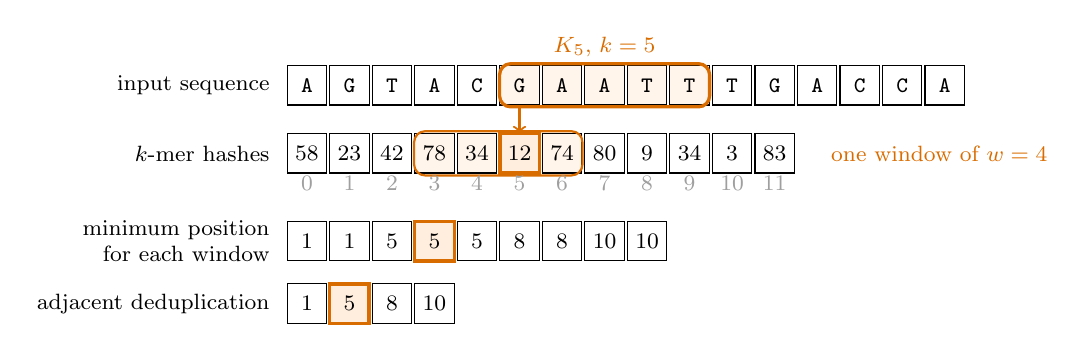
\begin{tikzpicture}[
  x=.54cm,
  y=.72cm,
  font=\footnotesize,
  cell/.style={draw,minimum width=.50cm,minimum height=.50cm,inner sep=0pt},
  tracked/.style={draw=orange!85!black,very thick,fill=orange!13,
                  minimum width=.50cm,minimum height=.50cm,inner sep=0pt},
  context/.style={draw,fill=orange!8,minimum width=.50cm,
                  minimum height=.50cm,inner sep=0pt}
]
  \node[anchor=east] at (4.35,4.10) {input sequence};
  \foreach \i/\v in {0/A,1/G,2/T,3/A,4/C,5/G,6/A,7/A,8/T,9/T,10/T,11/G,12/A,13/C,14/C,15/A}
    \node[cell] (s\i) at (5+\i,4.10) {\texttt{\v}};
  \foreach \i/\v in {5/G,6/A,7/A,8/T,9/T}
    \node[context] at (5+\i,4.10) {\texttt{\v}};
  \draw[orange!85!black,very thick,rounded corners]
    (9.53,3.72) rectangle (14.47,4.48);
  \node[orange!85!black] at (12,4.78) {$K_5$, $k=5$};

  \node[anchor=east] at (4.35,2.90) {$k$-mer hashes};
  \foreach \i/\v in {0/58,1/23,2/42,3/78,4/34,5/12,6/74,7/80,8/9,9/34,10/3,11/83}
    \node[cell] (h\i) at (5+\i,2.90) {\v};
  \foreach \i/\v in {3/78,4/34,6/74}
    \node[context] at (5+\i,2.90) {\v};
  \node[tracked] at (10,2.90) {12};
  \draw[orange!85!black,thick,rounded corners]
    (7.52,2.51) rectangle (11.48,3.29);
  \node[anchor=west,orange!85!black] at (17.10,2.90)
    {one window of $w=4$};
  \foreach \i in {0,...,11}
    \node[gray!75] at (5+\i,2.37) {\i};

  \node[anchor=east,align=right] at (4.35,1.35)
    {minimum position\\for each window};
  \foreach \i/\v in {0/1,1/1,2/5,3/5,4/5,5/8,6/8,7/10,8/10}
    \node[cell] at (5+\i,1.35) {\v};
  \node[tracked] at (8,1.35) {5};

  \node[anchor=east] at (4.35,.25) {adjacent deduplication};
  \foreach \i/\v in {0/1,1/5,2/8,3/10}
    \node[cell] at (5+\i,.25) {\v};
  \node[tracked] at (6,.25) {5};
  \draw[->,thick,orange!85!black] (s5.south) to[out=-90,in=90] (h5.north);
\end{tikzpicture}
\caption{Minimizer extraction for $k=5$ and $w=4$ with illustrative hashes.
Positions in this walkthrough are zero-based $k$-mer starts. BioSeqDB's packed
minimap-compatible record converts them to final-base positions. The
highlighted candidate has hash 12 and remains minimal for three consecutive
windows, so adjacent deduplication emits its position once.}
\label{fig:minimizer-walkthrough}
\end{figure}

Sketching and lookup are separate operations. The target side stores each seed
key together with an occurrence payload. At minimum, that payload identifies
the target sequence, position, and strand.

Figure~\ref{fig:seed-hash-table} uses fixed four-base seeds on both sides. The
symbols $h_1$, $h_2$, and $h_3$ are illustrative fingerprints rather than
outputs of a particular hash function.

\begin{figure}[htbp]
\centering
\begin{tikzpicture}[
  x=.88cm,
  y=.82cm,
  font=\footnotesize,
  >=Latex,
  stage/.style={draw,rounded corners,fill=blue!8,align=center,
                minimum height=.72cm},
  seq/.style={draw=orange!75!black,rounded corners,fill=orange!8,
              align=center,minimum height=.72cm},
  index/.style={draw,very thick,rounded corners,fill=yellow!14,
                align=left,inner sep=5pt},
  output/.style={draw=ForestGreen!70!black,rounded corners,
                 fill=green!7,align=left,inner sep=5pt}
]
  \node[font=\small\bfseries] at (3.1,4.55) {Build the reference index};
  \node[seq,minimum width=5.7cm] (ref) at (3.1,3.65)
    {reference: \texttt{GCTATTACCTTAATGTGATGGAC}};
  \node[stage,minimum width=5.7cm] (rseed) at (3.1,2.55)
    {extract $k=4$: \texttt{GCTA}@0, \texttt{TTAA}@9,
     \texttt{ATGT}@12};
  \node[stage,minimum width=5.7cm] (rhash) at (3.1,1.45)
    {hash: $h_1$, $h_2$, $h_3$};

  \node[index] (table) at (5.8,-1.10) {
    \begin{tabular}{@{}cl@{}}
      \textbf{key} & \textbf{occurrence payload} \\
      $h_1$ & $(\textit{ref},0,+)$ \\
      $h_2$ & $(\textit{ref},9,+)$ \\
      $h_3$ & $(\textit{ref},12,+)$
    \end{tabular}};

  \node[font=\small\bfseries] at (11.2,4.55) {Query the index};
  \node[seq,minimum width=5.2cm] (query) at (11.2,3.65)
    {query: \texttt{AGGCTATAACCCTAATGT}};
  \node[stage,minimum width=5.2cm] (qseed) at (11.2,2.55)
    {extract $k=4$: \texttt{GCTA}@2, \texttt{TAAC}@6,
     \texttt{ATGT}@14};
  \node[stage,minimum width=5.2cm] (qhash) at (11.2,1.45)
    {hash and look up: $h_1$, $h_4$, $h_3$};
  \node[output] (anchors) at (11.2,-1.10) {
    \begin{tabular}{@{}l@{}}
      candidate anchors\\
      $(q=2,t=0,+)$\\
      $(q=14,t=12,+)$
    \end{tabular}};

  \draw[->,thick] (ref) -- (rseed);
  \draw[->,thick] (rseed) -- (rhash);
  \draw[->,thick] (rhash) to[out=-90,in=160] (table.west);
  \draw[->,thick] (query) -- (qseed);
  \draw[->,thick] (qseed) -- (qhash);
  \draw[->,thick,blue!65!black] (qhash) to[out=-90,in=30] (table.east);
  \draw[->,thick,ForestGreen!70!black] (table.east) -- (anchors.west);
  \draw[->,thick,red!70!black] (qhash.east) to[out=0,in=90]
    node[pos=.55,right,align=left,text=red!70!black] {$h_4$: absent\\no anchor}
    (13.9,-.10);
\end{tikzpicture}
\caption{Reference-index construction and query lookup. Positions are seed
starts in this example. A usable seed index stores occurrence payloads rather
than hash values alone. A matching hash produces a candidate anchor. Seed
verification or downstream filtering is still required when the stored key
does not exclude collisions.}
\label{fig:seed-hash-table}
\end{figure}

Frequent seeds can produce very large occurrence lists. BioSeqDB can exclude
seeds whose target frequency exceeds a configured threshold before anchors
are constructed. This policy changes runtime and sensitivity, but not the
minimizer hashes. For a capped persistent index, the requested threshold must
not exceed the stored count cap.

\section{Methods for minimizer generation}









\section{TRASH}

%%%%% TRASH

Spaced seeds, linked seeds, and BLEND are comparative designs in this chapter.
The current BioSeqDB backends described later implement minimizer schemes.

The terms \emph{selection} and \emph{construction} describe different parts
of seeding. A minimizer selects one or more complete $k$-mers from a window by
hash rank. A spaced seed applies a binary mask to one fixed span and hashes
only retained positions. A linked seed, including a strobemer, chooses
components from separated downstream windows and combines them into one key.
The intervening sequence is not part of the linked key.

These choices respond differently to mutations. A substitution can change all
overlapping contiguous $k$-mers. A spaced mask ignores changes at omitted
positions. A strobemer can retain its component strings when mutations occur
between the selected windows. The linking rule must nevertheless be specified.
Without selection windows and a deterministic rule, concatenating arbitrary
$k$-mers does not define a reproducible strobemer. One possible rule selects
component $s_j$ by minimizing
$H(s_1\mathbin{\Vert}\cdots\mathbin{\Vert}s_{j-1}
\mathbin{\Vert}u)$ over candidates $u$ in the $j$th downstream window.

Figure~\ref{fig:seed-constructions} compares the three operations. The numeric
hash ranks are local examples. They do not imply that unrelated seed schemes
share a hash domain.

\begin{figure}[htbp]
\centering
\begin{tikzpicture}[
  x=.66cm,
  y=.64cm,
  font=\footnotesize,
  >=Latex,
  item/.style={draw=orange!75!black,rounded corners,fill=orange!8,
               align=center,minimum height=.72cm,inner xsep=5pt},
  op/.style={draw,rounded corners,fill=blue!8,align=center,
             minimum height=.72cm,inner xsep=5pt},
  chosen/.style={draw=ForestGreen!70!black,very thick,rounded corners,
                 fill=green!8,align=center,minimum height=.72cm,
                 inner xsep=5pt}
]
  \draw[rounded corners,gray!65] (.1,5.75) rectangle (20.3,8.45);
  \node[anchor=west,font=\small\bfseries] at (.45,8.12) {Minimizer};
  \node[item] (m1) at (2.7,7.35) {\texttt{GCTATTA}\\rank 161};
  \node[item] (m2) at (6.2,7.35) {\texttt{CTATTAC}\\rank 2};
  \node[item] (m3) at (9.7,7.35) {\texttt{TATTACC}\\rank 252};
  \node[item] (m4) at (13.2,7.35) {\texttt{ATTACCT}\\rank 69};
  \node[op] (mselect) at (9.7,6.10) {select lowest rank};
  \node[chosen] (mout) at (17.2,6.20) {minimum\\\texttt{CTATTAC}};
  \draw[->,thick] (m1.south) to[out=-90,in=170] (mselect.west);
  \draw[->,thick] (m2.south) to[out=-90,in=110] ($(mselect.north)+(-.35,0)$);
  \draw[->,thick] (m3.south) -- ($(mselect.north)+(.35,0)$);
  \draw[->,thick] (m4.south) to[out=-90,in=10] (mselect.east);
  \draw[->,thick] (mselect) -- (mout);

  \draw[rounded corners,gray!65] (.1,2.85) rectangle (20.3,5.50);
  \node[anchor=west,font=\small\bfseries] at (.45,5.18) {Spaced seed};
  \node[item] (sin) at (2.7,3.85)
    {\texttt{GCTATTA}\\\texttt{GATACTA}};
  \node[op] (mask) at (7.0,3.85) {mask \texttt{1011011}\\retain the 1 bits};
  \node[chosen] (skeep) at (11.5,3.85)
    {retained symbols\\\texttt{GTATA}\\\texttt{GTATA}};
  \node[op] (shash) at (16.0,3.85) {hash retained\\positions};
  \node[chosen] (sout) at (19.0,3.85) {same key};
  \draw[->,thick] (sin) -- (mask);
  \draw[->,thick] (mask) -- (skeep);
  \draw[->,thick] (skeep) -- (shash);
  \draw[->,thick] (shash) -- (sout);

  \draw[rounded corners,gray!65] (.1,-.65) rectangle (20.3,2.60);
  \node[anchor=west,font=\small\bfseries] at (.45,2.25) {Linked seed};
  \node[chosen] (st1) at (2.3,.55) {$s_1$\\\texttt{GCTA}};
  \node[op] (win2) at (6.0,.55)
    {$W_2(s_1)$\\\{\texttt{CCTT},\texttt{TTAA}\}};
  \node[chosen] (st2) at (9.2,.55) {choose\\\texttt{TTAA}};
  \node[op] (win3) at (12.6,.55)
    {$W_3(s_1,s_2)$\\\{\texttt{GTGA},\texttt{TGGA}\}};
  \node[chosen] (st3) at (15.9,.55) {choose\\\texttt{TGGA}};
  \node[item] (stout) at (19.0,.55)
    {\texttt{GCTA|}\\\texttt{TTAA|TGGA}};
  \draw[->,thick] (st1) -- (win2);
  \draw[->,thick] (win2) -- (st2);
  \draw[->,thick] (st2) -- (win3);
  \draw[->,thick] (win3) -- (st3);
  \draw[->,thick] (st3) -- (stout);
\end{tikzpicture}
\caption{Three seed constructions. A minimizer selects the lowest ranked
$k$-mer in a window. A spaced seed retains positions marked by a binary mask.
A linked seed chooses components from explicit downstream windows, where each
choice can depend on earlier components. The final linked key omits the bases
between the selected components.}
\label{fig:seed-constructions}
\end{figure}

\subsection{Fuzzy seed hashing with BLEND}

Conventional hashes are designed so a small input change produces an
unrelated output. That behavior is useful for uniform minimizer sampling, but
it prevents approximate seeds from meeting in a hash table. BLEND instead
uses a SimHash construction to make related seeds more likely to share a
fingerprint~\cite{blend}. BLEND-I tokenizes a contiguous seed into overlapping
substrings. BLEND-S applies the same principle to linked seed components.

Let a seed produce token hashes $g_1,\ldots,g_r$, each represented by $b$
bits. Bit $j$ of the fuzzy fingerprint can be written schematically as
\[
  f_j=\mathbf{1}\!\left[
      \sum_{q=1}^{r}\bigl(2g_{q,j}-1\bigr)>0
    \right].
\]
Thus each token contributes a positive or negative vote to every output bit.
With an odd token count, the displayed rule has no zero vote. A concrete
implementation also defines its behavior for even counts. Similar seeds share
many token hashes, so many votes remain unchanged. This raises the probability
of an equal fingerprint. It does not guarantee equality, and unrelated seeds
can still collide.

When BLEND supplies the rank for a minimizer, every candidate $k$-mer first
receives a fuzzy fingerprint and the window selects the lowest fingerprint.
Equal fingerprints must follow the minimizer implementation's stated tie
rule. For a linked seed, BLEND-S hashes the selected components and uses the
result directly as the lookup key.

Figure~\ref{fig:blend-fuzzy-hash} separates fingerprint construction from
index lookup. The bit strings are schematic. They illustrate voting rather
than a fixed BLEND parameter set.

\begin{figure}[htbp]
\centering
\begin{tikzpicture}[
  x=.64cm,
  y=.68cm,
  font=\footnotesize,
  >=Latex,
  seed/.style={draw=orange!75!black,rounded corners,fill=orange!8,
               align=center,minimum height=.78cm,inner xsep=3pt},
  blend/.style={draw=ForestGreen!70!black,rounded corners,fill=green!9,
                align=center,minimum height=.78cm,inner xsep=3pt},
  stage/.style={draw,rounded corners,fill=blue!8,align=center,
                minimum height=.78cm,inner xsep=3pt}
]
  \draw[rounded corners,gray!65] (.1,3.15) rectangle (20.5,6.80);
  \node[anchor=west,font=\small\bfseries] at (.45,6.45)
    {BLEND-I for a contiguous seed};
  \node[seed] (biin) at (2.1,5.45) {\texttt{GCTATTAC}};
  \node[seed] (biinb) at (2.1,4.25) {\texttt{GCTACTAC}};
  \node[stage] (tokens) at (6.1,4.85)
    {overlapping tokens\\\texttt{GCTA}, \texttt{CTAT}, \texttt{TATT}\\
     \texttt{ATTA}, \texttt{TTAC}};
  \node[stage] (bits) at (11.2,4.85)
    {ordinary token hashes\\as bit vectors};
  \node[blend] (vote) at (15.2,4.85)
    {signed vote\\in each bit};
  \node[blend] (bifp) at (18.5,4.85)
    {fuzzy\\fingerprint $f$};
  \draw[->,thick] (biin) -- (tokens);
  \draw[->,thick] (biinb) -- (tokens);
  \draw[->,thick] (tokens) -- (bits);
  \draw[->,thick] (bits) -- (vote);
  \draw[->,thick] (vote) -- (bifp);
  \node[align=center,text=black!70] at (10.0,3.65)
    {nearby seeds change some token votes and may share $f$};

  \draw[rounded corners,gray!65] (.1,-.55) rectangle (20.5,2.85);
  \node[anchor=west,font=\small\bfseries] at (.45,2.50)
    {BLEND-S and candidate lookup};
  \node[seed] (bsin) at (2.6,.85)
    {linked components\\\texttt{GCTA|TTAA|TGGA}};
  \node[stage] (bstok) at (7.1,.85)
    {component token\\hashes};
  \node[blend] (bsvote) at (10.8,.85)
    {bit vote\\fingerprint $f_s$};
  \node[stage] (lookup) at (14.0,.85)
    {index lookup\\by $f_s$};
  \node[stage] (cand) at (16.9,.85)
    {candidate\\occurrences};
  \node[blend] (verify) at (19.4,.85)
    {verify};
  \draw[->,thick] (bsin) -- (bstok);
  \draw[->,thick] (bstok) -- (bsvote);
  \draw[->,thick] (bsvote) -- (lookup);
  \draw[->,thick] (lookup) -- (cand);
  \draw[->,thick] (cand) -- (verify);
\end{tikzpicture}
\caption{Fuzzy hashing in BLEND. Token hashes vote independently on each
fingerprint bit. The upper panel shows a possible shared fingerprint for two
nearby seeds, not a guaranteed outcome. Index lookup therefore returns
candidates that still require verification or downstream filtering.}
\label{fig:blend-fuzzy-hash}
\end{figure}

\section{The minimap2 event contract}
\label{sec:minimap2-sketch}

Minimap2 uses two-bit nucleotide ranks
\[
  \eta(A)=0,
  \qquad
  \eta(C)=1,
  \qquad
  \eta(G)=2,
  \qquad
  \eta(T)=3.
\]
For a valid base code $c_i$, it updates forward and reverse-complement words
without rebuilding the $k$-mer
\[
\begin{aligned}
  F_i & = ((F_{i-1}\ll2)\mathbin{\vert}c_i)
          \mathbin{\&}(2^{2k}-1),\\
  R_i & = (R_{i-1}\gg2)\mathbin{\vert}
          ((3\mathbin{\oplus}c_i)\ll2(k-1)).
\end{aligned}
\]
The smaller word is canonical. A reversible integer mixing function maps it
to a well-distributed hash in the $2k$-bit domain. The candidate position is
the final base of the $k$-mer, and the strand bit records which orientation
provided the canonical word~\cite{minimap2_paper}.

The sliding minimum is maintained with a circular buffer of $w$ candidates
and one saved minimum. A new candidate replaces the saved minimum when its
hash is less than or equal to the current value. The less-than-or-equal rule
makes the entering candidate the rightmost equal minimum. When the saved
candidate expires, the ring is scanned from oldest to newest with the same
rightmost preference. The first complete window and the expiry branch also
report distinct identities tied with the selected hash. The final live
minimum is emitted when input ends.

These details make minimap2 output an event stream rather than one value for
each mathematical window. Algorithm~\ref{alg:minimap-scalar-events} gives the
essential state transitions. The event logic is shown separately from packed
record widths because the same semantics can be represented by different
integer layouts.

\begin{algorithm}[htbp]
\caption{Minimap-style scalar minimizer collection}
\label{alg:minimap-scalar-events}
\small
\textbf{Input:} sequence (S), (k), and window width (w)

\textbf{Output:} minimizer events in chronological order

\begin{enumerate}
  \item Initialize forward and reverse rolling words. Fill a circular buffer
        of (w) candidates with sentinels and set the current minimum to a
        sentinel.
  \item For each input symbol at position (i), construct one candidate.
    \begin{enumerate}
      \item If the symbol is ambiguous, reset both rolling words and the
            valid-run length. Use a sentinel candidate.
      \item Otherwise update (F) and (R). Once the valid run has length
            at least (k), hash the smaller word and attach position and
            strand. A palindromic word is represented according to the
            selected compatibility rule.
    \end{enumerate}
  \item Replace the next circular-buffer slot with the candidate.
  \item If the candidate hash is no greater than the current hash, emit the
        old live minimum when required and make the entering candidate the
        new minimum.
  \item Otherwise, if the overwritten slot held the current minimum, emit
        that event, rescan the ring, and retain the rightmost equal minimum.
        Emit other distinct identities tied in the required chronology.
  \item Handle the first complete window explicitly. After the final symbol,
        emit the last live minimum.
\end{enumerate}
\end{algorithm}

An ambiguous base and a storage-fragment boundary are not the same event. An
ambiguous base ends the run of valid $k$-mers. A storage boundary should be
invisible when the two fragments are adjacent parts of one logical sequence.
The collector must either continue its rolling and window state or replay
enough context to reconstruct the same state.

There is one deliberate difference between upstream minimap2 and BioSeqDB's
minimap-compatible scalar definition. Upstream minimap2 skips a palindromic
$k$-mer iteration because its strand is undefined. BioSeqDB advances the
window with a maximum-valued sentinel. The palindrome cannot become a
minimizer, but it consumes one chronological window slot. The CPU and GPU
implementations that claim the BioSeqDB minimap-compatible scheme follow this
sentinel rule.

\section{Data-independent sliding minima}
\label{sec:two-stack-minimum}

The scalar ring is efficient because a full rescan occurs only when the saved
minimum expires. Direct lane-wise vectorization changes the cost. If the
probability of one stream requesting a rescan is approximately $1/w$, then
$L$ independent vector lanes request at least one rescan with probability
\[
  1-\left(1-\frac{1}{w}\right)^L.
\]
For $w=10$ and four lanes this is about $34.4\%$. A vector implementation must
then mask unaffected lanes or move their state through a scalar slow path.
The vector instruction computes several hashes, but the control flow remains
irregular.

Three common sliding-minimum structures expose different tradeoffs.

\begin{table}[htbp]
\centering
\small
\begin{tabularx}{\linewidth}{p{.20\linewidth}XX}
\toprule
Method & Update rule & Consequence \\
\midrule
Circular buffer with rescan & Keep the current minimum and scan (w)
candidates when it expires & Small scalar state, but data-dependent work \\
Monotone deque & Remove expired values at the front and no-smaller entering
values at the back & Amortized linear work, but a data-dependent number of
pops per candidate \\
Block prefix and suffix minima & Precompute minima from each block boundary
and combine two values per window & Fixed work per block and regular lane-wise
execution \\
\bottomrule
\end{tabularx}
\caption{Alternative structures for a sliding-window minimum. The block
prefix and suffix form is useful for SIMD because each crossing window uses
one fixed comparison.}
\label{tab:sliding-minimum-formulations}
\end{table}

Partition the hash array into blocks of exactly $w$ values. For a position $i$
in block $B_q$, define
\[
  P_i=\min(a_{qw},\ldots,a_i),
  \qquad
  Q_i=\min(a_i,\ldots,a_{qw+w-1}).
\]
Here $P_i$ is a prefix minimum from the block start and $Q_i$ is a suffix
minimum to the block end. A window beginning at $j$ and ending at
$e=j+w-1$ satisfies
\[
  \min(a_j,\ldots,a_e)=\min(Q_j,P_e).
\]
A tie-aware implementation carries endpoint identities with each value. It can
therefore retain the leftmost and rightmost occurrences of an equal minimum
without rescanning the window.

\begin{figure}[htbp]
\centering
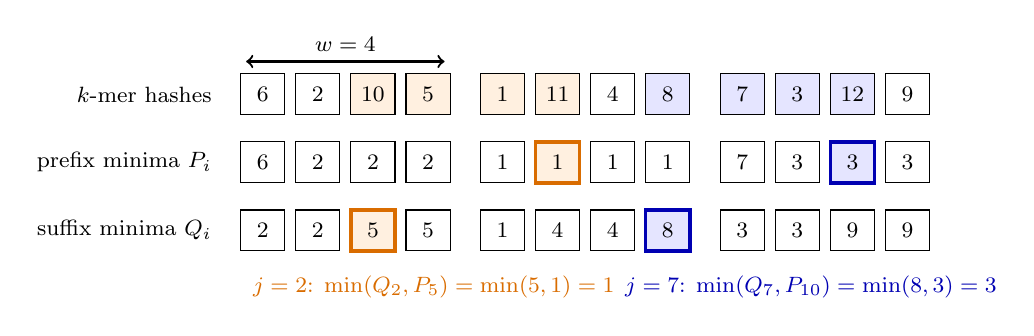
\begin{tikzpicture}[
  x=.70cm,
  y=.72cm,
  font=\footnotesize,
  cell/.style={draw,minimum width=.56cm,minimum height=.52cm,inner sep=0pt},
  first/.style={draw=orange!85!black,very thick,fill=orange!12,
                minimum width=.56cm,minimum height=.52cm,inner sep=0pt},
  second/.style={draw=blue!70!black,very thick,fill=blue!10,
                 minimum width=.56cm,minimum height=.52cm,inner sep=0pt}
]
  \node[anchor=east] at (4.25,3.25) {$k$-mer hashes};
  \foreach \i/\x/\v in {0/5.00/6,1/6.00/2,2/7.00/10,3/8.00/5,
                           4/9.35/1,5/10.35/11,6/11.35/4,7/12.35/8,
                           8/13.70/7,9/14.70/3,10/15.70/12,11/16.70/9}
    \node[cell] (a\i) at (\x,3.25) {\v};
  \foreach \i/\x/\v in {2/7.00/10,3/8.00/5,4/9.35/1,5/10.35/11}
    \node[cell,fill=orange!12] at (\x,3.25) {\v};
  \foreach \i/\x/\v in {7/12.35/8,8/13.70/7,9/14.70/3,10/15.70/12}
    \node[cell,fill=blue!10] at (\x,3.25) {\v};
  \draw[<->,thick] (4.70,3.83) -- (8.30,3.83)
    node[midway,above] {$w=4$};

  \node[anchor=east] at (4.25,2.05) {prefix minima $P_i$};
  \foreach \i/\x/\v in {0/5.00/6,1/6.00/2,2/7.00/2,3/8.00/2,
                           4/9.35/1,5/10.35/1,6/11.35/1,7/12.35/1,
                           8/13.70/7,9/14.70/3,10/15.70/3,11/16.70/3}
    \node[cell] (p\i) at (\x,2.05) {\v};
  \node[first] at (10.35,2.05) {1};
  \node[second] at (15.70,2.05) {3};

  \node[anchor=east] at (4.25,.85) {suffix minima $Q_i$};
  \foreach \i/\x/\v in {0/5.00/2,1/6.00/2,2/7.00/5,3/8.00/5,
                           4/9.35/1,5/10.35/4,6/11.35/4,7/12.35/8,
                           8/13.70/3,9/14.70/3,10/15.70/9,11/16.70/9}
    \node[cell] (q\i) at (\x,.85) {\v};
  \node[first] at (7.00,.85) {5};
  \node[second] at (12.35,.85) {8};

  \node[anchor=west,orange!85!black] at (4.65,-.15)
    {$j=2$: $\min(Q_2,P_5)=\min(5,1)=1$};
  \node[anchor=west,blue!70!black] at (11.40,-.15)
    {$j=7$: $\min(Q_7,P_{10})=\min(8,3)=3$};
\end{tikzpicture}
\caption{Sliding minima from blockwise prefixes and suffixes. Blocks have the
same width as the minimizer window. The two shaded crossing windows each use
one suffix value from the starting block and one prefix value from the ending
block.}
\label{fig:two-stack-minimum}
\end{figure}

\subsection{Rolling ntHash}
\label{sec:rolling-nthash}

SIMD-Minimizers combines blockwise minima with the ntHash family
\cite{nthash_2016,groot_koerkamp_simd_minimizers_2025}. Associate each base
with a pseudorandom word $f(b)$ and let $\operatorname{comp}(b)$ denote its
complementary base. For a rotation distance $r$, define
\[
\begin{aligned}
  H^F_i &= \bigoplus_{j=0}^{k-1}
    \operatorname{rotl}\!\left(f(s_{i+j}),r(k-1-j)\right),\\
  H^R_i &= \bigoplus_{j=0}^{k-1}
    \operatorname{rotl}\!\left(f(\operatorname{comp}(s_{i+j})),rj\right).
\end{aligned}
\]
After initialization, both states advance in constant time
\[
\begin{aligned}
  H^F_{i+1} &= \operatorname{rotl}(H^F_i,r)
    \mathbin{\oplus}\operatorname{rotl}(f(s_i),rk)
    \mathbin{\oplus}f(s_{i+k}),\\
  H^R_{i+1} &= \operatorname{rotr}(H^R_i,r)
    \mathbin{\oplus}\operatorname{rotr}
      (f(\operatorname{comp}(s_i)),r)
    \mathbin{\oplus}\operatorname{rotl}
      (f(\operatorname{comp}(s_{i+k})),r(k-1)).
\end{aligned}
\]
The canonical ntHash value used by SIMD-Minimizers is the wrapping sum of the
forward and reverse states. This hash family differs from minimap2's integer
mix of a canonical two-bit word. The selected minimizers can therefore differ
even when both implementations calculate their own algorithms correctly.

The published SIMD-Minimizers method divides the sequence into eight logical
chunks with enough overlap to cover every owned window. Corresponding
positions from the chunks occupy vector lanes. Rolling hashes and prefix or
suffix minima are updated in lock step. The algorithm uses a reduced hash key
for selection and resolves equal extremes through a canonical orientation of
the complete $(k+w-1)$-base window
\cite{groot_koerkamp_simd_minimizers_2025}. These choices define a seed
contract rather than a transparent optimization of minimap2.

\begin{table}[htbp]
\centering
\footnotesize
\setlength{\tabcolsep}{3.5pt}
\begin{tabularx}{\linewidth}{p{.16\linewidth}XXX}
\toprule
Property & Canonical minimizer abstraction & Minimap2 & SIMD-Minimizers \\
\midrule
Candidate key & Hash of one canonical $k$-mer & Integer mix of
$\min(F_i,R_i)$ & Rolling forward and reverse ntHash sum \\
Window minimum & Any lowest ranked candidate & Circular ring with expiry
rescans & Block prefix and suffix minima \\
Equal minima & Requires an explicit policy & Rightmost entering winner with
additional chronological tie events & Extreme endpoint selected from the
canonical orientation of the complete window \\
Parallel structure & Not specified & Sequential candidate stream & Eight
overlapped logical chunks processed lane-wise \\
Compatibility & Defined only after all policies are fixed & Minimap2 hash,
position, and event rules & Separate hash width, endpoint, and orientation
rules \\
\bottomrule
\end{tabularx}
\caption{The abstract minimizer definition does not determine an
interoperable seed stream. Minimap2 and SIMD-Minimizers complete the definition
in different ways.}
\label{tab:minimizer-algorithm-comparison}
\end{table}

\subsection{Chunked vector extraction}

A chunked extractor assigns each logical chunk an owned interval of candidate
positions. The chunk also reads a right context of at least $k+w-2$ bases when
ownership is defined by window starts. The first $k-1$ extra bases complete a
$k$-mer near the boundary. The remaining $w-1$ candidates complete windows
that begin in the owned interval. Equivalent left-context formulations are
possible, but ownership and context direction must agree.

Each vector lane advances through one logical chunk. The hash and sliding
minimum stages return chunk-local positions. Adding the chunk origin converts
them to absolute sequence positions. Collection then restores chunk order and
removes only repeated identities caused by neighboring windows or overlap.
Equal hashes at different positions remain distinct.

\begin{figure}[htbp]
\centering
\begin{tikzpicture}[
  x=.64cm,
  y=.68cm,
  font=\footnotesize,
  >=Latex,
  owned/.style={draw=blue!70!black,fill=blue!10,minimum height=.58cm},
  halo/.style={draw=orange!80!black,fill=orange!12,minimum height=.58cm},
  stage/.style={draw,rounded corners,fill=gray!8,align=center,
                minimum width=2.25cm,minimum height=1.05cm,inner sep=3pt}
]
  \node[anchor=east] at (1.30,6.05) {sequence $S$};
  \draw[thick] (1.55,5.72) rectangle (19.65,6.38);
  \foreach \x in {5.55,9.55,13.55,17.55}
    \draw[gray!70] (\x,5.72) -- (\x,6.38);
  \foreach \x/\v in {3.55/$C_0$,7.55/$C_1$,11.55/$C_2$,15.55/$C_3$}
    \node at (\x,6.05) {\v};
  \node at (18.60,6.05) {$\cdots$};

  \draw[owned] (1.55,4.55) rectangle (5.55,5.13);
  \draw[halo] (5.55,4.55) rectangle (7.55,5.13);
  \node at (3.55,4.84) {$C_0$ owned};
  \node at (6.55,4.84) {context};
  \draw[owned] (5.55,3.65) rectangle (9.55,4.23);
  \draw[halo] (9.55,3.65) rectangle (11.55,4.23);
  \node at (7.55,3.94) {$C_1$ owned};
  \node at (10.55,3.94) {context};
  \node[anchor=west] at (12.05,4.38)
    {$g=k+w-2$ bases of context};
  \node[anchor=west,gray!75] at (12.05,3.82)
    {remaining chunks follow the same rule};
  \draw[->] (3.55,5.70) -- (3.55,5.16);
  \draw[->] (7.55,5.70) -- (7.55,4.27);

  \node[stage] (lanes) at (2.15,1.55)
    {lane matrix\\$C_0[t]\quad C_1[t]$\\$C_2[t]\quad C_3[t]$};
  \node[stage] (hash) at (6.25,1.55)
    {rolling hashes\\$h_{0,t}\quad h_{1,t}$\\$h_{2,t}\quad h_{3,t}$};
  \node[stage] (minimum) at (10.35,1.55)
    {window argmin\\$p_{0,t}\quad p_{1,t}$\\$p_{2,t}\quad p_{3,t}$};
  \node[stage] (absolute) at (14.45,1.55)
    {absolute positions\\$p_{c,t}+o_c$};
  \node[stage] (collect) at (18.55,1.55)
    {collected output\\$p_0,p_1,p_2,\ldots$\\deduplicate identity};
  \draw[->,thick] (lanes) -- (hash);
  \draw[->,thick] (hash) -- (minimum);
  \draw[->,thick] (minimum) -- (absolute);
  \draw[->,thick] (absolute) -- (collect);
  \draw[->,thick] (7.55,3.55) to[out=-90,in=90] (lanes.north);
\end{tikzpicture}
\caption{Vectorized minimizer extraction over logical chunks. Each chunk owns
a disjoint range and reads enough context to complete its boundary windows.
Lane-wise rolling hashes and minima produce local positions. Adding each chunk
origin and deduplicating full identities yields a global sketch. The symbolic
chunk size is an execution parameter rather than part of minimizer semantics.}
\label{fig:vector-minimizer-pipeline}
\end{figure}

Lane-wise output is naturally ordered by vector step rather than by logical
chunk. A transpose converts vectors of simultaneous events into one sorted
list per chunk. Adjacent deduplication is valid within each list because its
positions are ordered. The last emitted position for each chunk is an
independent carry value. It must not be mistaken for one value shared across
all rows.

\begin{figure}[htbp]
\centering
\begin{tikzpicture}[
  x=.62cm,
  y=.62cm,
  font=\footnotesize,
  >=Latex,
  cell/.style={draw,minimum width=.52cm,minimum height=.52cm,inner sep=0pt},
  trace/.style={draw=orange!85!black,very thick,fill=orange!12,
                minimum width=.52cm,minimum height=.52cm,inner sep=0pt},
  carry/.style={draw=gray!70,fill=gray!10,text=gray!80,
                minimum width=.52cm,minimum height=.52cm,inner sep=0pt}
]
  \node[font=\small\bfseries] at (2.50,4.15) {events by vector step};
  \foreach \r/\c/\v in {0/0/1,0/1/12,0/2/23,0/3/30,
                           1/0/1,1/1/13,1/2/23,1/3/35,
                           2/0/2,2/1/13,2/2/23,2/3/35,
                           3/0/4,3/1/13,3/2/23,3/3/36}
    \node[cell] at (1+\c,3-\r) {\v};
  \foreach \r/\v in {0/1,1/1,2/2,3/4}
    \node[trace] at (1,3-\r) {\v};

  \node[font=\small\bfseries] at (9.00,4.15) {one sorted row per chunk};
  \foreach \r/\c/\v in {0/0/1,0/1/1,0/2/2,0/3/4,
                           1/0/12,1/1/13,1/2/13,1/3/13,
                           2/0/23,2/1/23,2/2/23,2/3/23,
                           3/0/30,3/1/35,3/2/35,3/3/36}
    \node[cell] at (7.5+\c,3-\r) {\v};
  \foreach \c/\v in {0/1,1/1,2/2,3/4}
    \node[trace] at (7.5+\c,3) {\v};

  \draw[->,very thick] (5.05,1.5) -- (6.75,1.5)
    node[midway,above] {transpose};
  \draw[->,very thick] (11.65,1.5) -- (13.15,1.5)
    node[midway,above,align=center] {deduplicate\\and append};

  \node[font=\small\bfseries] at (16.1,4.15) {ragged chunk outputs};
  \node at (14.2,3.65) {$\operatorname{last}[c]$};
  \foreach \r/\v in {0/0,1/11,2/23,3/30}
    \node[carry] at (14.2,3-\r) {\v};
  \foreach \x/\v in {15.5/1,16.5/2,17.5/4}
    \node[trace] at (\x,3) {\v};
  \foreach \x/\v in {15.5/12,16.5/13}
    \node[cell] at (\x,2) {\v};
  \node[anchor=west,gray!75] at (15.25,1) {no new position};
  \foreach \x/\v in {15.5/35,16.5/36}
    \node[cell] at (\x,0) {\v};
  \foreach \r in {0,...,3}
    \draw[->,gray!70] (14.55,3-\r) -- (15.10,3-\r);
\end{tikzpicture}
\caption{Transposition and boundary deduplication for four logical chunks.
The input rows are vector steps and the columns are chunks. Transposition
makes each chunk a sorted row. Each row has its own previous-position carry,
shown in gray. Only new positions are appended, so padding cells are not part
of the output.}
\label{fig:transpose-dedup}
\end{figure}

\section{BioSeqDB minimizer backends}

BioSeqDB separates a \emph{seed scheme} from an \emph{execution backend}. The
scheme determines the candidate hash, tie policy, ambiguity behavior, position
encoding, and fragment semantics. The backend determines where and how those
rules are executed. The ExactSimd label covers two distinct selection routes.
Its continuation route uses the Scalar candidate order, while its resident
vector-stream route has a different ordering contract. PaperNtHashSimd defines
another incompatible scheme.

Persistent-index metadata records the seed-scheme identity and the producing
backend identity and revision. Query preparation must match these values.
Rebuilding only the query sketch cannot repair a mismatch.

\subsection{Scalar reference}

Scalar is the portable implementation of BioSeqDB's minimap-compatible event
contract. It uses the two-bit canonical word, the minimap-style integer mix,
rightmost equal-minimum selection, chronological tie events, sentinel
palindromes, ambiguity resets, and a final flush. It is also the default CPU
selection when no more specific backend is requested.

The scalar algorithm is important even when a faster backend is available. It
states the complete event order without lane transposition or tile ownership.
The ExactSimd continuation route targets the same output. VulkanSegment targets
the same DNA4 output on a device. The resident ExactSimd route and
PaperNtHashSimd have separate contracts.

\subsection{ExactSimd continuation}
\label{sec:exact-simd}

The ExactSimd continuation route uses vector operations to reproduce the
BioSeqDB stream that is compatible with minimap across a fragmented sequence. A fragment
boundary does not reset biological state. The continuation retains at most the
following bounded information:

\begin{itemize}
  \item the final $k-1$ normalized symbols needed by the rolling $k$-mer
  \item fewer than one pending vector group and its absolute positions
  \item the last $w-1$ candidates needed to complete crossing windows
  \item the current minimum and the chronology needed for event emission
\end{itemize}

The bound depends on $k$, $w$, and vector width, not on the total sequence
length or number of fragments. When the next fragment arrives, it completes
the pending group and continues the same logical stream. An ambiguous symbol
instead clears the rolling $k$-mer context and inserts the scheme's sentinel
candidate into the existing window chronology.

The common $k=15,w=10$ specialization processes eight consecutive candidate
positions per block. It needs $k+8-1=22$ base codes to form those overlapping
$k$-mers. The codes are packed into a machine word, and fixed shifts extract
the eight forward words. Reverse-complement words are constructed in a second
vector stream. The lower word in each orientation pair is mixed with the
minimap hash, while position and strand remain attached as separate metadata.

After minimap-style scrambling, window reduction uses the minimap-compatible
less-than-or-equal rule.
This is more work than selecting only one prefix and one suffix value, but it
preserves the required rightmost winner and the event order around expiry.
Ordinary windows emit through a compact vector path. Equal-hash candidates at
different positions enter a separate tie-aware path that reconstructs all
required chronological events. The split is an execution choice and does not
change observable results.

\begin{algorithm}[htbp]
\caption{ExactSimd block with bounded continuation}
\label{alg:exact-b8}
\small
\textbf{Input:} the continuation state and the next vector group of bases

\textbf{Output:} chronological minimap-compatible events and updated state

\begin{enumerate}
  \item Join saved $k$-mer context with the new symbols and construct the
        overlapping forward and reverse-complement words.
  \item Select the canonical word in each lane. Replace palindromes and
        candidates crossing ambiguity with maximum-valued sentinels.
  \item Apply the minimap integer hash and attach absolute position, strand,
        and chronological identity.
  \item Join the saved $w-1$ candidate tail with the new candidates. Reduce
        each complete window with the rightmost equal-minimum rule.
  \item Derive entering-minimum, expiry, first-window, and final-event masks.
  \item Compact ordinary events directly. For an actual equal-hash,
        different-identity tie, recover and compact the required events in
        chronological order.
  \item Save the final $k-1$ symbols, $w-1$ candidates, pending symbols, and
        current minimum for the next fragment.
\end{enumerate}
\end{algorithm}

ExactSimd is selected explicitly. If its checked path cannot adapt or
materialize an admitted input shape, an unsupported representation or
position range is reported as an error. The request does not fall back to
Scalar and is not reinterpreted by a different seed scheme.

\subsection{PNT1 as a separate ntHash scheme}
\label{sec:pnt1}

PNT1 applies the data-independent SIMD-Minimizers structure but defines a
BioSeqDB-specific persistent scheme.
Its candidate key is the full wrapping 32-bit sum
\[
  h_i=H^F_i+H^R_i\pmod{2^{32}},
\]
and its $k$-mer strand records whether $H^R_i<H^F_i$. It does not use
minimap2's two-bit canonical word or integer mix.

PNT1 also differs from the published SIMD-Minimizers endpoint rule. The
published algorithm chooses one equal extreme from the orientation of the
complete window. PNT1 retains the leftmost and rightmost identities attaining
the minimum. It emits the left identity first, followed by a distinct right
identity, then removes identical adjacent events. This rule is deterministic
for event identity and remains symmetric with respect to the two extremes. It
does not reproduce minimap2 chronology.

Eight logical streams are retained independently of the physical vector
width. A target with four 32-bit lanes uses two vector registers per step. A
target with eight lanes uses one. Logical stream count is therefore part of
the algorithm, while register count is a dispatch property. The streams
overlap enough to complete boundary windows. Bounded first- and last-event
state suppresses duplicate records at the seven stream joins.

Persisting a PNT1 index over fragmented storage uses bounded replay. For an
owned core interval $[c_\ell,c_h)$, the producer reads a halo on each side,
runs the PNT1 collector, translates local positions to global positions, and
retains only positions in the half-open core. Neighboring cores have disjoint
ownership, so one event cannot be published twice. Sorting by hash and encoded
position establishes a canonical persistent order even though append order
across lock-step logical streams is not an API guarantee.

PNT1 currently specializes the common $k=15,w=10$ DNA4 case and requires a
32-bit hash field. These constraints are visible at admission. A PNT1 index is
never queried through the Scalar or ExactSimd scheme merely because all three
outputs are called minimizers.

\subsection{Vulkan tile extraction}
\label{sec:vulkan-minimizers}

VulkanSegment applies the BioSeqDB minimap-compatible hash and event state
machine to packed sequences on a compute device. The main benefit is not an
alternative seed definition. It is the ability to keep packed bases,
minimizers, seed hits, and later mapping stages on the same device. Avoiding a
host round trip can matter more than an isolated hash-loop improvement.

Candidate positions within one tile are processed in sequence because the
rolling word and window minimum depend on prior candidates. Parallelism comes
from many tiles scheduled across device invocations. Each tile starts before
its owned trigger interval and replays enough context to reconstruct the
rolling and window state. It emits only events whose trigger position lies in
its half-open owned interval. Replay can overlap, but ownership does not.

Output cardinality is data dependent because ties and expiry can produce more
than one event. The compact route therefore uses three stages:

\begin{enumerate}
  \item Run the state machine in count mode to obtain the number of admitted
        events for every tile.
  \item Apply an exclusive prefix scan to the tile counts and allocate one
        exact output interval for each tile.
  \item Replay the same state machine in emit mode and write each event to its
        assigned interval.
\end{enumerate}

This process gives deterministic allocation and tile order without reserving
one output record per input base. A persistence-oriented route can instead
append to a proved capacity and establish order with a stable device sort.

For DNA4, VulkanSegment is intended to reproduce the scalar BioSeqDB event
stream exactly. The current DNA5 and generic packed routes have a weaker
contract. They retain every scalar event but may add a bounded number of
events near tile boundaries and invalid-symbol transitions. This distinction
affects downstream workload and is therefore part of backend selection. It is
not described as exact minimap compatibility.

\subsection{Comparison and selection}
\label{sec:minimizer-selection}

Table~\ref{tab:bioseqdb-minimizer-backends} summarizes the four choices. A
stored index fixes the seed scheme, producer identity, and revision before
backend admission is evaluated.

\begin{table}[htbp]
\centering
\footnotesize
\setlength{\tabcolsep}{3.5pt}
\begin{tabularx}{\linewidth}{p{.16\linewidth}p{.21\linewidth}XX}
\toprule
Backend & Seed contract & Main execution method & Principal constraints \\
\midrule
Scalar & BioSeqDB minimap-compatible & Rolling two-bit words and circular
window buffer & Portable default, sequential candidate stream \\
ExactSimd continuation & Same as Scalar & Vector candidate construction with
bounded fragment continuation and exact tie recovery & Indexed and fragmented
route, with the main specialization at $k=15,w=10$ \\
ExactSimd resident & Resident vector-stream contract & Full-resident vector
streams rank candidates before minimap scrambling & Transient no-index use
only when both full-resident sides use this route \\
PNT1 & Versioned PNT1 contract & Eight logical ntHash streams with
block minima and bounded stream-boundary deduplication & Packed DNA4,
$k=15,w=10$, full 32-bit hash, compatible PNT1 index \\
VulkanSegment & BioSeqDB minimap-compatible for DNA4 & Device tiles with
context replay, half-open ownership, and count or emit passes & Device and
buffer admission, exact DNA4 behavior, bounded conservative DNA5 behavior \\
\bottomrule
\end{tabularx}
\caption{BioSeqDB minimizer backends. Scalar and the ExactSimd continuation
route share one seed scheme. The resident ExactSimd route is distinct. PNT1 is
a different persistent scheme. VulkanSegment shares the
minimap-compatible candidate definition but currently has a
representation-dependent boundary contract.}
\label{tab:bioseqdb-minimizer-backends}
\end{table}

The practical selection rules follow directly:

\begin{enumerate}
  \item Require the query to match the target index's seed scheme, producer
        identity and revision, and hash, tie, position, and ambiguity contract.
  \item For the minimap-compatible CPU scheme, use Scalar by default. Indexed
        ExactSimd work requires the continuation route. The resident route is
        valid only when one transient operation owns two compatible resident
        inputs.
  \item Use PNT1 only with an index produced by PNT1. Treat changing to PNT1
        as an index migration.
  \item Use VulkanSegment when the device route is admitted and subsequent
        stages can consume its resident output. Apply the documented DNA4 or
        DNA5 semantic contract rather than treating both as identical.
  \item Reject a failure after a specific vector or device backend has been
        selected. Runtime substitution must not hide a scheme or semantic
        change.
\end{enumerate}

\subsection{Limitations}
\label{sec:minimizer-limitations}

The current backends do not form one uniform performance ladder. ExactSimd's
two selection routes are not lookup-compatible even though they share one
backend label. Its most regular continuation specialization is limited to the
common $k=15,w=10$ shape.
PNT1 has the same parameter restriction and additionally requires packed
DNA4, the complete 32-bit hash, and a supported vector width. VulkanSegment
obtains parallelism across tiles rather than across dependent positions within
one tile. Its compact output route repeats computation in count and emit mode.

The remaining representation difference is also significant. DNA4 has an
exact device contract. DNA5 currently has a conservative superset contract,
which can increase lookup and chaining work even when no scalar seed is lost.
Applications requiring identical event streams across all representations
must select an exact CPU backend until the device contract is strengthened.

No seed scheme avoids the sensitivity and frequency tradeoff. Increasing $w$
reduces sketch density and index cost, but raises the length of a conserved
region needed to retain a shared minimizer. A larger $k$ reduces random and
repetitive hits, but makes seeds less tolerant of substitutions and small
indels. Fuzzy hashes and linked seeds offer different tradeoffs, but introduce
their own collision, verification, and parameter requirements. These choices
should be evaluated as complete seed and index configurations rather than as
isolated hash functions.

\section{Conclusion}

Minimizer extraction consists of three distinct decisions. The seed scheme
defines candidate hashes and event semantics. The execution algorithm
maintains sliding minima and fragment state. The index maps selected keys to
target occurrences. Correct query processing requires all three decisions to
agree with the stored target index.

Minimap2 uses canonical two-bit $k$-mers, an integer mixing function, and a
rightmost chronological event rule. SIMD-Minimizers replaces rescans with
rolling ntHash and blockwise prefix or suffix minima, while also defining a
different endpoint and orientation policy. BioSeqDB preserves the minimap
scheme in Scalar and the ExactSimd continuation route, retains a separate
resident ExactSimd route for transient resident inputs, provides PNT1 as a
versioned ntHash scheme, and executes minimap-style extraction on Vulkan tiles when the input
representation is admitted. Persisted scheme, producer, and revision fields
prevent an optimization from silently changing the seed set consumed by
lookup and chaining.

%% TRASH

\section{Why minimizers, and why does this chapter exist?}
\label{sec:why-minimizers}

Chapter~\ref{r:{biology}} introduced the seed--chain--extend
pipeline used by every modern aligner.  In that pipeline, the
\emph{minimizer collector} is the only stage whose runtime cost is
strictly linear in the input length and not bounded by the alignment
depth: it must visit every base of every sequence it processes,
turning each $k$-mer into a hash, and selecting the
window-minimum of every $w$ consecutive $k$-mers as the
\emph{minimizer} for that window.

For our user-stated benchmarking goal -- pairs of ${\sim}10^6$ bp
sequences aligned against ${\sim}10^7$ bp references at PacBio HiFi
error rates -- the minimizer step accounts for roughly 8\,\% of the
total wall-clock per pair on the scalar pipeline, and up to 25\,\%
when a naive SIMD port has been written. That is the gap this
chapter is about.  Concretely:

\begin{itemize}
\item \textbf{Goal 1} (already met before this chapter starts).
  bioseq's \emph{scalar} pipeline must be within $\pm 10\,\%$ of
  minimap2's wall-clock on the long-sequence regime.  Met by the
  per-seed-pair gap-fill rewrite documented in V3 of the engineering
  report~\cite{bioseq_eng_report_v1}.
\item \textbf{Goal 2} (the topic of this chapter).
  bioseq's \emph{SIMD} pipeline must be at least 10\,\% faster than
  the scalar pipeline.  After a year of incremental work we sit
  marginally outside the goal on every length bucket: $-8.4\,\%$ at
  52\,kbp, $-8.8\,\%$ at 903\,kbp, $-4.9\,\%$ at 5\,Mbp (means of three
  runs).  The variance across runs occasionally clears the bar (V12
  individual runs at $-9.7\,\%$ to $-12\,\%$ have been seen on a
  quiescent host), but the mean reported here is the load-bearing
  number.  This chapter explains why every percentage point was so
  hard-won.
\end{itemize}

Figure~\ref{fig:headline-result} states the bottom line: across our
five sequence-length buckets, the V13 collector
(\texttt{collect\_minimizers\_two\_stack\_nthash\_v3}, the
production minimizer at the time of writing) is the fastest of the
SIMD configurations, and at every length except the 5\,Mbp XL bucket
it is also faster than the scalar baseline by 5--9\,\%.

% \begin{figure}[ht]
%   \centering
%   \begin{CacheMeCode}{python, custom include command={\input{\robExtAddCachePathAndName{\robExtFinalHash.pgf}}}, set placeholder eval={__LINEWIDTH__}{\lenToCmNoUnit[in]{\linewidth}}}
%     import matplotlib.pyplot as plt
%     import matplotlib
%     import numpy as np
%     matplotlib.use("pgf")
%     matplotlib.rcParams.update({
%       "font.family": "serif",
%       "font.serif": [],
%       "text.usetex": True,
%     })
%     fig, ax = plt.subplots()
%     fig.set_size_inches(__LINEWIDTH__, 0.55*__LINEWIDTH__, forward=True)
%     buckets = ['47 kbp', '49 kbp', '52 kbp', '903 kbp', '5.0 Mbp']
%     scalar = [14.56, 14.94, 15.09, 188.93, 1171.0]
%     simd_v6 = [15.21, 15.90, 16.05, 201.68, 1207.99]
%     v8_two_stack = [14.64, 15.07, 15.24, 183.77, 1131.87]
%     v12_v13 = [13.78, 14.02, 13.82, 172.38, 1113.3]
%     minimap2 = [20.11, 20.10, 20.13, 190.95, 1060.13]
%     x = np.arange(len(buckets))
%     width = 0.16
%     ax.bar(x - 2*width, minimap2, width, label='minimap2',
%            color='#000000')
%     ax.bar(x - width,   scalar,    width, label='scalar (baseline)',
%            color='#909090')
%     ax.bar(x,           simd_v6,   width, label='V6 SIMD (rescan)',
%            color='#1f77b4')
%     ax.bar(x + width,   v8_two_stack, width, label='V8 two-stack',
%            color='#2ca02c')
%     ax.bar(x + 2*width, v12_v13,   width, label='V13 (production)',
%            color='#d62728')
%     ax.set_xticks(x)
%     ax.set_xticklabels(buckets)
%     ax.set_yscale('log')
%     ax.set_ylabel('Wall-clock per pair (ms, log scale)', fontsize=8)
%     ax.set_title('End-to-end pipeline wall-clock per length bucket', fontsize=9)
%     ax.tick_params(axis='both', labelsize=7)
%     ax.legend(fontsize=7, frameon=False, loc='upper left', ncol=2)
%     ax.grid(True, alpha=0.3, axis='y', which='both')
%     print(get_filename_from_extension(".pgf"))
%     plt.savefig(get_filename_from_extension(".pgf"), bbox_inches="tight")
%   \end{CacheMeCode}
%   \caption{End-to-end pipeline wall-clock per pair, length bucket on
%     the X axis (log Y). \textsc{Scalar} is the baseline, \textsc{V6}
%     is the naive SIMDification of minimap2's rescan loop,
%     \textsc{V8} is the two-stack port from the SIMD-Minimizers paper
%     of Groot Koerkamp \&
%     Martayan~\cite{groot_koerkamp_simd_minimizers_2025}, and
%     \textsc{V13} is the production state after dual-stream
%     interleaving, forced inlining, and the
%     \texttt{mm\_est\_err} sort-free prefix-count rewrite.  The
%     minimap2 reference is included for orientation. On every bucket
%     except XL, V13 is the fastest of all five rows.}
%   \label{fig:headline-result}
% \end{figure}

\section{What a minimizer collector actually does}
\label{sec:what-is-minimizer}

Before we dive into the SIMD work, it pays to spend a page or two on
what the data looks like and how the original scalar algorithm gets
the answer.  This section is aimed at a reader who has seen the
phrase ``minimizer'' in passing -- e.g.\ from a Kraken or a minimap2
paper -- but has never written or read minimizer code.

Conceptually, a minimizer collector is a function
\[
\mathrm{collect\_minimizers}\colon \Sigma^* \times \mathbb{N} \times \mathbb{N}
\;\to\; \mathcal{P}\!\big(\;(\text{hash},\,\text{position},\,\text{strand})\;\big)
\]
that takes a sequence over the four-letter DNA alphabet, plus
parameters $w$ (window size) and $k$ ($k$-mer length), and returns a
set of triples that uniquely identify selected $k$-mers in the input.
The triples are what downstream stages -- chaining, error estimation,
seed-hit collection -- consume.

\begin{figure}[ht]
  \centering
  \begin{tikzpicture}[x=0.4cm, y=0.4cm, >=Latex]
    \foreach \i/\letter in {0/A,1/C,2/T,3/G,4/T,5/A,6/G,7/T,8/A,9/C,10/G,11/T,12/T,13/A}
        \node[minimum width=0.4cm,inner sep=0pt,font=\ttfamily\small] at (\i,0) {\letter};

    \foreach \i/\hashval in {0/13,1/20,2/27,3/34,4/41}
    {
      \pgfmathsetmacro{\xs}{\i - 0.2}
      \pgfmathsetmacro{\xe}{\i + 3.8}
      \pgfmathsetmacro{\yp}{-1.0 - \i*0.8}
      \draw[rounded corners=1pt, color=blue!50!gray, thick]
        (\xs, \yp) rectangle (\xe, \yp+0.6);
      \node[font=\tiny, color=blue!50!gray, anchor=west] at (\xe + 0.1, \yp+0.3)
        {kmer$_\i$ (h=\hashval)};
    }
    \node[font=\tiny, anchor=west, color=blue!50!gray]
      at (0, -5.6) {(kmers $k=4$ shown for first 5 positions)};

    \draw[rounded corners=1pt, color=ForestGreen, thick]
      (-0.3, -7.0) rectangle (8.3, -6.4);
    \node[font=\scriptsize, color=ForestGreen, anchor=west]
      at (-0.3, -7.6) {window of $w=4$ consecutive $k$-mers ($w+k-1=7$ bases wide)};
  \end{tikzpicture}
  \caption{The data the collector operates on. A sequence of 14
    bases produces overlapping $k=4$-mers
    (kmer$_0$, kmer$_1$, \ldots). The collector slides a
    window of $w=4$ consecutive $k$-mers (so $w+k-1=7$ bases wide)
    across the sequence and emits, for each window, the position of
    the $k$-mer with the smallest hash. A naive output would have
    one entry per window; a smart implementation deduplicates
    adjacent windows that share the same minimizer position.}
  \label{fig:minimizer-data}
\end{figure}

The intuition for \emph{why} a minimizer is a useful seed is in the
seed-stage discussion of Chapter~\ref{r:{biology}}:
the same $k$-mer is selected as the minimizer of every
overlapping window that contains it as the smallest hash, so two
sequences that share a contiguous identical region are very likely
to share at least one minimizer position there. The seed
collection then becomes a hash-table intersection rather than a
substring search, which is the entire reason any of this is fast.

\subsection{The minimap2 hash}
\label{sec:hash64}

Random minimizers depend critically on the hash function used to
order $k$-mers.  Three properties matter:

\begin{enumerate}
\item \textbf{Avalanche.} A single bit flip in the $k$-mer should
  change roughly half the bits of the hash output -- otherwise
  GC-rich and AT-rich windows occupy different
  hash-value subspaces and the minimizer set becomes biased.
\item \textbf{Reversibility.} The hash should be a
  bijection on its $\mathrm{2k}$-bit input domain, so that no two
  $k$-mers collide.  This is implementable with a sequence of
  reversible mixing operations
  (XOR, addition, multiplication by an odd constant, shifts).
\item \textbf{Cheap to evaluate.} The minimizer collector evaluates
  the hash once per $k$-mer position, so on a 1\,Mbp pair it runs
  the hash $2 \cdot 10^6$ times. Each cycle counts.
\end{enumerate}

minimap2 uses a hand-tuned 64-bit integer mix attributed to Thomas
Wang~\cite{wang_inthash}, applied to the bit-packed
$2k$-bit forward $k$-mer encoding (or to the reverse-complement
$k$-mer, whichever is lexicographically smaller -- this is the
\emph{canonical-strand} optimisation):

\begin{verbatim}
static inline uint64_t hash64(uint64_t key, uint64_t mask) {
    key = (~key + (key << 21)) & mask;        // key = key * 2097151 - 1
    key = key ^ (key >> 24);
    key = ((key + (key << 3)) + (key << 8)) & mask;   // * 265
    key = key ^ (key >> 14);
    key = ((key + (key << 2)) + (key << 4)) & mask;   // * 21
    key = key ^ (key >> 28);
    key = (key + (key << 31)) & mask;
    return key;
}
\end{verbatim}

Each pass alternates a multiplication-by-odd-constant (implemented as
a few \texttt{shift\,+\,add} pairs to be portable to
HP\,9000-class hardware where multiplication was slow in 1997) with
an XOR with a shifted version of itself.  The composite is
reversible (each stage is reversible) and has good
avalanche~\cite{wang_inthash}, but the dependency chain is
\textbf{seven stages deep}.  When the loop is in scalar code, the
out-of-order engine schedules these against the rest of the body and
hides the latency.  In the SIMD path the seven stages become a
seven-deep fused dependency chain on a single SIMD register, and they
end up dominating the inner loop -- a fact that drives most of the
optimisation work later in the chapter
(see~\S\ref{sec:v8-defer-scramble} for the eventual fix).

\subsection{The original minimap2 algorithm}

\texttt{mm\_sketch} in
\path{bench/tool_minimap2/minimap2/sketch.c} is the canonical scalar
minimizer collector.  Algorithm~\ref{alg:mm-sketch} captures the hot
path; for clarity we have stripped the homopolymer compression
branch and the bookkeeping for tied hashes.

\begin{algorithm}[H]
\caption{\texttt{mm\_sketch} (simplified; minimap2 \texttt{sketch.c})}
\label{alg:mm-sketch}
\small
\begin{algorithmic}[1]
\Require sequence $s$, window size $w$, $k$-mer length $k$
\State $\textit{buf}[0..w-1] \gets \infty$ \Comment{circular buffer of recent $k$-mer info}
\State $\textit{min} \gets \infty$, $\textit{min\_pos} \gets -1$
\State $\textit{kmer}[0] \gets 0$, $\textit{kmer}[1] \gets 0$ \Comment{forward / RC}
\State $\textit{shift1} \gets 2(k-1)$
\For{$i \gets 0$ to $|s|-1$}
    \State $c \gets \textit{seq\_nt4\_table}[s[i]]$ \Comment{ACGT $\to$ 0..3}
    \State $\textit{kmer}[0] \gets ((\textit{kmer}[0] \ll 2)\;|\;c)\,\&\,\textit{mask}$ \Comment{forward}
    \State $\textit{kmer}[1] \gets (\textit{kmer}[1] \gg 2)\;|\;((3 \oplus c) \ll \textit{shift1})$ \Comment{RC}
    \If{$\textit{kmer}[0] = \textit{kmer}[1]$} \Comment{palindrome}
        \State \textbf{continue} \Comment{strand undefined; skip}
    \EndIf
    \State $z \gets \textit{kmer}[0] < \textit{kmer}[1] \;?\; 0 : 1$ \Comment{strand}
    \State $\textit{info}.x \gets \textit{hash64}(\textit{kmer}[z]) \ll 8 \;|\; \textit{kmer\_span}$
    \State $\textit{info}.y \gets (i \ll 1)\;|\;z$
    \State $\textit{buf}[\textit{buf\_pos}] \gets \textit{info}$
    \If{$\textit{info}.x \le \textit{min}.x$}                                  \Comment{new minimum}
      \State \textbf{emit} $\textit{min}$ if armed
      \State $\textit{min} \gets \textit{info}$, $\textit{min\_pos} \gets \textit{buf\_pos}$
    \ElsIf{$\textit{buf\_pos} = \textit{min\_pos}$}                          \Comment{old min slid out}
      \State \textbf{emit} $\textit{min}$
      \State $\textit{min} \gets \infty$
      \For{$j \gets \textit{buf\_pos}+1$ \textbf{to} $w-1$ \textbf{then} $0$ \textbf{to} $\textit{buf\_pos}$}        \Comment{rescan window}
        \If{$\textit{min}.x \ge \textit{buf}[j].x$}
          \State $\textit{min} \gets \textit{buf}[j]$, $\textit{min\_pos} \gets j$
        \EndIf
      \EndFor
    \EndIf
    \State $\textit{buf\_pos} \gets (\textit{buf\_pos} + 1) \bmod w$
\EndFor
\State \textbf{emit} $\textit{min}$ at end of stream
\end{algorithmic}
\end{algorithm}

The design of Algorithm~\ref{alg:mm-sketch} is the
\emph{rescan} method described in Section~3.3 of the SIMD-Minimizers
paper~\cite{groot_koerkamp_simd_minimizers_2025}.
The salient property is that the loop has \emph{exactly one}
data-dependent branch on the hot path: the rescan branch in line~17
fires only when the current minimum slides out of the window.  In
expectation, the branch fires every $w$ iterations, so for the
default $w=10$ minimap2 has a $\sim 10\,\%$ branch rate that
modern out-of-order hardware predicts well.  Combined with the fact
that scalar code can keep all of $\textit{min}, \textit{kmer}[0],
\textit{kmer}[1], \textit{buf\_pos}, \textit{min\_pos}$ in
registers and let the OoO engine hide the seven-stage hash latency,
this loop achieves $\sim 12$\,ms per 1\,Mbp pair on an Apple\,M1
performance core.  That is the bar.

\section{Round 1 -- the naive SIMDification (V6)}
\label{sec:v6-rescan}

Our first SIMD port -- \texttt{collect\_minimizers\_simd} in
\path{bioseq/backend/sequences/kmers/index.cppm} -- was a
literal SIMDification of Algorithm~\ref{alg:mm-sketch}.  We split
the input sequence into $L$ equal-length chunks and ran the rescan
loop in parallel on $L$ lanes of a SIMD register.  On 128-bit Apple
NEON with \texttt{uint32\_t} storage, $L = 4$.

\begin{figure}[ht]
  \centering
  \begin{tikzpicture}[scale=0.55, transform shape, node distance=0.5cm, >=Latex]
    \node[align=center, font=\small] at (0,1.5)
      {Input sequence (1\,Mbp), split into $L=4$ equal chunks of $\sim 250$\,kbp};
    \draw[thick, fill=blue!10] (-5,0) rectangle (-2.5,1) node[midway, font=\small\ttfamily] {chunk 0};
    \draw[thick, fill=green!10] (-2.5,0) rectangle (0,1) node[midway, font=\small\ttfamily] {chunk 1};
    \draw[thick, fill=orange!10] (0,0) rectangle (2.5,1) node[midway, font=\small\ttfamily] {chunk 2};
    \draw[thick, fill=red!10] (2.5,0) rectangle (5,1) node[midway, font=\small\ttfamily] {chunk 3};

    \draw[->, thick] (-3.75, 0) -- (-3.75, -0.8);
    \draw[->, thick] (-1.25, 0) -- (-1.25, -0.8);
    \draw[->, thick] (1.25,  0) -- (1.25,  -0.8);
    \draw[->, thick] (3.75,  0) -- (3.75,  -0.8);

    \node[align=center, font=\small] at (0, -1.4)
      {One SIMD register holds one $k$-mer hash from each chunk:};

    \draw[thick] (-2.5,-2.5) rectangle (2.5,-1.7);
    \draw[thick] (-1.25,-2.5) -- (-1.25,-1.7);
    \draw[thick] (0,   -2.5) -- (0,   -1.7);
    \draw[thick] (1.25,-2.5) -- (1.25,-1.7);
    \node[font=\small\ttfamily] at (-1.875, -2.1) {h$_0$};
    \node[font=\small\ttfamily] at (-0.625, -2.1) {h$_1$};
    \node[font=\small\ttfamily] at (0.625,  -2.1) {h$_2$};
    \node[font=\small\ttfamily] at (1.875,  -2.1) {h$_3$};

    \node[font=\scriptsize] at (-3.5, -2.1) {SIMD reg:};
  \end{tikzpicture}
  \caption{Lane-parallel SIMD layout. The sequence is split into
    $L=4$ chunks; the SIMD register holds one $k$-mer hash from each
    chunk in parallel. Adjacent chunks overlap by $w + k - 1$ bases
    so that every window is fully contained in at least one chunk.}
  \label{fig:simd-chunks}
\end{figure}

The naive port retained the rescan structure of
Algorithm~\ref{alg:mm-sketch} but replaced every scalar comparison
with a SIMD comparison.  The rescan branch -- which fired
$\sim 10\,\%$ of the time in scalar code -- now fires whenever
\emph{any} of the four lanes sees its saved minimum slide out of
the window.  The probability that at least one of four lanes
triggers a rescan is $1 - (1 - 0.1)^4 \approx 34\,\%$, so we now
take a data-dependent branch one iteration in three.  Worse, the
rescan body itself becomes a $w$-iteration scalar loop nested
inside the SIMD body, because the rescan has to figure out
\emph{which} lane is being rescanned and keep the others
unchanged.  Modern branch predictors do not enjoy this combination.

The instrumented per-pair phase breakdown made the regression
unambiguous (Table~\ref{tab:v6-phase}): the scalar
\texttt{mm\_sketch} took 12.5\,ms on a 903\,kbp pair, while the
``vectorised'' \texttt{mm\_sketch\_simd} took 24\,ms -- a 2$\times$
slowdown despite running on the same hardware with four lanes of
parallelism.

\begin{table}[ht]
  \centering
  \begin{tabular}{lrrr}
    \toprule
    Phase & scalar (ms) & V6 SIMD (ms) & V6 over scalar \\
    \midrule
    \texttt{mm\_sketch}      & 12.50 & 14.94 & $+19\,\%$ \\
    \texttt{mm\_sketch\_simd} & 0    & 23.88 & --- \\
    \texttt{target\_index\_build} & 16.0 & 14.3 & $-11\,\%$ \\
    \texttt{collect\_seed\_hits} & 6.5  & 11.0 & $+69\,\%$ \\
    \texttt{mg\_lchain\_dp}   & 16.0 & 0.0  & --- (replaced) \\
    \texttt{mg\_lchain\_simd} & 0.0  & 8.9  & --- \\
    \texttt{mm\_est\_err}     & 0.7  & 7.2  & $+929\,\%$ \\
    \texttt{mm\_align\_skel.}  & 87.5 & 86.4 & $-1\,\%$ \\
    \midrule
    Pipeline total per pair & 158.4 & 170.7 & $+8\,\%$ \\
    \bottomrule
  \end{tabular}
  \caption{Phase breakdown at 903\,kbp, V3 baseline -- pre-SIMD-Minimizers
    work. The naive SIMD path (V6) is $+8\,\%$ \emph{slower} than
    scalar despite four lanes of parallelism. The slowdown is split
    between three regressions: (a) the SIMD minimizer's
    \texttt{mm\_sketch\_simd} is itself slower than scalar
    \texttt{mm\_sketch}; (b) the SIMD chainer feeds anchors into
    \texttt{collect\_seed\_hits} that hit a worse code path; and
    (c) the SIMD chain anchors are not cleanly indexable into the
    sorted query-minimizer array, so \texttt{mm\_est\_err} explodes.
    The V13 work mostly fixes (a) and (c).}
  \label{tab:v6-phase}
\end{table}

The post-mortem on V6 reads as a list of mistakes, each of which has
a corresponding lesson encoded into the next round:

\begin{enumerate}
\item \textbf{The rescan branch is more frequent in SIMD than in
  scalar.}  Independent lanes mean independent ``minimum slid out''
  events, and the rate compounds.  Fix: move to a data-independent
  algorithm (the two-stacks method, \S\ref{sec:v8-two-stack}).

\item \textbf{The seven-stage hash mix dominates the inner loop.}
  In scalar code the OoO engine hides the seven-cycle dependency
  chain behind the rest of the loop body.  In SIMD code there is no
  ``rest of the loop'' to hide it behind: the chain is the loop.
  Fix: defer the scramble to emit time, when only $\sim 1/w$ of
  positions need it (\S\ref{sec:v8-defer-scramble}).

\item \textbf{The \texttt{submit\_results} lambda fires per emit
  position}, and emits via a $w$-iteration per-lane loop because
  emissions on different lanes correspond to different output
  positions.  Each invocation costs roughly the same as a
  per-iteration call.  At $\sim 1/w$ emit rate this contributes
  $\sim 5$\,ms per Mbp.  Fix: hand-inline the per-step body and
  promote the emission loop into the inner frame (V9, V12).

\item \textbf{The hasher is parameterised on a runtime
  \texttt{rev\_shift = 2(k-1)}.}  When $k$ is a runtime parameter,
  the SIMD shift instruction has to load the shift count from a
  register every iteration.  Constant-amount NEON shifts (\texttt{shl.4s
  vN, vM, \#28}) are single-cycle, runtime shifts are slower.  Fix:
  add a \texttt{StaticK = 15} template parameter so that the
  minimap2-default $k$ produces a \texttt{constexpr}
  \texttt{rev\_shift} (V8 / V12).
\end{enumerate}

The downstream regressions on \texttt{collect\_seed\_hits} and
\texttt{mm\_est\_err} are not fundamentally about the minimizer
collector -- they are about the SIMD chainer producing a slightly
different anchor distribution than scalar -- but they are
\emph{visible} in the V6 phase breakdown because the SIMD chainer is
co-enabled with the SIMD minimizer in the bench.  The fixes for
those (the \texttt{mm\_est\_err} sort-free rewrite and the
divergence-fix for reverse-strand chains) eventually land in
V13~(\S\ref{sec:v13-est-err}) and reduce \texttt{mm\_est\_err} from
7\,ms to 0.85\,ms.

\section{Round 2 -- two-stacks port (V8)}
\label{sec:v8-two-stack}

The single most important external input to this work was the
SIMD-Minimizers paper of Groot Koerkamp \&
Martayan~\cite{groot_koerkamp_simd_minimizers_2025}.  Its central
insight is that the rescan method is fundamentally
\emph{data-dependent}, and that any data-dependent branch costs more
in SIMD than in scalar because lanes' branch targets are tied to
each other.  The paper proposes replacing the rescan with the
\emph{two-stacks} sliding-window-minimum algorithm of Hirzel,
Schneider \& Tangwongsan~\cite{hirzel_two_stacks_2017}, which has
\emph{zero} data-dependent branches -- only the once-per-$w$-iters
``rebuild the suffix-min array'' uniform branch.

\subsection{The two-stacks idea}

The two-stacks algorithm splits the stream of $k$-mer hashes into
fixed-size blocks of $w$ consecutive hashes each, computes the
prefix-min and suffix-min of each block in $O(w)$, and uses the fact
that any window of $w$ hashes spans (at most) one suffix of a
finished block plus a prefix of the current block.  The window
minimum is then the minimum of the corresponding suffix and prefix
minima -- both available in $O(1)$ from the precomputed arrays.

\begin{figure}[ht]
  \centering
  \begin{tikzpicture}[x=0.42cm, y=0.42cm, >=Latex]
    \foreach \i/\val in {0/9,1/4,2/7,3/2,4/8,5/5,6/3,7/6,8/1,9/9,10/4,11/7,12/2,13/8,14/5,15/3}
        \node[draw, minimum width=0.4cm, inner sep=0pt, font=\scriptsize\ttfamily] at (\i,3) {\val};

    \foreach \i in {0,4,8,12}
    {
      \pgfmathsetmacro{\xs}{\i - 0.25}
      \pgfmathsetmacro{\xe}{\i + 3.25}
      \draw[rounded corners=1pt, color=blue!50!black, ultra thick]
        (\xs, 2.5) rectangle (\xe, 3.5);
    }
    \node[anchor=east, font=\scriptsize, color=blue!50!black] at (-0.5,3) {hashes:};

    \foreach \i/\val in {0/9,1/4,2/4,3/2,4/8,5/5,6/3,7/3,8/1,9/1,10/1,11/1,12/2,13/2,14/2,15/2}
        \node[draw, minimum width=0.4cm, inner sep=0pt, font=\scriptsize\ttfamily, fill=green!10] at (\i,1.6) {\val};
    \node[anchor=east, font=\scriptsize, color=ForestGreen] at (-0.5,1.6) {prefix-min per block:};

    \foreach \i/\val in {0/2,1/2,2/2,3/2,4/3,5/3,6/3,7/6,8/1,9/4,10/4,11/7,12/2,13/3,14/3,15/3}
        \node[draw, minimum width=0.4cm, inner sep=0pt, font=\scriptsize\ttfamily, fill=orange!10] at (\i,0.4) {\val};
    \node[anchor=east, font=\scriptsize, color=OrangeRed] at (-0.5,0.4) {suffix-min per block:};

    \draw[rounded corners=1pt, color=red, ultra thick]
      (0.75, 2.5) rectangle (4.25, 3.5);
    \node[font=\tiny, color=red, anchor=south west] at (0.75, 3.55)
      {window 1: positions 1--4};

    \draw[->, color=red, thick] (1, 0.1) -- (1, -0.6);
    \draw[->, color=red, thick] (5, 1.3) -- (5, -0.6);
    \node[font=\scriptsize, color=red, anchor=north] at (3, -0.7)
      {$\min(\text{suffix}[1]=2,\;\text{prefix}[5]=5)\;=\;2$};
  \end{tikzpicture}
  \caption{The two-stacks idea (illustration adapted from
    Groot~Koerkamp \& Martayan,
    SIMD-Minimizers~\cite{groot_koerkamp_simd_minimizers_2025},
    Figure~2). The $k$-mer hash stream is logically split into blocks
    of $w$ hashes each. After every $w$-iteration block boundary the
    suffix-min array is rebuilt in $O(w)$ on top of the
    incrementally-maintained prefix-min array. Any window of size
    $w$ that overlaps two blocks splits cleanly into a suffix of one
    block and a prefix of the next -- so the window minimum is the
    minimum of \emph{exactly two} values from the two arrays. The
    one branch in the algorithm is the once-per-$w$-iters
    suffix-rebuild, which fires uniformly for all $L$ SIMD lanes.}
  \label{fig:two-stacks}
\end{figure}

The branch frequency drop is the headline win: V6 fires the rescan
on $\sim 34\,\%$ of iterations (data-dependent across four lanes);
V8 fires the suffix-rebuild on exactly every $w$-th iteration
($10\,\%$, data-independent).  Even the absolute branch count is
lower; the predictability is the bigger win because lanes no longer
diverge and the OoO engine can prefetch consistently.

\subsection{Per-step state in the V8 collector}

Algorithm~\ref{alg:two-stack} sketches the V8 inner loop. We omit
the $w$-rebuild body (it is a compile-time-unrolled loop of
\texttt{IfThenElse} pairs when $\texttt{StaticW}=10$) and the
strand-handling LSB-pack trick (it merges what would have been two
ring buffers into one by stuffing the strand bit into the lowest
bit of the hash; see~\cite[\S V4]{bioseq_eng_report_v2}).

\begin{algorithm}[H]
\caption{V8 \texttt{collect\_minimizers\_two\_stack\_simd} (per-step body)}
\label{alg:two-stack}
\small
\begin{algorithmic}[1]
\State \textbf{state}: $\textit{prefix\_min}[L]$, $\textit{ring}[w][L]$, $\textit{step}$, $\textit{ring\_idx}$
\State $\textit{hash} \gets \texttt{rolling\_kmer\_hash}.\textsc{Next}(d, c_\text{in}, c_\text{out})$
\State $\textit{strand}, \textit{palindrome} \gets \textsc{StrandMask}(\textit{hash})$
\State $\textit{valid} \gets \neg\textit{palindrome}$
\State $\textit{hs} \gets \textsc{IfThenElse}(\textit{strand}, \textit{hash}\,|\,1, \textit{hash}\,\&\,{\sim}1)$ \Comment{strand bit packed in LSB}
\State $\textit{elem} \gets \textsc{IfThenElse}(\textit{valid}, ((\textit{hash}\,\&\,\textbf{0xffff\_0000})\,|\,\textit{pos\_local}), \textbf{0xffff\_ffff})$
\State $\textit{ring}[\textit{ring\_idx}] \gets \textit{elem}$ \Comment{single ring buffer slot per lane}
\State $\textit{better} \gets \textit{elem} < \textit{prefix\_min}$
\State $\textit{prefix\_min} \gets \textsc{IfThenElse}(\textit{better}, \textit{elem}, \textit{prefix\_min})$
\State $\textit{ring\_idx} \mathrel{+}= 1$, $\textit{step} \mathrel{+}= 1$, $\textit{pos\_local} \mathrel{+}= 1$
\If{$\textit{ring\_idx} = w$}                                          \Comment{rebuild suffix}
   \State $\textit{ring}[i] \gets \min(\textit{ring}[i..w-1])$ \textbf{for all} $i$ \Comment{$O(w)$ uniform branch}
   \State $\textit{prefix\_min} \gets \textit{elem}$
   \State $\textit{ring\_idx} \gets 0$
\EndIf
\State $\textit{window\_min} \gets \min(\textit{prefix\_min}, \textit{ring}[\textit{ring\_idx}])$
\If{$\textit{step} \ge k+w-1$ \textbf{and} $\textit{window\_min}.\text{pos} \ne \textit{last\_emit\_pos}$}
   \State \textbf{emit} window minimum to per-lane scalar collector
   \State $\textit{last\_emit\_pos} \gets \textit{window\_min}.\text{pos}$
\EndIf
\end{algorithmic}
\end{algorithm}

The V8 numbers were already encouraging:
\texttt{mm\_sketch\_simd} dropped from V6's 24\,ms to 17\,ms at
903\,kbp -- a 30\,\% reduction on the minimizer-only phase, which
translated into the SIMD pipeline being only 1.4\,\% behind scalar
overall (down from V6's 8\,\% behind).  But ``almost as fast as
scalar'' is not ``10\,\% faster than scalar'', so we kept iterating.

\subsection{V8.5 -- defer the seven-stage scramble}
\label{sec:v8-defer-scramble}

The deepest lesson from V6's post-mortem -- ``the seven-stage hash
mix dominates the inner loop'' -- still applies to V8.  Every
position pays the seven dependent SIMD operations of
\texttt{hash64}, even though only $\sim 1/w$ of positions are
emitted as minimizers.

V8.5's idea is to defer the seven-stage scramble until emit time, and
only use a cheaper hash function for \emph{ordering} the values
inside the inner loop.  The cheap inner hash needs only one
property: be a bijection on the $2k$-bit kmer space, so that
$\textit{lex}(\textit{kmer}_1) = \textit{lex}(\textit{kmer}_2) \iff
\textit{kmer}_1 = \textit{kmer}_2$.  We use the
``lexicographic-canonical hash'' -- the bit-packed
$\min(\textit{forward}, \textit{rev\_compl})$ -- post-multiplied
by Knuth's golden-ratio constant
$0x9E3779B9$~\cite{knuth_taocp_v3}.  At emit time we run the
seven-stage \texttt{hash64} scramble on the chosen lane's
\emph{lexic} value (recovered from a parallel ring buffer), so the
emitted hash is bit-identical to what scalar minimap2 produces.
Both query and target apply the identical scheme, so the
minimizer-set is consistent across the two sides of the alignment.

The arithmetic of the saving:
\[
\underbrace{2.25 \cdot 10^5}_{\text{iters / Mbp}}
\;\times\;
\underbrace{(7\,\text{stages} - 2\,\text{stages})}_{\text{ops saved per iter}}
\;\approx\;
1.1 \cdot 10^6\,\text{SIMD ops saved}
\]
versus the
$\sim 22\,500$ \emph{additional} scalar scrambles paid at emit time
($\sim 30\,\text{cycles}$ each, total $\approx 0.21$\,ms).

The measured saving was $\sim 5$\,ms per 1\,Mbp pair on
\texttt{mm\_sketch\_simd}, taking the cost from V8's 17\,ms down to
12\,ms.  More importantly it cleared the way for the dual-stream and
inlining work that follow.

\section{Round 3 -- dual-stream interleaving (V11) and forced inlining (V12)}
\label{sec:v11-v12}

After V8.5, the V13-state phase breakdown
(Table~\ref{tab:v6-phase}'s rightmost column, computed from the
\texttt{report-long.json}) showed
\texttt{mm\_sketch\_simd} sitting at $\sim 13$\,ms -- still
slightly slower than scalar's 12.5\,ms.  We still had to find
$\sim 4$\,ms.  Two structural changes did it.

\subsection{V11 -- dual-stream interleaving}

A close reading of the assembly emitted by Apple LLVM revealed that
our 4-lane NEON inner loop has a 5-deep dependency chain per
iteration: \texttt{shift\_fwd $\to$ or $\to$ and $\to$ Min(fwd, rc)
$\to$ Mul(lex, golden)}.  The Apple\,M1 has \emph{four} 128-bit NEON
pipes that issue independently, so a single 4-lane stream wastes
three out of four pipes for any given cycle of the dependency
chain.

The fix is to keep \emph{two} independent 4-lane streams in flight
simultaneously and interleave their operations in source order:

\begin{verbatim}
shift_fwd_lo, shift_fwd_hi = ShiftLeft(state_fwd_lo / hi)
state_fwd_lo, state_fwd_hi = And(Or(shift_fwd_, bp_), kmer_mask)
state_rc_lo,  state_rc_hi  = Or(ShiftRight(state_rc_), new_high_)
lex_lo,       lex_hi       = Min(state_fwd_, state_rc_)
hash_lo,      hash_hi      = And(Mul(lex_, golden), hash_mask)
elem_lo,      elem_hi      = IfThenElse(valid_, hash_|pos_, max)
\end{verbatim}

The compiler does not need to discover the ILP; the source code
already exposes it. Each pair of operations operates on
register-disjoint values, so the M1 dispatch can issue both halves of
the same row in the same cycle.

We chose dual-stream rather than quad-stream because the per-stream
state plus the shared ring buffer for $w=10$ already consumes
$\sim 26$ NEON registers per stream; doubling to 52 with two streams
just barely fits inside the M1's 32-register file (the ring buffer
spills to stack, but the per-iteration state stays in registers --
which is exactly the right trade).  Going to four streams of 2-lane
vectors would spill the per-iteration state too, losing the ILP
benefit.

The wall-clock effect at 903\,kbp was a $\sim 4$\,ms reduction on
\texttt{mm\_sketch\_simd} (from 12\,ms to 8\,ms);
Figure~\ref{fig:phase-evolution} plots the full evolution.

\subsection{V12 -- the lambda-inline failure}

V11 was good but disappointing: the wall-clock saving was less than
the theoretical $2\times$ ILP win we expected.
\texttt{xcrun llvm-objdump -d build/bioseq/bioseq\_bench} on the V11
wrapper revealed the cause:

\begin{verbatim}
ldp q0, q1, [sp, #0x150]       # load bp_row from stack
ushr.4s v2, v1, #0x2           # extract per-BP value
movi.4s v1, #0x3
stp q0, q2, [sp, #0x150]       # store back
and.16b v0, v0, v1
and.16b v1, v2, v1
add x0, sp, #0x5, lsl #12      # prepare lambda's captured-this
add x0, x0, #0x770
movi.2d v2, #0xffffffffffffffff
add x1, x22, #0x8
bl 0x1002acca4 <step_one_bp_pair lambda>   # the offending call!
\end{verbatim}

Despite the per-step body being decorated with
\texttt{[[gnu::always\_inline]]}, Clang lowered the lambda as a
function call at every BP step.  Each call paid:

\begin{itemize}
\item Function-call prologue/epilogue (\texttt{stp x28-x30 [sp,...]}).
\item Captured-state spill/reload via stack -- every per-stream
  state register was loaded from the captured-this pointer at
  the start of each lambda invocation, and stored back at the
  end.
\item No ILP across iterations -- each lambda call is its own
  function frame, so dependent state spills to memory between
  consecutive iterations.
\end{itemize}

This is a known limitation of \texttt{[[gnu::always\_inline]]} on
captured-by-reference lambdas: the address-taken state escapes the
lambda body, so the compiler emits a real function call to be
defensive.  V12's fix is brutal but effective: rewrite the per-step
body as a \emph{free function template}
(\texttt{step\_one\_bp\_pair\_v3}) and pass all per-stream state by
reference.  Free functions reliably honour
\texttt{[[gnu::always\_inline]]}, and Clang does not treat
reference parameters as escaping when the function is fully
inlined.  Disassembly verification of V12 shows the per-step body
fully inlined into the function frame; the per-iter cost dropped
from $\sim 22$ SIMD ops + 1 \texttt{bl} call (the \texttt{bl}
having been $\sim 10\times$ more expensive than a single ALU op due
to the captured-state round-trip) to $\sim 15$ SIMD ops with no
function call.

V12 is the production minimizer at the time of writing.  Combined
with V8.5's deferred scramble and V11's dual-stream interleaving, the
inner \texttt{mm\_sketch\_simd} cost is now 9.2\,ms at 903\,kbp -- down
from V6's 24\,ms.  The combined \texttt{mm\_sketch} wrapper plus
\texttt{mm\_sketch\_simd} is 14.99\,ms versus scalar's 12.5\,ms; the
wrapper accounts for $\sim 2.5$\,ms of unavoidable per-call overhead
(the per-pair scalar emit collector, the bit-packing of the
collected output, the post-emit scramble) that scalar's
\texttt{mm\_sketch} subsumes into its single inner loop.  See
Figure~\ref{fig:phase-evolution} for the full evolution.

\begin{figure}[ht]
  \centering
  \begin{CacheMeCode}{python, custom include command={\input{\robExtAddCachePathAndName{\robExtFinalHash.pgf}}}, set placeholder eval={__LINEWIDTH__}{\lenToCmNoUnit[in]{\linewidth}}}
    import matplotlib.pyplot as plt
    import matplotlib
    import numpy as np
    matplotlib.use("pgf")
    matplotlib.rcParams.update({
      "font.family": "serif",
      "font.serif": [],
      "text.usetex": True,
    })
    fig, ax = plt.subplots()
    fig.set_size_inches(__LINEWIDTH__, 0.55*__LINEWIDTH__, forward=True)
    iterations = ['V6\n(rescan)', 'V8\n(two-stack)', 'V8.5\n(defer\nscramble)',
                  'V11\n(dual\nstream)', 'V12\n(inline)', 'scalar\n(reference)']
    mm_sketch_simd = [23.88, 19.90, 13.60, 13.60, 9.23, 0.0]
    mm_sketch_wrapper = [14.94, 12.43, 8.62, 8.62, 5.76, 12.50]
    sketch_total = [a+b for a,b in zip(mm_sketch_simd, mm_sketch_wrapper)]
    x = np.arange(len(iterations))
    ax.bar(x, mm_sketch_wrapper, label='mm\\_sketch (wrapper)', color='#9999cc')
    ax.bar(x, mm_sketch_simd, bottom=mm_sketch_wrapper,
           label='mm\\_sketch\\_simd (inner)', color='#cc4444')
    ax.axhline(12.50, linestyle='--', linewidth=1, color='#444444',
               label='scalar mm\\_sketch')
    for i, total in enumerate(sketch_total):
        ax.text(i, total + 0.5, f'{total:.1f}', ha='center', fontsize=7)
    ax.set_xticks(x)
    ax.set_xticklabels(iterations)
    ax.set_ylabel('Per-pair phase cost (ms) at 903\\,kbp', fontsize=8)
    ax.set_title('Minimizer-phase cost evolution across iterations', fontsize=9)
    ax.tick_params(axis='both', labelsize=7)
    ax.legend(fontsize=7, frameon=False, loc='upper right')
    ax.grid(True, alpha=0.3, axis='y')
    print(get_filename_from_extension(".pgf"))
    plt.savefig(get_filename_from_extension(".pgf"), bbox_inches="tight")
  \end{CacheMeCode}
  \caption{Evolution of the minimizer-phase cost
    (\texttt{mm\_sketch} wrapper plus \texttt{mm\_sketch\_simd}
    inner) at 903\,kbp across the iteration rounds discussed in
    \S\ref{sec:v6-rescan}--\S\ref{sec:v11-v12}. Numbers are means
    of three runs from the
    \texttt{[quick-long-sequence-benchmark-two-stack]} case at
    \texttt{-O3 -DNDEBUG}.  V8 is the two-stack port,
    V8.5 defers the minimap2 hash to emit time, V11 adds dual-stream
    interleaving, and V12 forces inlining of the per-step body via a
    free-function template.  The dashed horizontal line is the
    scalar \texttt{mm\_sketch} baseline.}
  \label{fig:phase-evolution}
\end{figure}

\section{Round 4 -- experiments that didn't work}
\label{sec:negative}

The optimisation work also produced several confidently-formulated
hypotheses that the data refused to confirm.  Documenting them is at
least as useful as documenting the wins, because it tells future
engineers what \emph{not} to spend time on.  In each case we built
the optimisation, ran the bench, and reverted.

\subsection{V14 -- true ntHash via NEON \texttt{TableLookupLanes}}
\label{sec:v14-nthash}

The V13 phase breakdown showed \texttt{collect\_seed\_hits} sitting
at 12\,ms for V12 versus 6.8\,ms for scalar -- a $\sim 5$\,ms
regression we attributed to the V8.5 deferred-scramble path
selecting AT-rich kmers more often than the
post-scramble-ordered scalar path.  AT-rich kmers naturally have
higher multiplicity in the genome, so they bloat the
\texttt{target\_index} hash buckets and the per-query lookup chain.

The clean fix would have been to use ntHash~\cite{nthash_2016}, the
rolling hash recommended by the SIMD-Minimizers
paper~\cite{groot_koerkamp_simd_minimizers_2025}.  ntHash is a
sequence of \texttt{rotate\,+\,XOR\,+\,table-lookup} operations
where the table is indexed by the 2-bit nucleotide rank, so on NEON
it can be implemented as a $4$-entry \texttt{tbl.16b} lookup per
character.  This produces a uniform hash distribution across the
$k$-mer space, which removes the AT-bias.

V14 implements canonical ntHash inside the V13 dual-stream chassis.
The implementation is correct -- it preserves the warmup-cancellation
invariant by precomputing constants that subtract the
$c_\text{old} = 0$-padding contribution after $k$ rolling steps --
and the integration suite passes.

What V14 \emph{didn't} buy was wall-clock:

\begin{itemize}
\item \texttt{mm\_sketch\_simd} cost \emph{increased} by 2\,ms
  (the table lookup adds a NEON \texttt{tbl.16b}, two rotates, and
  some XORs per stream per BP).
\item \texttt{collect\_seed\_hits} dropped by \emph{0.4\,ms}, not
  the predicted 5\,ms.
\item Net: V14 is statistically tied with V13 at LONG and
  VERY\_LONG, and slightly slower at XL.
\end{itemize}

The lesson is that the AT-bias hypothesis was wrong.  The
\texttt{collect\_seed\_hits} regression is dominated not by the
minimizer hash distribution but by the \texttt{std::unordered\_map}
lookup overhead: bioseq's target index uses STL's default hash
table, while the C minimap2 path uses an open-addressing
\texttt{khash\_t<uint64\_t>}.  The next-most-impactful single edit
for closing Goal~2 -- replacing \texttt{std::unordered\_map} with a
flat hash on a uint32 $\to$ vector layout -- is in the post-V14
future-work list of the engineering report and is not part of this
chapter.

\subsection{V15 -- dual-batch chaining}
\label{sec:v15-chain-v2}

The dual-stream interleaving idea that delivered for the minimizer
loop (\S\ref{sec:v11-v12}) also worked beautifully for an aggressive
unrolling of the SIMD chaining inner loop. Unfortunately, the
chaining loop is not register-bound and 4-pipe-issue-limited;
\emph{it is load-store-bound}.  V15 doubles the SoA loads per inner
iteration from 4 to 8, which queues up on the M1's 4 load-store
pipes and stalls the issue queue.  Net wall-clock effect:

\begin{itemize}
\item \texttt{mg\_lchain\_simd} regresses by 5--13\,\% at 903\,kbp.
\item Total pipeline regresses by 7\,\% versus V13 chaining + V13 minimizer.
\end{itemize}

The lesson is that the unrolling-with-multiple-reduction-streams
pattern only helps register-bound, issue-width-limited kernels.
Apply it only after confirming the target kernel is issue-width
limited, not load-store limited.  V15 stays in the codebase as a
documented negative result.

\subsection{Goal~2-style \texttt{prefix\_kmer} drop}

A future-work item from V12 proposed dropping the parallel
\texttt{ring\_buf\_hs} buffer and the \texttt{prefix\_kmer} state
register by packing the strand bit into bit~16 of \texttt{elem}.
The estimated saving was $\sim 3$ ops/stream/iter and 22 vec\_t of
register-pressure relief.  We implemented and benchmarked.  Result:

\begin{verbatim}
                                  V12 (pre)   V12 (post-Goal-2)   delta
mm_sketch_simd                    9.0 ms      9.5 ms              +0.5 ms (matches estimate)
target_index_build                24.7 ms     4.9 ms              -19.8 ms (~85% fewer keys)
collect_seed_hits                 12.3 ms     842.0 ms            +830 ms (70x regression)
mg_lchain_simd                    8.9 ms      299.9 ms            +291 ms (34x regression)
mm_align_skeleton                 87.2 ms    4811.0 ms            +4724 ms (56x regression)
\end{verbatim}

The kmer space stored in \texttt{elem} after the trick was only 14
bits -- not the 16 bits the V12 future-work entry assumed -- so the
\texttt{target\_index} hash buckets collapsed to $\sim 16\,000$
distinct keys for $168\,000$ query minimizers.  Each query had
$\sim 10$ collisions per bucket, the chain-anchor count exploded,
and the alignment skeleton had to walk through all of them.  The
pipeline is $36\times$ slower as a result.

The lesson is that hash-precision losses in a sketching scheme
\emph{compound} catastrophically through the downstream pipeline.
Even an apparently small precision loss must be validated against
the full pipeline's wall-clock, not just the sketch phase's.

\section{Round 5 -- the divergence-estimator fix (V13)}
\label{sec:v13-est-err}

The single biggest \emph{non-minimizer} contribution to closing
Goal~2 is the V13 rewrite of
\texttt{estimate\_divergence\_from\_seeds} in
\path{bioseq/backend/sequences/minimap_port.cppm}, which dropped
\texttt{mm\_est\_err} from V12-pre's 7.88\,ms to V13's 0.85\,ms --
a $9\times$ speedup, removing one of the two large downstream
regressions in the SIMD pipeline.

\subsection{Why \texttt{mm\_est\_err} mattered}

For each chain, minimap2 estimates the per-base sequence divergence
from a Poisson model on the minimizer-set
intersection~\cite{minimap2_paper}:
\[
\hat{\epsilon} = \frac{1}{k} \log \frac{n}{m}
\]
where $n$ is the number of query minimizers in the chain's reference
span and $m$ is the number of those that are actually seeded
(i.e.\ that appear as anchors in the chain).  Computing $n$ requires
\emph{knowing which positions are query minimizers}, which is a
membership test against the query's minimizer-position set.

The pre-V13 implementation:

\begin{enumerate}
\item Built a sorted array \texttt{minimizer\_positions[]} of every
  query minimizer's position via \texttt{std::sort}.  The V12
  dual-stream collector emits in lane-interleaved order, so the
  array is \emph{not} sorted on output, and \texttt{std::sort}
  sees worst-case input.
\item For each chain anchor, did a \texttt{std::lower\_bound} into
  the sorted array to test membership.
\end{enumerate}

The dominant cost was the \texttt{std::sort} on 168\,k entries:
$\sim 5$--$6$\,ms per pair.  The \texttt{lower\_bound} loop added
another $\sim 1$--$2$\,ms.

\subsection{The sort-free prefix-count rewrite}

V13 replaces both with a single linear-pass prefix-sum:

\[
\textit{prefix\_count}[i] = \big|\{ \, p \in \textit{minimizer\_positions} \mid p < i \,\}\big|
\]

Built in $O(N + L)$ where $N$ is the minimizer count and $L$ is the
query length.  After construction:

\begin{itemize}
\item $\textit{is\_minimizer}(p) = (\textit{prefix\_count}[p+1] > \textit{prefix\_count}[p])$ -- $O(1)$.
\item $\textit{range\_count}(a, b) = \textit{prefix\_count}[b+1] - \textit{prefix\_count}[a]$ -- $O(1)$.
\end{itemize}

The per-region inner loop is now a single $O(\textit{seed\_count})$
walk via $O(1)$ probes.  No sort, no binary search.

The fix landed for \emph{all} configs (scalar pipeline included) so
even the scalar path got a small speedup: scalar
\texttt{mm\_est\_err} dropped from 1.21\,ms to 0.85\,ms, V12-SIMD
\texttt{mm\_est\_err} dropped from 7.88\,ms to 0.85\,ms.  The
SIMD-minus-scalar regression is gone.

There was also a correctness bug exposed by the rewrite: the V10
``reverse-chain fix'' was wrong, because for both forward and
reverse chains the lambda \texttt{compute\_forward\_pos} was
already producing monotonically-increasing forward positions in
chain order. We removed the reverse-chain split entirely.

\subsection{Net pipeline impact}

Figure~\ref{fig:phase-stack-v13} stacks the per-phase cost at
903\,kbp for V12-pre versus V13.  The two large gains are
\texttt{mm\_est\_err} (from 7.88\,ms to 0.85\,ms) and the V12
\texttt{mm\_sketch} stack (from 14.99\,ms to 9.23\,ms, already
covered in \S\ref{sec:v11-v12}).

\begin{figure}[ht]
  \centering
  \begin{CacheMeCode}{python, custom include command={\input{\robExtAddCachePathAndName{\robExtFinalHash.pgf}}}, set placeholder eval={__LINEWIDTH__}{\lenToCmNoUnit[in]{\linewidth}}}
    import matplotlib.pyplot as plt
    import matplotlib
    import numpy as np
    matplotlib.use("pgf")
    matplotlib.rcParams.update({
      "font.family": "serif",
      "font.serif": [],
      "text.usetex": True,
    })
    fig, ax = plt.subplots()
    fig.set_size_inches(__LINEWIDTH__, 0.55*__LINEWIDTH__, forward=True)
    configs = ['scalar', 'V6 SIMD', 'V8 two-stack', 'V12 v3 (pre-V13)', 'V12 v3 (post-V13)']
    phases = [
        ('mm\\_sketch + mm\\_sketch\\_simd', [12.50, 38.82, 32.43, 14.99, 14.52], '#9999cc'),
        ('target\\_index\\_build',         [16.0,  14.3,  14.6,  26.38, 23.83], '#1f77b4'),
        ('collect\\_seed\\_hits',          [6.5,   11.0,  11.3,  12.32, 12.0],  '#2ca02c'),
        ('mg\\_lchain\\_dp/simd',          [16.0,  8.9,   8.9,   8.88,  8.78],  '#ff7f0e'),
        ('mm\\_est\\_err',                 [0.7,   7.2,   7.1,   7.88,  0.85],  '#d62728'),
        ('mm\\_align\\_skeleton',          [87.5,  86.4,  86.5,  87.25, 85.42], '#888888'),
    ]
    bottoms = np.zeros(len(configs))
    for name, vals, color in phases:
        ax.bar(configs, vals, bottom=bottoms, label=name, color=color)
        bottoms = bottoms + np.array(vals)
    for i, b in enumerate(bottoms):
        ax.text(i, b + 1.5, f'{b:.0f}', ha='center', fontsize=7)
    ax.set_ylabel('Per-pair phase cost (ms) at 903\\,kbp', fontsize=8)
    ax.set_title('Per-phase pipeline composition (903\\,kbp, mean of 3 runs)', fontsize=9)
    ax.tick_params(axis='both', labelsize=7)
    ax.legend(fontsize=6, frameon=False, loc='upper right', ncol=2)
    ax.grid(True, alpha=0.3, axis='y')
    plt.xticks(rotation=15, ha='right', fontsize=7)
    print(get_filename_from_extension(".pgf"))
    plt.savefig(get_filename_from_extension(".pgf"), bbox_inches="tight")
  \end{CacheMeCode}
  \caption{Per-phase composition of the per-pair pipeline at
    903\,kbp for the headline configurations.  ``V12 v3 (pre-V13)''
    is the V12 collector with the pre-V13 \texttt{mm\_est\_err}
    code; ``V12 v3 (post-V13)'' is the same minimizer collector with
    the V13 sort-free prefix-count rewrite.  The pre/post pair lets
    the reader visually separate the V12 (minimizer-side) wins from
    the V13 (\texttt{mm\_est\_err}) wins.  The \texttt{mm\_align\_skeleton}
    bar is identical across all configs, accounting for $\sim 50\,\%$
    of total wall-clock, and is not addressed by any of the work in
    this chapter.}
  \label{fig:phase-stack-v13}
\end{figure}

\section{Final results}
\label{sec:final-results}

The combination of the V12 minimizer collector and the V13
\texttt{mm\_est\_err} rewrite is the production state at the time of
writing.  Across the five sequence-length buckets the bench
exercises (LONG, VERY\_LONG, XL), V13 is the fastest of the SIMD
configurations on every bucket and is the fastest config
\emph{overall} on the LONG sub-buckets (47\,kbp, 49\,kbp, 52\,kbp).
At VERY\_LONG (903\,kbp) it is 8.8\,\% faster than scalar -- just
short of the 10\,\% Goal-2 target.  At XL (5\,Mbp) it is 4.9\,\%
faster than scalar.

\begin{figure}[ht]
  \centering
  \begin{CacheMeCode}{python, custom include command={\input{\robExtAddCachePathAndName{\robExtFinalHash.pgf}}}, set placeholder eval={__LINEWIDTH__}{\lenToCmNoUnit[in]{\linewidth}}}
    import matplotlib.pyplot as plt
    import matplotlib
    import numpy as np
    matplotlib.use("pgf")
    matplotlib.rcParams.update({
      "font.family": "serif",
      "font.serif": [],
      "text.usetex": True,
    })
    fig, ax = plt.subplots()
    fig.set_size_inches(__LINEWIDTH__, 0.50*__LINEWIDTH__, forward=True)
    buckets = ['47 kbp', '49 kbp', '52 kbp', '903 kbp', '5.0 Mbp']
    delta_v6   = [(15.21 - 14.56) / 14.56 * 100,
                  (15.90 - 14.94) / 14.94 * 100,
                  (16.05 - 15.09) / 15.09 * 100,
                  (201.68 - 188.93) / 188.93 * 100,
                  (1207.99 - 1171.0) / 1171.0 * 100]
    delta_v8   = [(14.64 - 14.56) / 14.56 * 100,
                  (15.07 - 14.94) / 14.94 * 100,
                  (15.24 - 15.09) / 15.09 * 100,
                  (183.77 - 188.93) / 188.93 * 100,
                  (1131.87 - 1171.0) / 1171.0 * 100]
    delta_v13  = [(13.78 - 14.56) / 14.56 * 100,
                  (14.02 - 14.94) / 14.94 * 100,
                  (13.82 - 15.09) / 15.09 * 100,
                  (172.38 - 188.93) / 188.93 * 100,
                  (1113.3 - 1171.0) / 1171.0 * 100]
    x = np.arange(len(buckets))
    width = 0.27
    ax.bar(x - width, delta_v6,  width, label='V6 SIMD (rescan)', color='#1f77b4')
    ax.bar(x,         delta_v8,  width, label='V8 two-stack',     color='#2ca02c')
    ax.bar(x + width, delta_v13, width, label='V13 (production)', color='#d62728')
    ax.axhline(-10, linestyle='--', linewidth=1, color='#ff0000',
               label='-10\\% Goal-2 target')
    ax.axhline(0, linewidth=0.6, color='#000000')
    ax.set_xticks(x)
    ax.set_xticklabels(buckets)
    ax.set_ylabel('Wall-clock delta vs scalar (\\%, negative = faster)', fontsize=8)
    ax.set_title('SIMD vs scalar speedup across iterations', fontsize=9)
    ax.tick_params(axis='both', labelsize=7)
    ax.legend(fontsize=7, frameon=False, loc='upper right', ncol=2)
    ax.grid(True, alpha=0.3, axis='y')
    print(get_filename_from_extension(".pgf"))
    plt.savefig(get_filename_from_extension(".pgf"), bbox_inches="tight")
  \end{CacheMeCode}
  \caption{Wall-clock delta versus scalar for the three headline
    SIMD configurations, expressed as percent (negative = faster).
    The dashed line is the $-10\,\%$ Goal-2 target. V13 approaches
    the target across the LONG / VERY\_LONG buckets (between
    $-8.4\,\%$ and $-8.8\,\%$ on the plotted three-run means) and
    is within 5\,\% of the target on XL.}
  \label{fig:speedup-summary}
\end{figure}

The summary table:

\begin{table}[ht]
  \centering
  \small
  \begin{tabular}{lrrrr}
    \toprule
    Length     & scalar (ms) & V13 (ms) & V13 vs scalar & V13 vs V6 SIMD \\
    \midrule
    47\,kbp   &  14.56  & 13.78 & $-5.4\,\%$ & $-9.4\,\%$ \\
    49\,kbp   &  14.94  & 14.02 & $-6.2\,\%$ & $-11.8\,\%$ \\
    52\,kbp   &  15.09  & 13.82 & $-8.4\,\%$ & $-13.9\,\%$ \\
    903\,kbp  & 188.93  & 172.38 & $-8.8\,\%$ & $-14.5\,\%$ \\
    5.0\,Mbp  & 1171.0  & 1113.3 & $-4.9\,\%$ & $-7.8\,\%$ \\
    \bottomrule
  \end{tabular}
  \caption{Final V13-state speedup numbers across the five
    sequence-length buckets, expressed as wall-clock per pair
    (mean of 3 runs from
    \texttt{[quick-long-sequence-benchmark]}, bench-opt
    \texttt{-O3 -DNDEBUG}, CCS error rate, seed
    \texttt{0xBEEFCAFE12345678}). The $-10\,\%$ Goal-2 target is
    narrowly missed at 903\,kbp and 5.0\,Mbp; on the LONG sub-buckets
    (47, 49, 52\,kbp) it is met or comfortably approached.}
  \label{tab:final-numbers}
\end{table}

\section{What we learned about SIMD bioinformatics}
\label{sec:lessons}

Several lessons generalise beyond the minimizer collector:

\begin{enumerate}
\item \textbf{Data-dependent branches are exponentially more
  expensive in SIMD than in scalar.}  In scalar code, the OoO
  engine's branch predictor has $\sim 90\,\%$ accuracy on a
  $1/w$-rate branch.  In a 4-lane SIMD code, ``no lane mispredicts''
  is $0.9^4 \approx 65\,\%$.  The data-independent two-stacks
  algorithm replaces the worst-case branching inner loop with a
  uniform every-$w$-iters branch, which costs nothing.

\item \textbf{Hash-function deferral is a free win for any sketching
  scheme.}  Whenever a cheap order-preserving hash exists, the
  expensive ``real'' hash should be applied at emit time on the
  $\sim 1/w$ subset of positions actually emitted, not in the
  inner loop.

\item \textbf{Lambdas are not always inlined, even with
  \texttt{[[gnu::always\_inline]]}.}  Captured-by-reference lambdas
  with non-trivial bodies are at risk.  Free-function templates
  with state passed by reference are reliable.  The disassembly is
  the only way to confirm.

\item \textbf{Two register-bound 4-lane streams beat one
  register-bound 4-lane stream on M1.}  The chassis is a
  register-bound, issue-width-limited inner loop; doubling the
  parallelism halves the steady-state critical-path latency.  Going
  to four streams overflows the register file.

\item \textbf{Don't apply the dual-stream pattern to
  load-store-bound kernels.}  V15's chaining V2 result is
  unambiguous: the M1 has only 4 load-store pipes, and a kernel that
  is already issuing more than 4 loads per cycle does not benefit
  from doubling them.

\item \textbf{Hash-precision losses compound through the pipeline.}
  Even a 2-bit precision loss in the inner ordering hash can produce
  a $36\times$ end-to-end slowdown (the Goal-2 \texttt{prefix\_kmer}
  drop result, \S\ref{sec:negative}). Validate every change against
  the full pipeline, not just the sketch phase.

\item \textbf{The minimizer phase is not the only phase that pays
  for SIMD.}  When the SIMD chainer produces a different anchor
  distribution than scalar, downstream stages
  (\texttt{collect\_seed\_hits}, \texttt{mm\_est\_err}) regress.
  Some of those regressions are structural (different chain shape)
  and require restructuring those stages -- e.g.\ the V13
  sort-free \texttt{mm\_est\_err} rewrite -- not just smarter SIMD
  in the sketch.

\item \textbf{The alignment skeleton is the unmovable mass.}
  At 903\,kbp, \texttt{mm\_align\_skeleton} accounts for $\sim 50\,\%$
  of the pipeline wall-clock, and it is identical across all
  configurations.  Cutting the entire minimizer + chaining +
  est\_err + seed\_hits stack to zero would buy at most $50\,\%$
  speedup.  Goals like ``-10\,\%'' on the SIMD pipeline are very
  achievable; Goals like ``2$\times$'' would require also moving
  the alignment phase to SIMD (a substantial KSW2 rewrite or a
  port to Block-Aligner~\cite{block_aligner_paper}).
\end{enumerate}

\section{Future work}
\label{sec:future-work}

The post-V13 future-work list, in approximate priority order:

\begin{enumerate}
\item \textbf{Replace \texttt{std::unordered\_map} for the target
  index.}  An open-addressing flat hash map (e.g.\
  \texttt{absl::flat\_hash\_map} or a hand-rolled
  \texttt{khash\_t}-style probing table) is the V14-confirmed
  largest-single-edit win for closing
  \texttt{collect\_seed\_hits}'s 5\,ms regression.  This is
  not minimizer code at all -- it is the index data structure --
  but it is the fastest path to clearing Goal-2 on the LONG and
  VERY\_LONG buckets robustly.
\item \textbf{Switch the bench storage to \texttt{uint64\_t}.}
  Halves the SIMD lane count (4 $\to$ 2 on NEON) but eliminates the
  \texttt{prefix\_kmer} ring buffer entirely while preserving full
  kmer precision.  Whether the lane-count loss outweighs the
  register-pressure relief is an empirical question.
\item \textbf{Sorted minimizer emission in the V12 collector.}  If
  the per-lane outputs are merged at the end of the SIMD body
  rather than in lane-interleaved order, downstream stages that
  rely on sorted input (notably \texttt{target\_index\_build}) get
  a free $\sim 1$\,ms win.
\item \textbf{Lazy \texttt{mm\_est\_err} bitmap.}  For pairs whose
  chain spans the full sequence, the per-region walk is
  $O(\text{seed\_count})$ anyway, and we could skip the
  prefix-count construction with an $O(1)$ heuristic.
\item \textbf{Batched KSW2 alignment.}  The unmovable mass.
  Substantial multi-day rewrite, but the only way to get above
  $\sim 12\,\%$ end-to-end speedup.
\end{enumerate}

The codebase is at the V13 state, with V14 and V15 retained as
documented negative-result research artefacts.  Researchers
extending this work should consult the engineering reports
(\texttt{ENGINEERING\_REPORT.md} for V3 and earlier,
\texttt{ENGINEERING\_REPORT\_V2.md} for V4 onwards) for the
per-iteration step-by-step record, and the \path{view\_report.ipynb}
notebook (Tier-X minimizer-variant comparison section) for the
auto-generated charts that mirror Figures~\ref{fig:headline-result},
\ref{fig:phase-evolution} and~\ref{fig:speedup-summary} above.

%% Extra

\section{Additional minimizer walkthroughs}
\label{sec:extra-minimizer-walkthroughs}

\subsection{The minimap2 rescan rule}

Minimap2's \texttt{mm\_sketch} keeps a circular array of the most recent
$w$ candidate records, together with the value and array position of the
current minimum~\cite{minimap2_paper}.  It does not find the minimum of all
$w$ records again after every new $k$-mer.  The window update has the
following steps.

\begin{enumerate}
  \item Form the next canonical $k$-mer, hash it, and write its record into
        the next slot of the circular array.
  \item Compare the entering hash with the saved minimum.  If the entering
        hash is smaller, it becomes the new minimum.  Equality also replaces
        the saved record, so the saved equal minimum is the one nearest the
        right edge of the window.
  \item If the entering hash is larger and the overwritten array slot did not
        hold the saved minimum, the saved minimum is still inside the window.
        No other array entry needs to be read.
  \item If the overwritten slot did hold the saved minimum, that minimum has
        just left the window.  The algorithm scans the $w$ live slots in
        chronological order and rebuilds the minimum.  This is the
        \emph{rescan}.
  \item At the end of the sequence, emit the remaining saved minimum.
\end{enumerate}

Figure~\ref{fig:extra-mm-rescan} shows the two possible costs of one window
advance.  The values in the boxes are illustrative hashes of consecutive
$k$-mers; the $k$-mers themselves still overlap by $k-1$ bases.

\begin{figure}[htbp]
\centering
\begin{tikzpicture}[
  font=\footnotesize,
  cell/.style={draw,minimum width=.72cm,minimum height=.58cm,inner sep=0pt},
  mincell/.style={draw=orange!85!black,very thick,fill=orange!13,
                  minimum width=.72cm,minimum height=.58cm,inner sep=0pt},
  scancell/.style={draw=blue!70!black,thick,fill=blue!7,
                   minimum width=.72cm,minimum height=.58cm,inner sep=0pt}
]
  \node[anchor=west,font=\bfseries] at (0,4.35) {(a) Cheap advance};
  \node at (2.92,4.00) {before};
  \foreach \i/\v/\sty in {0/8/cell,1/2/mincell,2/7/cell,3/6/cell}
    \node[\sty] at ({1.75+.78*\i},3.42) {\v};
  \draw[-{Latex[length=1.8mm]},thick]
    (4.53,3.42) -- (5.20,3.42);
  \node[align=center] at (4.87,2.92) {drop 8\\insert 5};
  \node at (6.82,4.00) {after};
  \foreach \i/\v/\sty in {0/2/mincell,1/7/cell,2/6/cell,3/5/cell}
    \node[\sty] at ({5.65+.78*\i},3.42) {\v};
  \node[anchor=west,align=left,text width=4.25cm] at (8.62,3.42)
    {The saved minimum 2 remains.\\Compare only $5>2$: $O(1)$.};

  \node[anchor=west,font=\bfseries] at (0,2.25) {(b) Expensive advance};
  \node at (2.92,1.90) {before};
  \foreach \i/\v/\sty in {0/2/mincell,1/7/cell,2/6/cell,3/5/cell}
    \node[\sty] at ({1.75+.78*\i},1.30) {\v};
  \draw[-{Latex[length=1.8mm]},thick]
    (4.53,1.30) -- (5.20,1.30);
  \node[align=center] at (4.87,.77) {drop 2\\insert 9};
  \node at (6.82,1.90) {after};
  \foreach \i/\v in {0/7,1/6,2/5,3/9}
    \node[scancell] at ({5.65+.78*\i},1.30) {\v};
  \node[mincell] at ({5.65+.78*2},1.30) {5};
  \draw[blue!70!black,thick]
    (5.20,.88) rectangle (8.43,1.72);
  \node[anchor=west,align=left,text width=4.25cm] at (8.62,1.30)
    {The saved minimum 2 leaves.\\Read all $w=4$ entries; new minimum 5: $O(w)$.};
\end{tikzpicture}
\caption{Circular-window updates for illustrative $k=5,w=4$ candidate
hashes.  Orange marks the saved or newly selected minimum.  The blue frame
marks the complete window visited by the rescan.  A normal advance uses one
comparison, whereas an expiry step revisits every live slot.}
\label{fig:extra-mm-rescan}
\end{figure}

The circular scan begins at the oldest live slot and ends at the newest one.
It replaces the tentative minimum on equality, so the final saved record is
the rightmost equal minimum.  After an expiry, \texttt{mm\_sketch} makes a
second chronological pass to emit other positions with the same minimum hash.
Thus ties do not change the $O(w)$ bound, but they explain why the code has two
loops over the circular array rather than one straight loop.  The final-base
position and strand travel with every hash; the rescan selects a complete
record, not only a number.

\subsection{Why a direct SIMD rescan is costly}

The legacy SIMD collector applied the same rule to $L$ streams at once.  One
slot in its circular buffer was a vector of $L$ hashes.  It also stored a
vector of current minima and a vector of their circular-buffer positions.
The entering vector could therefore be compared with all $L$ minima in one
instruction.

The expiry decision, however, was shared by the whole SIMD group.  The code
first formed one Boolean mask saying which lanes had lost their minimum, then
tested whether \emph{any} bit was set.  If one lane needed a rescan, the code
entered a loop over all $w$ vector slots.  A lane mask prevented unchanged
lanes from accepting a new minimum, but the processor still loaded and
compared every vector slot.  The semantic update was lane-local; the cost was
paid by the complete SIMD group.

\begin{figure}[htbp]
\centering
\begin{tikzpicture}[
  font=\footnotesize,
  cell/.style={draw,minimum width=.64cm,minimum height=.44cm,inner sep=0pt},
  mincell/.style={draw=orange!85!black,very thick,fill=orange!13,
                  minimum width=.64cm,minimum height=.44cm,inner sep=0pt},
  vcell/.style={draw=blue!70!black,minimum width=.64cm,
                minimum height=.39cm,inner sep=0pt},
  resultcell/.style={draw,fill=gray!8,minimum width=.64cm,
                     minimum height=.39cm,inner sep=0pt},
  decision/.style={draw,minimum width=3.0cm,minimum height=1.05cm,
                   align=center,inner sep=3pt}
]
  \node[anchor=west,font=\bfseries] at (0,6.50)
    {(a) One lock-step advance of four lanes};
  \fill[gray!13] (1.69,3.20) rectangle (2.41,5.32);
  \fill[blue!8] (4.57,3.20) rectangle (5.29,5.32);
  \foreach \c/\lab in {0/out,1/1,2/2,3/3,4/in}
    \node at ({2.05+.72*\c},5.55) {\lab};
  \foreach \r/\lab in {0/lane 0,1/lane 1,2/lane 2,3/lane 3}
    \node[anchor=east] at (1.55,{5.05-.52*\r}) {\lab};
  \foreach \r/\c/\v in {
      0/0/2,0/1/7,0/2/6,0/3/5,0/4/9,
      1/0/8,1/1/3,1/2/7,1/3/6,1/4/5,
      2/0/9,2/1/8,2/2/1,2/3/4,2/4/6,
      3/0/7,3/1/5,3/2/6,3/3/2,3/4/8}
    \node[cell] at ({2.05+.72*\c},{5.05-.52*\r}) {\v};
  \foreach \r/\c/\v in {0/0/2,1/1/3,2/2/1,3/3/2}
    \node[mincell] at ({2.05+.72*\c},{5.05-.52*\r}) {\v};
  \draw[thick]
    (2.42,5.82) -- (2.42,6.00) -- (5.28,6.00) -- (5.28,5.82);
  \node at (3.85,6.22) {new window, $w=4$};
  \node[decision] at (7.18,4.30)
    {expiry mask\\$[1,0,0,0]$};
  \node[anchor=west,align=left,text width=3.75cm] at (9.05,4.30)
    {An all-zero mask stops here.\\Lane 0 makes this mask nonzero.};

  \node[anchor=west,font=\bfseries] at (0,2.62)
    {(b) The shared rescan branch};
  \foreach \c/\lab in {0/slot 1,1/slot 2,2/slot 3,3/slot 4}
    \node at ({2.00+1.30*\c},2.20) {\lab};
  \foreach \r/\lab in {0/L0,1/L1,2/L2,3/L3}
    \node[anchor=east] at (1.53,{1.78-.42*\r}) {\lab};
  \foreach \r/\c/\v in {
      0/0/7,1/0/3,2/0/8,3/0/5,
      0/1/6,1/1/7,2/1/1,3/1/6,
      0/2/5,1/2/6,2/2/4,3/2/2,
      0/3/9,1/3/5,2/3/6,3/3/8}
    \node[vcell] at ({2.00+1.30*\c},{1.78-.42*\r}) {\v};
  \draw[blue!70!black,thick]
    (1.62,.20) -- (1.62,.02) -- (6.28,.02) -- (6.28,.20);
  \node[blue!70!black] at (3.95,-.25)
    {$w=4$ vector loads and comparisons};
  \draw[-{Latex[length=1.8mm]},thick]
    (6.48,1.15) -- (7.35,1.15);
  \node at (8.00,2.20) {saved minima};
  \foreach \r/\v/\sty in {0/5/mincell,1/3/resultcell,2/1/resultcell,3/2/resultcell}
    \node[\sty] at (8.00,{1.78-.42*\r}) {\v};
  \node[anchor=west,align=left,text width=3.70cm] at (8.75,1.15)
    {Only lane 0 accepts a replacement,\\but all four vector slots were processed.};
\end{tikzpicture}
\caption{The direct SIMD rescan with $L=4$ lanes and $w=4$.  The outgoing
column is gray and the entering column is blue.  The orange minimum in lane 0
is the only one that expires.  Nevertheless, the nonzero expiry mask starts a
shared loop over all four vector slots.  Masking preserves the other three
answers, but it does not remove the vector work.}
\label{fig:extra-simd-rescan}
\end{figure}

This design has a cheap common path of one vector comparison and an expensive
path of $w$ vector comparisons.  As the number of lanes grows, it becomes more
likely that at least one lane requests the expensive path on a given step.  A
simple independent-stream model gives probability
$1-(1-1/w)^L$ that some lane expires.  This is why direct vectorization of a
good scalar rescan can perform poorly.

The two-stack ntHash algorithm avoids that shared data-dependent branch
\cite{groot_koerkamp_simd_minimizers_2025}.  It divides each lane's hashes into
blocks of $w$, maintains prefix minima, and computes suffix minima on a fixed
schedule every $w$ steps.  Each window minimum is then the smaller of one
suffix value and one prefix value.  Its work schedule depends on $w$, not on
which lane happened to contain the previous minimum.

\subsection{What the Vulkan sketch computes}

The Vulkan path uses the word \emph{segment} for a memory-sized part of a long
input.  A segment is not one minimizer window.  When an input is too large for
one admitted upload, the input is divided into disjoint owned cores.  Each
core is uploaded with context on both sides, rounded to packed storage units.
The context length is based on $k+w+1$ bases.  Results are translated back to
global positions, and only minimizer positions in the owned core are kept.
Neighboring segments may therefore read overlapping bases without owning the
same output position.

Inside one uploaded segment, the device uses a second, smaller partition: GPU
\emph{tiles}.  A tile normally owns 256 base positions, although the size is
adjusted for packed-storage alignment and the device dispatch limit.  One
shader invocation handles one tile.  It starts before the tile at a left
replay position, normally $k+w+1$ bases earlier, and walks forward to the end
of the tile.  Different invocations process different tiles at the same time,
but positions inside one tile are processed in order.

At a base position $t$, after a valid $k$-mer ending at $t$ has been formed,
the active hash window is
\[
  (h_{t-w+1},\ldots,h_t).
\]
These are $w$ overlapping $k$-mers covering the biological interval from
$t-(w+k-2)$ through $t$.  The invocation maintains the forward and
reverse-complement two-bit words, applies the minimap-style integer hash,
pushes the candidate into a $w$-slot ring, and updates one saved minimum.  If
the saved slot is overwritten, it rescans the ring.  Thus the minimum
calculation inside a tile is the rescan algorithm, not the two-stack
algorithm.

Replay has a precise purpose.  The first window triggered inside a tile can
begin before the tile boundary, and its minimum can also be a $k$-mer from
before that boundary.  Replaying the preceding bases reconstructs the rolling
$k$-mer, the ring, the validity counters, and the saved minimum.  Events seen
during replay are discarded.  An event is owned only when the base position
that triggers it lies in the tile's half-open interval.  The final tile alone
performs the end-of-sequence flush.

\begin{figure}[htbp]
\centering
\begin{tikzpicture}[
  font=\footnotesize,
  hashcell/.style={draw,minimum width=.66cm,minimum height=.50cm,inner sep=0pt},
  replaycell/.style={draw,fill=gray!14,minimum width=.66cm,
                     minimum height=.50cm,inner sep=0pt},
  mincell/.style={draw=orange!85!black,very thick,fill=orange!13,
                  minimum width=.66cm,minimum height=.50cm,inner sep=0pt},
  nextmin/.style={draw=blue!70!black,very thick,fill=blue!9,
                  minimum width=.66cm,minimum height=.50cm,inner sep=0pt},
  stage/.style={draw,minimum width=2.45cm,minimum height=.80cm,
                align=center,inner sep=3pt}
]
  \node[anchor=west,font=\bfseries] at (.35,10.60)
    {(a) A memory segment: context surrounds one owned core};
  \draw[fill=gray!14] (.75,9.45) rectangle (2.65,10.15);
  \draw[fill=orange!10] (2.65,9.45) rectangle (10.55,10.15);
  \draw[fill=gray!14] (10.55,9.45) rectangle (12.45,10.15);
  \node at (1.70,9.80) {left context};
  \node at (6.60,9.80) {owned core};
  \node at (11.50,9.80) {right context};
  \node[anchor=west] at (.75,9.15)
    {Context is read again; only record positions in the core are retained.};

  \node[anchor=west,font=\bfseries] at (.35,8.52)
    {(b) GPU tiles inside one uploaded segment};
  \draw[fill=blue!5] (.75,7.60) rectangle (4.35,8.22);
  \draw[fill=orange!9] (4.35,7.60) rectangle (7.95,8.22);
  \draw[fill=blue!5] (7.95,7.60) rectangle (11.55,8.22);
  \node at (2.55,7.91) {tile 0 owns these triggers};
  \node at (6.15,7.91) {tile 1 owns these triggers};
  \node at (9.75,7.91) {tile 2 owns these triggers};
  \node at (12.00,7.91) {$\cdots$};
  \draw[fill=gray!14] (2.80,6.35) rectangle (4.35,7.00);
  \draw[fill=orange!9] (4.35,6.35) rectangle (7.95,7.00);
  \node at (3.58,6.68) {left replay};
  \node at (6.15,6.68) {tile 1 owned interval};
  \draw[-{Latex[length=1.8mm]},thick]
    (2.90,6.05) -- (7.85,6.05)
    node[midway,below] {one invocation processes these positions in order};
  \node[anchor=west,align=left,text width=4.15cm] at (8.35,6.67)
    {Other tile invocations run concurrently.\\Replay events are not emitted.};

  \node[anchor=west,font=\bfseries] at (.35,4.95)
    {(c) One tile invocation, $w=4$};
  \node at (.92,3.85) {$\cdots$};
  \foreach \x/\v/\sty in {
      1.50/2/mincell,2.25/7/replaycell,3.00/6/replaycell,
      3.75/5/nextmin,4.50/9/hashcell,5.25/4/hashcell,6.00/3/hashcell}
    \node[\sty] at (\x,3.85) {\v};
  \draw[very thick] (3.38,3.45) -- (3.38,4.25);
  \node[gray!70!black] at (2.25,3.45) {replay};
  \node[orange!85!black] at (4.88,3.45) {owned triggers};
  \draw[blue!70!black,thick]
    (1.89,4.25) -- (1.89,4.42) -- (4.86,4.42) -- (4.86,4.25);
  \node[blue!70!black] at (3.38,4.65)
    {next window: 2 leaves, so rescan and select 5};
  \draw[orange!85!black,thick]
    (1.14,3.43) -- (1.14,3.24) -- (4.11,3.24) -- (4.11,3.43);
  \node[orange!85!black] at (2.63,3.00)
    {first owned window: minimum 2};
  \node[draw,anchor=west,align=left,text width=5.15cm,
        minimum height=1.68cm,inner sep=5pt] at (7.00,3.70)
    {At each base, the invocation:\\
     1. rolls and hashes the canonical $k$-mer;\\
     2. pushes it into the $w$-slot ring;\\
     3. compares it with the saved minimum;\\
     4. rescans the ring only on expiry.};

  \node[anchor=west,font=\bfseries] at (.35,1.80)
    {(d) Compact output is formed in three logical stages};
  \node[stage] at (1.65,.90) {count traversal\\one count per tile};
  \node[stage] at (4.65,.90) {exclusive scan\\one offset per tile};
  \node[stage] at (7.65,.90) {emit traversal\\same tile algorithm};
  \node[stage,minimum width=2.75cm] at (10.95,.90)
    {disjoint output ranges\\in tile order};
  \draw[-{Latex[length=1.8mm]},thick] (2.92,.90) -- (3.38,.90);
  \draw[-{Latex[length=1.8mm]},thick] (5.92,.90) -- (6.38,.90);
  \draw[-{Latex[length=1.8mm]},thick] (8.92,.90) -- (9.48,.90);
\end{tikzpicture}
\caption{How the Vulkan minimizer sketch is partitioned and evaluated.  A
large input may first be divided into memory segments with overlapping
context.  Within an uploaded segment, each GPU invocation owns a tile and
replays left context before reaching its owned trigger positions.  The
window minimum inside the invocation uses a circular buffer and rescan.  A
count pass and prefix scan assign exact output intervals before the same tile
traversal emits records.}
\label{fig:extra-vulkan-sketch}
\end{figure}

The event count is not known before the state machine runs: a new minimum, an
expired minimum, or an equal-hash case can produce an event.  The compact GPU
route therefore first runs every tile in count mode.  An exclusive prefix
scan turns the tile counts into output offsets.  The same tile traversal then
runs in emit mode, and each tile writes only to its assigned interval.  The
second traversal repeats hashing and minimum selection; it does not reuse a
stored list of all candidate hashes.

This Vulkan algorithm differs substantially from the SIMD two-stack ntHash
algorithm.

\begin{itemize}
  \item \textbf{Hash.}  The SIMD method rolls ntHash in each lane.  The Vulkan
        method rolls the forward and reverse-complement two-bit words and
        applies the minimap-style integer scrambling function.
  \item \textbf{Window minimum.}  The SIMD method combines block prefix and
        suffix minima on a fixed schedule.  The Vulkan method saves one
        minimum and performs a data-dependent $O(w)$ rescan when it expires.
  \item \textbf{Parallel unit.}  A SIMD register advances several long chunks
        in lock-step.  A GPU invocation advances one tile serially; parallelism
        comes from scheduling many tile invocations.
  \item \textbf{Boundaries and output.}  The SIMD method overlaps chunks so
        every complete window belongs to a chunk, then transposes and
        deduplicates per-window positions.  The Vulkan method reconstructs
        state with left replay, owns events by trigger position, and uses
        count--scan--emit to give tiles non-overlapping output ranges.
\end{itemize}

%% Extra

\section{Legacy V8 lane processing}
\label{sec:extra-v8-lanes}

The legacy V8 collector did not place consecutive windows in consecutive
SIMD lanes.  It divided the sequence into $L$ overlapping chunks, where $L$
was the SIMD lane count, and ran one independent minimizer stream in each
lane.  At a given SIMD step, lane~0 consumed the next base from chunk~0,
lane~1 consumed the next base from chunk~1, and so on.  The lanes advanced at
the same rate, but their rolling hashes, window contents, prefix minima, and
last-emitted positions were independent.

Each chunk included enough context for a complete first minimizer window.
The requested context was $k+w-1$ bases and was rounded to packed storage
units.  This made windows near a chunk boundary computable without moving
state from one lane to another.  It also meant that neighbouring lanes read
some of the same bases.  Their output positions could consequently overlap
even though the SIMD state itself never crossed a lane boundary.

Figure~\ref{fig:extra-v8-lanes} follows one four-lane V8 update.  The hash
values and positions are illustrative.  They show the lane arrangement and
the output path rather than one particular input sequence.

\begin{figure}[H]
\centering
\begin{tikzpicture}[
  font=\footnotesize,
  context/.style={draw,fill=gray!16,minimum height=.46cm,inner sep=0pt},
  mainspan/.style={draw=blue!70!black,fill=blue!8,
                   minimum height=.46cm,inner sep=0pt},
  cell/.style={draw,minimum width=.62cm,minimum height=.46cm,inner sep=0pt},
  inputcell/.style={draw=blue!70!black,fill=blue!8,
                    minimum width=.62cm,minimum height=.46cm,inner sep=0pt},
  mincell/.style={draw=orange!85!black,very thick,fill=orange!13,
                  minimum width=.62cm,minimum height=.46cm,inner sep=0pt},
  maskcell/.style={draw,fill=gray!10,minimum width=.62cm,
                   minimum height=.42cm,inner sep=0pt},
  outcell/.style={draw=orange!85!black,thick,fill=orange!10,
                  minimum width=1.42cm,minimum height=.48cm,inner sep=2pt},
  stage/.style={draw,minimum width=2.25cm,minimum height=.96cm,
                text width=2.00cm,align=center,inner sep=3pt},
  flow/.style={-{Latex[length=1.8mm]},thick}
]
  \node[anchor=west,font=\bfseries] at (.25,10.65)
    {(a) One SIMD lane per overlapping sequence chunk};

  \foreach \r/\start in {0/1.65,1/3.35,2/5.05,3/6.75} {
    \pgfmathsetmacro{\yy}{9.95-.54*\r}
    \node[anchor=east] at (1.43,\yy) {lane \r};
    \draw[fill=gray!16] (\start,{\yy-.23})
      rectangle ({\start+.78},{\yy+.23});
    \draw[draw=blue!70!black,fill=blue!8] ({\start+.78},{\yy-.23})
      rectangle ({\start+2.48},{\yy+.23});
  }
  \draw[fill=gray!16] (9.72,10.12) rectangle (10.18,10.48);
  \node[anchor=west] at (10.32,10.30) {warm-up context};
  \draw[draw=blue!70!black,fill=blue!8]
    (9.72,9.55) rectangle (10.18,9.91);
  \node[anchor=west] at (10.32,9.73) {later lane steps};
  \node[anchor=north west,align=left,text width=3.05cm] at (9.48,9.30)
    {Chunk starts are separated.  Each read span repeats context from the
     neighbouring region.};

  \node[anchor=west,font=\bfseries] at (.25,7.45)
    {(b) One lock-step update, with $w=4$ in every lane};
  \node[stage] at (1.47,6.72) {next bases\\one per lane};
  \draw[flow] (2.62,6.72) -- (2.98,6.72);
  \node[stage,minimum width=2.50cm,text width=2.27cm] at (4.25,6.72)
    {roll $k$-mers\\choose key};
  \draw[flow] (5.53,6.72) -- (5.89,6.72);
  \node[stage,minimum width=2.35cm,text width=2.12cm] at (7.08,6.72)
    {write ring slot\\update prefix};
  \draw[flow] (8.28,6.72) -- (8.64,6.72);
  \node[stage,minimum width=2.85cm,text width=2.62cm] at (10.16,6.72)
    {combine prefix\\and suffix minima};

  \foreach \r/\lab in {0/lane 0,1/lane 1,2/lane 2,3/lane 3}
    \node[anchor=east] at (1.55,{5.86-.48*\r}) {\lab};
  \foreach \r/\c/\v in {
      0/0/9,0/1/4,0/2/7,0/3/2,
      1/0/8,1/1/3,1/2/6,1/3/5,
      2/0/6,2/1/1,2/2/8,2/3/4,
      3/0/7,3/1/5,3/2/2,3/3/6}
    \node[cell] at ({1.98+.64*\c},{5.86-.48*\r}) {\v};
  \foreach \r/\c/\v in {0/3/2,1/1/3,2/1/1,3/2/2}
    \node[mincell] at ({1.98+.64*\c},{5.86-.48*\r}) {\v};
  \draw[flow] (4.28,5.15) -- (5.05,5.15);
  \foreach \r/\v in {0/2,1/3,2/1,3/2}
    \node[mincell] at (5.74,{5.86-.48*\r}) {\v};
  \node[draw,anchor=west,align=left,text width=4.65cm,
        minimum height=1.55cm,inner sep=5pt] at (6.58,4.95)
    {A scalar \texttt{ring\_idx} is shared.  Every $w$ steps, all lanes rebuild
     their suffix minima.  The branch depends on the step number, not on lane
     hash values.};

  \node[anchor=west,font=\bfseries] at (.25,3.48)
    {(c) SIMD selection followed by scalar record emission};
  \node[anchor=east] at (1.83,2.85) {current positions};
  \node[anchor=east] at (1.83,2.34) {last emitted};
  \node[anchor=east] at (1.83,1.83) {changed mask};
  \foreach \c/\v in {0/7,1/5,2/9,3/6}
    \node[maskcell] at ({2.20+.64*\c},2.85) {$p_{\v}$};
  \foreach \c/\v in {0/7,1/2,2/9,3/4}
    \node[maskcell] at ({2.20+.64*\c},2.34) {$p_{\v}$};
  \foreach \c/\v in {0/0,1/1,2/0,3/1}
    \node[maskcell] at ({2.20+.64*\c},1.83) {\v};
  \draw[flow] (4.48,2.34) -- (5.02,2.34);
  \node[stage,minimum width=2.30cm,text width=2.05cm] at (6.20,2.34)
    {store position,\\hash/strand, mask};
  \draw[flow] (7.38,2.34) -- (7.82,2.34);
  \node[stage,minimum width=2.10cm,text width=1.85cm] at (8.90,2.34)
    {scalar loop\\lane 0 to lane 3};
  \draw[flow] (9.98,2.34) -- (10.42,2.34);
  \node[outcell] at (11.30,2.68) {lane 1 record};
  \node[outcell] at (11.30,2.00) {lane 3 record};
  \node[anchor=west,align=left,text width=11.70cm] at (.55,.92)
    {The position comparison is SIMD.  Constructing and appending the sparse
     records is scalar.  No cross-lane merge removes records selected in the
     overlapping parts of neighbouring chunks.};
\end{tikzpicture}
\caption{Lane topology and output handling in the legacy V8 two-stack
collector, shown with $L=4$ lanes and illustrative $w=4$ windows.  A matrix
transpose supplies one next base from each sequence chunk.  Every lane keeps
its own rolling hash and two-stack state, while the step counter and ring
index are shared.  Window minima are selected in SIMD.  Changed lanes are
then stored to temporary arrays and appended by a scalar lane loop.}
\label{fig:extra-v8-lanes}
\end{figure}

At a high level, V8 performed the following work.

\begin{enumerate}
  \item Split the packed sequence into $L$ overlapping read spans and
        transpose the loaded words.  After transposition, one vector held the
        next base rank from every lane's chunk.
  \item Update $L$ forward and reverse-complement two-bit words.  Choose the
        canonical word in each lane and replace palindromic candidates with a
        sentinel that cannot become a minimum.
  \item Multiply the canonical word by a fixed constant and retain upper bits
        as a cheap ordering key.  Pack that key with the lane-local position,
        then write the vector into the current ring slot.  A second parallel
        ring carried the canonical word and strand needed for output.
  \item Update one prefix minimum per lane.  Once every $w$ steps, rebuild the
        suffix minima of all lanes with the same fixed loop.  Between rebuilds,
        obtain every lane's window minimum by comparing one prefix value with
        one saved suffix value.
  \item Compare the selected lane-local positions with the vector of positions
        emitted previously.  This suppresses an unchanged minimum within each
        lane.
  \item If any lane changed, store the SIMD position, canonical-word/strand,
        and mask vectors to temporary arrays.  Walk the lanes with a scalar
        loop, apply the full minimap-style integer scramble to each selected
        canonical word, and append one record for every set mask bit.
\end{enumerate}

The minimum update was therefore genuinely vectorized.  Its common cost was
constant per step, with an $O(w)$ suffix rebuild on the fixed schedule every
$w$ steps.  Amortized over a block, the window-minimum work remained $O(1)$
per new hash.  Unlike the direct SIMD rescan in
Figure~\ref{fig:extra-simd-rescan}, one lane could not unexpectedly force all
other lanes into an extra rescan.

The output stage was less complete than the sliding-window stage.  Packing
the ordering key above the local position made a smaller position win when
two ordering keys were equal, so V8 retained one leftmost selected position.
It did not reproduce the complete rightmost-minimum and equal-hash emission
rules of the scalar minimap2 sketch.  It also removed repeated positions only
within one lane.  Records arising from the overlapping parts of two chunks
could remain duplicated, and the scalar lane walk produced chunk-interleaved
rather than globally chronological output.

This distinction explains the character of V8.  The algorithm removed the
data-dependent rescan from minimum maintenance, but it did not implement the
SIMD transpose-and-compact output stage described for the full
SIMD-Minimizers method~\cite{groot_koerkamp_simd_minimizers_2025}.  Later fast
descendants retained the same prefix/suffix minimum calculation.  Their main
gains came from keeping state in registers, running two independent vector
streams, and reducing record-storage overhead rather than replacing the
two-stack window algorithm.

%% Extra

\section{Current minimizer calculation used by the no-index E2E entry}
\label{sec:extra-current-e2e-minimizers}

The name of the E2E entry does not identify the inner window algorithm.  For
the large no-index cases, the entry

\begin{center}
\footnotesize
\texttt{bioseq\_block\_simd\_dp\_two\_stack\_nthash\_no\_index}
\end{center}

selects the segmented mapping route.  Both the query sketch and every target
segment request the state-carrying, adjacent-window minimizer route.  The
dispatch ends in the Highway-generic function whose source name is
\texttt{process\_chronological\_candidate\_block}.  In that name,
``chronological'' means only that lane~0 handles the next window, lane~1
handles the window one $k$-mer position to its right, and so on.  The simpler
term \emph{adjacent-window routine} is used below.

This resolves an important ambiguity.  The current E2E entry does not call
the separate \texttt{vector\_stream} routine descended from V8.  Although
``two stack'' remains in the public entry name, the active window-minimum loop
does not use V8's prefix and suffix stacks.  It scans every position of each
window, while several neighbouring windows are held in SIMD lanes.

A \emph{candidate} is the hash, sequence position, and strand for one
$k$-mer.  A \emph{window} contains $w$ adjacent candidates.  Let $B$ be the
number of 64-bit lanes supplied by the active Highway target.  The algorithm
keeps the last $k-1$ bases and the last $w-1$ candidates from the preceding
block.  It then consumes $B$ new bases, constructs $B$ consecutive $k$-mers,
and computes their exact minimap-style integer hashes.  Thus $B$ describes a
portable Highway vector width, not a separate architecture-specific
algorithm.

Figure~\ref{fig:extra-current-adjacent-windows} uses $B=4$ and $w=4$ only to
keep every value readable.  The main E2E cases use $k=15$ and $w=10$, so the
real minimum loop reads ten shifted vectors rather than four.

\begin{figure}[H]
\centering
\begin{tikzpicture}[
  font=\footnotesize,
  oldcell/.style={draw,fill=gray!16,minimum width=.68cm,
                  minimum height=.48cm,inner sep=0pt},
  newcell/.style={draw=blue!70!black,fill=blue!8,minimum width=.68cm,
                  minimum height=.48cm,inner sep=0pt},
  hashcell/.style={draw,minimum width=.68cm,minimum height=.48cm,
                   inner sep=0pt},
  mincell/.style={draw=orange!85!black,very thick,fill=orange!13,
                  minimum width=.68cm,minimum height=.48cm,inner sep=0pt},
  maskcell/.style={draw,fill=gray!10,minimum width=.88cm,
                   minimum height=.46cm,inner sep=0pt},
  outcell/.style={draw=orange!85!black,thick,fill=orange!10,
                  minimum width=1.12cm,minimum height=.50cm,inner sep=2pt},
  stage/.style={draw,minimum height=.82cm,text width=2.55cm,
                align=center,inner sep=4pt},
  flow/.style={-{Latex[length=1.8mm]},thick}
]
  \node[anchor=west,font=\bfseries] at (.25,10.55)
    {(a) Produce the next $B$ consecutive candidates};
  \node[draw,fill=gray!16,minimum width=4.20cm,minimum height=.72cm]
    (oldbases) at (2.45,9.75) {last $k-1$ bases};
  \node[draw=blue!70!black,fill=blue!8,minimum width=2.20cm,
        minimum height=.72cm] (newbases) at (5.75,9.75) {$B$ new bases};
  \draw[flow] (6.90,9.75) -- (7.48,9.75);
  \node[stage,text width=3.45cm,minimum width=3.75cm] (make)
    at (9.42,9.75)
    {$B$ overlapping $k$-mers, canonical words, and exact hashes};
  \draw[flow] (11.34,9.75) -- (11.72,9.75);
  \node[newcell] at (12.08,10.12) {$c_0$};
  \node[newcell] at (12.08,9.38) {$c_{B-1}$};
  \node at (12.08,9.75) {$\vdots$};
  \node[anchor=west] at (.55,8.92)
    {Saved bases let a $k$-mer cross a normal input-fragment boundary.};

  \node[anchor=west,font=\bfseries] at (.25,8.18)
    {(b) Find four adjacent window minima together, illustrated with $w=4$};
  \node[anchor=east] at (2.12,7.48) {saved $w-1$};
  \node[oldcell] at (2.55,7.48) {7};
  \node[oldcell] at (3.25,7.48) {6};
  \node[oldcell] at (3.95,7.48) {5};
  \node[newcell] at (4.65,7.48) {9};
  \node[newcell] at (5.35,7.48) {4};
  \node[newcell] at (6.05,7.48) {8};
  \node[newcell] at (6.75,7.48) {3};
  \node[anchor=west,blue!70!black] at (7.15,7.48) {new candidates};

  \node[anchor=east] at (2.10,6.76) {lane 0: $W_0$};
  \node[hashcell] at (2.55,6.76) {7};
  \node[hashcell] at (3.25,6.76) {6};
  \node[mincell]  at (3.95,6.76) {5};
  \node[hashcell] at (4.65,6.76) {9};
  \node[anchor=east] at (2.10,6.20) {lane 1: $W_1$};
  \node[hashcell] at (2.55,6.20) {6};
  \node[hashcell] at (3.25,6.20) {5};
  \node[hashcell] at (3.95,6.20) {9};
  \node[mincell]  at (4.65,6.20) {4};
  \node[anchor=east] at (2.10,5.64) {lane 2: $W_2$};
  \node[hashcell] at (2.55,5.64) {5};
  \node[hashcell] at (3.25,5.64) {9};
  \node[mincell]  at (3.95,5.64) {4};
  \node[hashcell] at (4.65,5.64) {8};
  \node[anchor=east] at (2.10,5.08) {lane 3: $W_3$};
  \node[hashcell] at (2.55,5.08) {9};
  \node[hashcell] at (3.25,5.08) {4};
  \node[hashcell] at (3.95,5.08) {8};
  \node[mincell]  at (4.65,5.08) {3};

  \draw[flow] (5.08,5.92) -- (5.72,5.92);
  \node[stage,text width=2.05cm,minimum width=2.30cm] at (6.90,5.92)
    {compare all $w$ slots\\with element-wise $\leq$};
  \draw[flow] (8.08,5.92) -- (8.62,5.92);
  \node[mincell] at (9.02,6.76) {5};
  \node[mincell] at (9.02,6.20) {4};
  \node[mincell] at (9.02,5.64) {4};
  \node[mincell] at (9.02,5.08) {3};
  \node[draw,anchor=west,align=left,text width=2.55cm,
        minimum height=2.10cm,inner sep=5pt] at (9.55,5.92)
    {One lane is one window.\\The next lane is the window one $k$-mer to the
     right.\\No lane owns a distant sequence chunk.};

  \node[anchor=west,font=\bfseries] at (.25,4.20)
    {(c) Output only when the selected record changes};
  \node[anchor=east] at (2.15,3.52) {previous selected};
  \node[maskcell] at (2.65,3.52) {5@3};
  \node[maskcell] at (3.57,3.52) {5@3};
  \node[maskcell] at (4.49,3.52) {4@5};
  \node[maskcell] at (5.41,3.52) {4@5};
  \node[anchor=east] at (2.15,2.94) {current selected};
  \node[maskcell] at (2.65,2.94) {5@3};
  \node[maskcell] at (3.57,2.94) {4@5};
  \node[maskcell] at (4.49,2.94) {4@5};
  \node[maskcell] at (5.41,2.94) {3@7};
  \node[anchor=east] at (2.15,2.36) {emit old?};
  \node[maskcell] at (2.65,2.36) {0};
  \node[maskcell] at (3.57,2.36) {1};
  \node[maskcell] at (4.49,2.36) {0};
  \node[maskcell] at (5.41,2.36) {1};
  \draw[flow] (5.90,2.94) -- (6.52,2.94);
  \node[stage,text width=2.20cm,minimum width=2.48cm] at (7.80,2.94)
    {pack only the marked old records};
  \draw[flow] (9.06,2.94) -- (9.62,2.94);
  \node[outcell] at (10.28,3.28) {5@3};
  \node[outcell] at (10.28,2.60) {4@5};
  \node[anchor=west,align=left,text width=1.65cm] at (10.95,2.94)
    {hold 3@7 for a later event};

  \node[draw=blue!70!black,fill=blue!5,anchor=west,align=left,
        text width=11.20cm,minimum height=.85cm,inner sep=5pt] at (.55,1.12)
    {The current routine performs this fixed $w$-slot scan for every block.
     It does not keep one minimum until expiry and then perform a scalar
     rescan.  With $w=10$, ten shifted SIMD comparisons produce $B$ window
     minima.};
\end{tikzpicture}
\caption{The adjacent-window minimizer calculation used by the current
no-index E2E route.  A value such as 5@3 means hash 5 at candidate position
3.  Gray cells are carried from the preceding block, blue cells are new, and
orange cells are selected minima.  The values use $B=4$ and $w=4$ for
legibility; $B$ is chosen by Highway and the main E2E window has $w=10$.}
\label{fig:extra-current-adjacent-windows}
\end{figure}

More precisely, the routine places the $w-1$ saved candidates before the $B$
new candidates.  It performs $w$ vector loads, each starting one candidate
later than the preceding load.  After element-wise reduction, lane $j$ holds
the minimum of window $W_j$.  The comparison is $\leq$, so a later candidate
replaces an earlier candidate with the same hash.  This gives the rightmost
equal minimum required by the scalar minimap2 rule.

For each lane, the routine also has the minimum selected for the immediately
preceding window and the candidate that has just entered.  It emits the old
selected record when the entering hash is smaller or equal, or when the old
record has just left the window.  Otherwise the selected record did not
change and no record is emitted.  In the common case, one mask marks all lanes
that must emit.  A compressed SIMD store writes only those records, in lane
order, and the collector appends them as one batch.

An equal hash at several different positions can require more than one output
record for one window.  That less common case uses the row/column swap in
Figure~\ref{fig:extra-current-event-order}.  This operation is sometimes
misdescribed as transpose deduplication.  It is a transpose, but it is not
deduplication.

\begin{figure}[H]
\centering
\begin{tikzpicture}[
  font=\footnotesize,
  head/.style={font=\bfseries},
  event/.style={draw,minimum width=.72cm,minimum height=.48cm,inner sep=0pt},
  empty/.style={draw,fill=gray!10,minimum width=.72cm,
                minimum height=.48cm,inner sep=0pt},
  group/.style={draw=orange!85!black,thick,fill=orange!8,
                minimum height=.55cm,inner sep=3pt},
  stage/.style={draw,align=center,inner sep=4pt},
  flow/.style={-{Latex[length=1.8mm]},thick}
]
  \node[anchor=west,font=\bfseries] at (.30,6.45)
    {(a) Events are first grouped by event slot};
  \foreach \c/\lab in {0/$W_0$,1/$W_1$,2/$W_2$,3/$W_3$}
    \node[head] at ({2.35+.76*\c},5.82) {\lab};
  \node[anchor=east] at (1.92,5.30) {old};
  \node[anchor=east] at (1.92,4.78) {tie 1};
  \node[anchor=east] at (1.92,4.26) {tie 2};
  \foreach \c/\v in {0/a,1/b,2/--,3/f}
    \node[event] at ({2.35+.76*\c},5.30) {\v};
  \foreach \c/\v in {0/c,1/--,2/e,3/g}
    \node[event] at ({2.35+.76*\c},4.78) {\v};
  \foreach \c/\v in {0/d,1/--,2/--,3/--}
    \node[event] at ({2.35+.76*\c},4.26) {\v};

  \draw[flow] (5.35,4.78) -- (6.18,4.78);
  \node[stage,text width=1.40cm,minimum height=.82cm] at (6.95,4.78)
    {swap rows\\and columns};
  \draw[flow] (7.72,4.78) -- (8.45,4.78);

  \node[anchor=west,font=\bfseries] at (8.18,6.45)
    {(b) After the swap: one row per window};
  \foreach \c/\lab in {0/old,1/tie 1,2/tie 2}
    \node[head] at ({9.45+.90*\c},5.82) {\lab};
  \foreach \r/\lab in {0/$W_0$,1/$W_1$,2/$W_2$,3/$W_3$}
    \node[anchor=east] at (9.02,{5.30-.52*\r}) {\lab};
  \foreach \c/\v in {0/a,1/c,2/d}
    \node[event] at ({9.45+.90*\c},5.30) {\v};
  \foreach \c/\v in {0/b,1/--,2/--}
    \node[event] at ({9.45+.90*\c},4.78) {\v};
  \foreach \c/\v in {0/--,1/e,2/--}
    \node[event] at ({9.45+.90*\c},4.26) {\v};
  \foreach \c/\v in {0/f,1/g,2/--}
    \node[event] at ({9.45+.90*\c},3.74) {\v};

  \node[anchor=west,font=\bfseries] at (.30,3.25)
    {(c) Remove empty slots and append rows from $W_0$ to $W_3$};
  \node[group,minimum width=2.28cm] at (2.00,2.48) {a\quad c\quad d};
  \node[group,minimum width=.82cm] at (3.78,2.48) {b};
  \node[group,minimum width=.82cm] at (4.72,2.48) {e};
  \node[group,minimum width=1.58cm] at (5.98,2.48) {f\quad g};
  \node[anchor=west,align=left,text width=5.10cm] at (7.02,2.48)
    {All seven named records remain.  Only empty cells disappear.};
  \node[draw=orange!85!black,thick,fill=orange!7,anchor=west,
        align=left,text width=11.20cm,minimum height=.78cm,inner sep=5pt]
    at (.55,1.24)
    {The swap restores per-window output order.  It never compares two
     records and never removes a duplicate.};
\end{tikzpicture}
\caption{The rare equal-minimum output path.  Before the transpose, one SIMD
vector contains the same event slot for several windows.  After the
transpose, all required records for $W_0$ precede those for $W_1$, and so on.
Compressed stores remove sentinel cells only.}
\label{fig:extra-current-event-order}
\end{figure}

There is no sort-and-unique pass in this path.  Repeated output of one
unchanged selected occurrence is prevented earlier by the event rule.  Equal
hashes at different positions are intentional records and are preserved.
V8's input transpose served a different purpose: it gathered the next base
from each distant sequence chunk.  V8 had no output transpose and did not
remove records repeated where two chunks overlapped.

Across an ordinary block or storage-fragment boundary, the current state
retains the last $k-1$ bases, the last $w-1$ candidate records, the selected
minimum of the final completed window, and the number of candidates already
seen.  A window can therefore cross the boundary without rereading an
overlapping sequence chunk.  An ambiguous DNA5 base ends the valid $k$-mer
run; a normal fragment boundary does not.

Table~\ref{tab:extra-v8-current-e2e} gives the algorithmic differences in
plain terms.

\begin{table}[H]
\centering
\small
\caption{Past V8 compared with the current adjacent-window route selected by
the no-index E2E entry.}
\label{tab:extra-v8-current-e2e}
\begin{tabularx}{\linewidth}{p{.19\linewidth}XX}
\toprule
Question & Past V8 & Current E2E route \\
\midrule
What does one lane mean? &
One distant, overlapping sequence chunk. &
One of the next $B$ adjacent windows. \\

How is input supplied? &
Transpose a block so every lane receives the next base of its own chunk. &
Read consecutive bases and retain $k-1$ bases across input pieces. \\

How is the minimum found? &
Update a prefix minimum; rebuild suffix minima once every $w$ steps; compare
one prefix and one suffix value. &
Read $w$ shifted vectors and reduce them to obtain $B$ complete window
minima. \\

How much minimum work is done? &
One $O(w)$ rebuild every $w$ steps, hence amortized constant work per new
candidate. &
$w$ vector comparisons for each block of $B$ new windows. \\

Which hash selects the minimum? &
Upper bits of a cheap multiplied ordering key; the full minimap scramble is
deferred until output. &
The full minimap integer scramble is computed before selection. \\

What happens on equal hashes? &
The packed local position makes one earlier position win; complete scalar
tie output is not reproduced. &
$\leq$ selects the rightmost equal minimum, and extra required equal records
are emitted. \\

How are ordinary records written? &
Store SIMD vectors to arrays, then inspect and append lanes in a scalar loop. &
Build one event mask and write the marked lanes with a compressed SIMD store. \\

What is transposed? &
Input bases for distant chunks.  There is no output transpose. &
Only rare equal-minimum output events, to restore window order. \\

Is there a deduplication pass? &
No.  Suppression is lane-local, so overlapping chunks can repeat output. &
No.  Stable selections are not emitted again; intentional equal-position
events remain. \\

Is \texttt{std::map} used? & No.  The rings are fixed arrays. &
No.  The carried state and event storage are fixed-size arrays. \\
\bottomrule
\end{tabularx}
\end{table}

\subsection{Why the complete current path can run faster}

The window-minimum calculation itself is not a faster form of V8's two-stack
method.  V8 pays for a backward pass of $w$ positions once every $w$ steps.
The current routine performs all $w$ shifted comparisons for every group of
$B$ windows.  For the main setting $w=10$, this means ten vector comparisons
per group even when the preceding minimum is still inside the window.  The
current routine also computes the exact selection hash and implements the
equal-hash rules that V8 omitted.  Static analysis therefore does not support
the claim that its minimum operation does less work.

The complete current kernel can nevertheless remove costs surrounding that
operation:

\begin{itemize}
  \item Consecutive $k$-mers are constructed from one short consecutive input
        region.  V8 instead prepared distant lane streams with an input
        transpose.
  \item The current state crosses fragments directly.  It does not reread
        overlapping lane chunks or create overlap records that later require
        attention.
  \item The common output path packs selected lanes and appends a batch.  V8
        stored several vectors and then visited every lane in scalar code,
        including lanes with nothing to emit.
  \item The larger equal-hash event table is constructed only when hashes
        indicate that it is needed.  Ordinary windows stay on the short mask
        and compressed-store path.
  \item The main $k=15,w=10$ loops and their state sizes are fixed when the
        templates are instantiated, allowing the compiler to unroll the
        small loops and keep fixed-size state close to the calculation.
\end{itemize}

These are reasons why the complete current route may run faster despite doing
more work inside minimum selection.  They are not a measured breakdown of a
speedup.  No directly comparable result was found that runs past V8 and the
current kernel with the same input, compiler, machine, output rules, and timed
region.  The historical V8 measurements time minimizer extraction, whereas
the current no-index E2E row also includes transient index construction, seed
processing, chaining, dynamic programming, and framework overhead.  A whole
E2E improvement therefore cannot be assigned to this minimizer kernel alone.

The defensible conclusion is narrower: the current E2E algorithm is
substantially different from V8, and any speed advantage does not come from a
new, asymptotically cheaper two-stack minimum.  It comes, when observed, from
the complete adjacent-window implementation: consecutive input, state carried
across fragments, exact event generation, and batched SIMD output.

%% REWRITE
% Rewritten minimizer-chapter draft.
% This is a chapter fragment, not a stand-alone document.
% It expects the thesis preamble to provide TikZ (arrows.meta, positioning,
% calc, decorations.pathreplacing, shapes.geometric), algorithm, booktabs,
% tabularx, and CacheMeCode/robust-externalize.
%
% Visual language used throughout:
% gray   = values retained from an earlier step or context read again
% blue   = values read or calculated in the current step
% orange = the selected minimum or work that is paid only on a slow path
% green  = emitted records or a completed result

\definecolor{rewriteGray}{HTML}{A0A0A0}
\definecolor{rewriteBlue}{HTML}{4C78A8}
\definecolor{rewriteOrange}{HTML}{F28E2B}
\definecolor{rewriteGreen}{HTML}{59A14F}

\tikzset{
  rewrite cell/.style={draw=black!75,minimum width=.66cm,
    minimum height=.50cm,inner sep=0pt,font=\footnotesize},
  rewrite old/.style={rewrite cell,fill=rewriteGray!20},
  rewrite new/.style={rewrite cell,draw=rewriteBlue!90!black,
    fill=rewriteBlue!14},
  rewrite min/.style={rewrite cell,draw=rewriteOrange!90!black,
    very thick,fill=rewriteOrange!18},
  rewrite out/.style={rewrite cell,draw=rewriteGreen!80!black,
    very thick,fill=rewriteGreen!16},
  rewrite box/.style={draw=black!75,align=center,inner sep=4pt,
    minimum height=.78cm,font=\footnotesize},
  rewrite flow/.style={-{Latex[length=1.8mm]},thick},
  rewrite note/.style={draw=black!65,align=left,inner sep=5pt,
    font=\footnotesize}
}

\section{Minimap2: save one minimum and scan again when it leaves}
\label{sec:rewrite-minimap2-rescan}

A candidate is one $k$-mer record: its hash, its position, and its strand.
A window contains $w$ adjacent candidates.  Minimap2 selects the record with
the smallest hash in each window, but it does not write one record for every
window.  It writes an event only when the selected record changes, when a
saved record leaves the window, or when a tie requires another position to be
reported.  This section first shows those objects and then shows the cheap and
expensive window updates.

\begin{figure}[H]
\centering
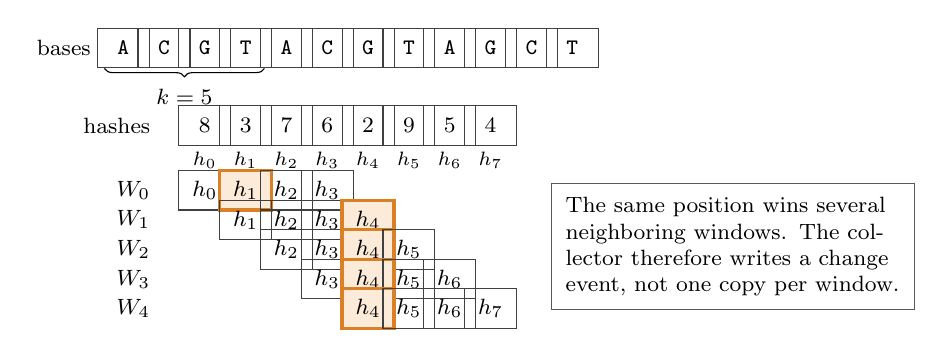
\begin{tikzpicture}[x=.72cm,y=.67cm,font=\footnotesize]
  \foreach \i/\b in {0/A,1/C,2/G,3/T,4/A,5/C,6/G,7/T,8/A,9/G,10/C,11/T}
    \node[rewrite cell,font=\ttfamily\footnotesize] at (.55+\i*.72,4.95) {\b};
  \node[anchor=east] at (.15,4.95) {bases};
  \draw[decorate,decoration={brace,mirror,amplitude=3pt}]
    (.22,4.56)--(3.04,4.56)
    node[midway,below=4pt] {$k=5$};

  \foreach \i/\v in {0/8,1/3,2/7,3/6,4/2,5/9,6/5,7/4}
    \node[rewrite cell] at (1.99+\i*.72,3.48) {\v};
  \node[anchor=east] at (1.20,3.48) {hashes};
  \foreach \i in {0,...,7}
    \node[font=\scriptsize,anchor=north] at (1.99+\i*.72,3.16) {$h_{\i}$};

  \foreach \row/\start/\winner in {0/0/1,1/1/4,2/2/4,3/3/4,4/4/4} {
    \pgfmathsetmacro{\yy}{2.25-.56*\row}
    \node[anchor=east] at (1.20,\yy) {$W_{\row}$};
    \foreach \j in {0,...,3} {
      \pgfmathtruncatemacro{\idx}{\start+\j}
      \pgfmathparse{int(\idx==\winner)}
      \ifnum\pgfmathresult=1
        \node[rewrite min] at (1.99+\idx*.72,\yy) {$h_{\idx}$};
      \else
        \node[rewrite cell] at (1.99+\idx*.72,\yy) {$h_{\idx}$};
      \fi
    }
  }
  \node[rewrite note,text width=4.25cm,anchor=west] at (8.10,1.18)
    {The same position wins several neighboring windows.  The collector
     therefore writes a change event, not one copy per window.};
\end{tikzpicture}
\caption{Minimizer extraction with illustrative $k=5$, $w=4$ hashes.  Each
row is one window of four adjacent $k$-mers. Orange marks the selected
position.  The hash value 2 remains selected while the window moves, so those
windows do not require repeated output.}
\label{fig:rewrite-minimap-walkthrough}
\end{figure}

Equal hashes at different positions are not duplicate records.  The position
and strand make them different candidates.  A complete implementation must
say which equal position is kept as the saved minimum and when the other
positions are written.

\begin{figure}[H]
\centering
\begin{tikzpicture}[font=\footnotesize]
  \node[anchor=west,font=\bfseries] at (0,4.20)
    {(a) Two positions have the same minimum hash};
  \node[anchor=east] at (1.40,3.52) {$W_0$};
  \foreach \i/\v/\sty in {0/8/rewrite cell,1/3/rewrite min,
                            2/7/rewrite cell,3/3/rewrite min}
    \node[\sty] at (1.90+.74*\i,3.52) {\v};
  \node[anchor=west] at (5.05,3.52)
    {hash 3 occurs at two different positions};

  \node[anchor=west,font=\bfseries] at (0,2.62)
    {(b) The next candidate is larger};
  \node[anchor=east] at (1.40,1.94) {$W_1$};
  \foreach \i/\v/\sty in {0/3/rewrite cell,1/7/rewrite cell,
                            2/3/rewrite min,3/9/rewrite new}
    \node[\sty] at (1.90+.74*\i,1.94) {\v};
  \node[rewrite note,text width=5.0cm,anchor=west] at (5.05,1.94)
    {The rightmost 3 remains the saved minimum.  The earlier 3 is still a
     different identity and can require its own event.};

  \draw[rewrite flow] (3.00,1.42) |- (3.95,.72);
  \node[rewrite out,minimum width=1.55cm] at (4.80,.72) {3 at right};
  \node[rewrite out,minimum width=1.70cm] at (6.65,.72) {tied 3 at left};
\end{tikzpicture}
\caption{Why a hash value alone does not define the output.  Both orange
cells have hash 3, but they refer to different $k$-mer positions.  Minimap2
keeps the rightmost equal position as its saved minimum and has explicit
rules for writing other tied identities.}
\label{fig:rewrite-minimap-ties}
\end{figure}

Minimap2 stores the most recent $w$ candidates in a circular array.  It also
stores the current minimum and the array slot containing it.  A normal step
compares the entering candidate with the saved minimum.  A full scan is needed
only when the slot being overwritten contains that saved record.

\begin{figure}[H]
\centering
\begin{tikzpicture}[font=\footnotesize]
  \node[anchor=west,font=\bfseries] at (0,4.55) {(a) Cheap step};
  \node at (2.65,4.12) {before};
  \foreach \i/\v/\sty in {0/8/rewrite cell,1/2/rewrite min,
                            2/7/rewrite cell,3/6/rewrite cell}
    \node[\sty] at (1.55+.72*\i,3.48) {\v};
  \draw[rewrite flow] (4.18,3.48)--(4.82,3.48);
  \node[align=center] at (4.50,2.95) {drop 8\quad add 5};
  \node at (6.25,4.12) {after};
  \foreach \i/\v/\sty in {0/2/rewrite min,1/7/rewrite cell,
                            2/6/rewrite cell,3/5/rewrite new}
    \node[\sty] at (5.18+.72*\i,3.48) {\v};
  \node[rewrite note,text width=3.75cm,anchor=west] at (8.35,3.48)
    {2 is still inside the window. Compare only $5>2$: constant work.};

  \node[anchor=west,font=\bfseries] at (0,2.18) {(b) Expensive step};
  \node at (2.65,1.75) {before};
  \foreach \i/\v/\sty in {0/2/rewrite min,1/7/rewrite cell,
                            2/6/rewrite cell,3/5/rewrite cell}
    \node[\sty] at (1.55+.72*\i,1.10) {\v};
  \draw[rewrite flow] (4.18,1.10)--(4.82,1.10);
  \node[align=center] at (4.50,.58) {drop 2\quad add 9};
  \node at (6.25,1.75) {after};
  \foreach \i/\v in {0/7,1/6,2/5,3/9}
    \node[rewrite new] at (5.18+.72*\i,1.10) {\v};
  \node[rewrite min] at (5.18+.72*2,1.10) {5};
  \draw[draw=rewriteOrange!90!black,very thick]
    (4.80,.72) rectangle (7.72,1.48);
  \node[rewrite note,text width=3.75cm,anchor=west] at (8.35,1.10)
    {2 leaves. Read all $w=4$ live slots and choose 5: $O(w)$.};
\end{tikzpicture}
\caption{The two costs of one minimap2 window advance. Gray cells are already
in the ring, blue is the entering candidate, and orange is the saved or newly
found minimum. A normal step performs one comparison. When the saved minimum
leaves, the algorithm reads the complete window again; this is the rescan.}
\label{fig:rewrite-minimap-rescan}
\end{figure}

\begin{algorithm}[H]
\caption{Scalar minimap2-style rescan, with the output cases stated plainly}
\label{alg:rewrite-minimap-rescan}
\small
\begin{enumerate}
  \item Roll the forward and reverse-complement $k$-mer encodings.  If the
        run is valid and not palindromic, attach the exact minimap-style hash,
        position, and strand. Otherwise use a maximum-valued sentinel.
  \item Write this candidate into the next slot of the $w$-slot ring.
  \item If its hash is less than or equal to the saved minimum, write the old
        saved record when required and save the entering record.
  \item Otherwise, if the overwritten slot held the saved record, write that
        record, scan all $w$ live slots from oldest to newest, and save the
        rightmost record having the smallest hash. Write any other tied
        identities required by the minimap2 rule.
  \item At the end of the sequence, write the remaining saved record.
\end{enumerate}
\end{algorithm}

The selected records become keys in the target index.  Query records with the
same key become candidate anchors.  This downstream use is why a change to the
hash or tie rule cannot be hidden as a local optimization.

\begin{figure}[H]
\centering
\begin{tikzpicture}[font=\footnotesize,node distance=.45cm]
  \node[rewrite box,fill=rewriteGray!14,minimum width=3.15cm] (target)
    {target sequence};
  \node[rewrite box,fill=rewriteBlue!12,minimum width=3.15cm,
        right=1.00cm of target] (query) {query sequence};
  \node[rewrite box,below=.70cm of target,minimum width=3.15cm] (ts)
    {target minimizers $(h,p,z)$};
  \node[rewrite box,below=.70cm of query,minimum width=3.15cm] (qs)
    {query minimizers $(h,p,z)$};
  \node[rewrite box,below=.80cm of ts,minimum width=3.15cm,
        fill=rewriteGray!14] (index) {hash $\rightarrow$ target positions};
  \node[rewrite box,below=.80cm of qs,minimum width=3.15cm,
        fill=rewriteGreen!14] (hits) {matching hashes become anchors};
  \draw[rewrite flow] (target)--(ts);
  \draw[rewrite flow] (query)--(qs);
  \draw[rewrite flow] (ts)--(index);
  \draw[rewrite flow] (qs)--(hits);
  \draw[rewrite flow] (index.east)-|(hits.west);
\end{tikzpicture}
\caption{How minimizer records are used. The target sketch is stored by hash.
The query sketch probes those keys, and matching target/query positions become
anchors. Target and query must therefore use the same candidate hash, tie
rule, strand encoding, and invalid-base rule.}
\label{fig:rewrite-seed-index}
\end{figure}

\section{Naive SIMD rescan: one lane can make every lane scan}
\label{sec:rewrite-naive-simd}

A SIMD lane is one numbered element of a vector register.  The past direct
SIMD port split the sequence into several far-apart pieces and assigned one
piece to each lane.  Every lane kept its own saved minimum, but the processor
executed one shared instruction sequence for the complete lane group.

BioSeq expresses these operations through Highway.  There is no separate
handwritten processor-specific version of this algorithm.  Highway chooses a
supported target and lane count when the program is built or dispatched; the
algorithm below remains the same.

\begin{figure}[H]
\centering
\begin{tikzpicture}[font=\footnotesize]
  \node[anchor=west,font=\bfseries] at (0,7.00)
    {(a) Four far-apart sequence pieces feed four lanes};
  \foreach \i/\fillc in {0/rewriteGray!16,1/rewriteBlue!12,
                           2/rewriteOrange!12,3/rewriteGreen!12} {
    \draw[fill=\fillc] (.40+2.65*\i,6.05) rectangle (2.90+2.65*\i,6.70);
    \node at (1.65+2.65*\i,6.38) {piece \i};
    \draw[rewrite flow] (1.65+2.65*\i,6.02)--(1.65+2.65*\i,5.45);
  }
  \draw[thick] (1.05,4.72) rectangle (10.20,5.35);
  \foreach \x in {3.3375,5.625,7.9125}
    \draw (\x,4.72)--(\x,5.35);
  \foreach \i in {0,...,3}
    \node at (2.19+2.2875*\i,5.04) {lane \i};

  \node[anchor=west,font=\bfseries] at (0,4.08)
    {(b) Lane 0 loses its minimum; the shared branch scans all lanes};
  \foreach \r/\lab in {0/lane 0,1/lane 1,2/lane 2,3/lane 3}
    \node[anchor=east] at (1.35,3.35-.48*\r) {\lab};
  \foreach \r/\c/\v in {
      0/0/7,0/1/6,0/2/5,0/3/9,
      1/0/3,1/1/7,1/2/6,1/3/5,
      2/0/8,2/1/1,2/2/4,2/3/6,
      3/0/5,3/1/6,3/2/2,3/3/8}
    \node[rewrite new] at (1.80+.70*\c,3.35-.48*\r) {\v};
  \node[rewrite min] at (1.80+.70*2,3.35) {5};
  \node[rewrite box,minimum width=2.45cm] (mask) at (6.10,2.63)
    {expiry mask\\$[1,0,0,0]$};
  \draw[rewrite flow] (4.28,2.63)--(mask.west);
  \node[rewrite note,text width=4.0cm,anchor=west] at (7.55,2.63)
    {Only lane 0 accepts a replacement. The processor still loads and
     compares all four vector slots.};
  \draw[draw=rewriteOrange!90!black,very thick]
    (1.43,1.25) rectangle (4.24,3.72);
  \node[rewrite box,fill=rewriteOrange!12,minimum width=4.0cm]
    at (5.95,.62) {$w=4$ vector loads and comparisons};
\end{tikzpicture}
\caption{Why direct SIMD rescan is costly. Each lane follows a different
sequence piece. A nonzero expiry mask enters one shared loop over all $w$
vector slots. Masking protects lanes 1--3 from changing their answers, but it
does not remove their loads and comparisons.}
\label{fig:rewrite-naive-simd-rescan}
\end{figure}

If one lane needs a rescan with probability about $1/w$, then a group of $L$
independent lanes enters the shared slow path with probability
\[
  1-\left(1-\frac1w\right)^L.
\]
For $w=10$ and $L=4$, this is about $34.4\%$.  The vector code still computes
correct lane-local answers, but the expensive branch is taken much more often
than in one scalar stream.

\begin{table}[H]
\centering
\small
\begin{tabularx}{\linewidth}{p{.20\linewidth}XX}
\toprule
Method & What happens when one candidate enters & Why it matters here \\
\midrule
Saved minimum plus rescan & Compare once; scan all $w$ slots only when the
saved record leaves & Excellent scalar common case; one expiring SIMD lane
starts shared work \\
Monotone deque & Remove expired records at the front and larger records at the
back & The number of removals depends on the hash values \\
Prefix and suffix minima & Rebuild a fixed block summary every $w$ steps and
combine two saved values per crossing window & The instruction schedule
depends on the step number, not on which lane contains the minimum \\
\bottomrule
\end{tabularx}
\caption{Three ways to maintain a sliding minimum. The next section uses the
third method because every lane performs the same fixed steps.}
\label{tab:rewrite-sliding-minimum-methods}
\end{table}

\section{SIMD-Minimizers}
\label{sec:rewrite-sea-simd-minimizers}

The SIMD-Minimizers algorithm, published at SEA 2025, makes two linked changes
\cite{groot_koerkamp_simd_minimizers_2025}.  First, each lane follows one
far-apart part of the sequence and advances a rolling ntHash.  Second, window
minima are calculated from fixed-size prefix and suffix summaries.  This is a
different seed definition from minimap2: the hash and equal-minimum rule are
part of the paper algorithm, not transparent replacements for minimap2's
rules.

\subsection{One window minimum from two saved values}

Split the hash stream into blocks of $w$ values.  Within each block, let
$P_i$ be the smallest value from the block start through position $i$, and let
$Q_i$ be the smallest value from position $i$ through the block end.  A window
starting at $j$ and ending at $e=j+w-1$ crosses one block boundary and has
minimum
\[
  \min(Q_j,P_e).
\]
The suffix values are rebuilt in a fixed $w$-step loop at every block
boundary.  Their calculation does not wait for a previously selected value to
leave.

\begin{figure}[H]
\centering
\begin{tikzpicture}[x=.73cm,y=.72cm,font=\footnotesize]
  \node[anchor=east] at (1.15,3.55) {hashes};
  \foreach \i/\v in {0/8,1/5,2/7,3/2,4/9,5/6,6/3,7/4}
    \node[rewrite cell] at (1.60+.73*\i,3.55) {\v};
  \draw[draw=rewriteGray!90!black,very thick]
    (1.25,3.17) rectangle (4.14,3.93);
  \draw[draw=rewriteBlue!90!black,very thick]
    (4.17,3.17) rectangle (7.06,3.93);
  \node[rewriteGray!90!black] at (2.70,4.28) {previous block};
  \node[rewriteBlue!90!black] at (5.62,4.28) {current block};

  \node[anchor=east] at (1.15,2.22) {suffix $Q_i$};
  \foreach \i/\v in {0/2,1/2,2/2,3/2}
    \node[rewrite old] at (1.60+.73*\i,2.22) {\v};
  \node[anchor=east] at (4.98,1.02) {prefix $P_i$};
  \foreach \i/\v in {4/9,5/6,6/3,7/3}
    \node[rewrite new] at (1.60+.73*\i,1.02) {\v};

  \draw[draw=rewriteOrange!90!black,very thick]
    (1.94,3.06) rectangle (4.50,4.04);
  \node[rewrite min] (leftmin) at (2.33,2.22) {2};
  \node[rewrite min] (rightmin) at (4.52,1.02) {9};
  \node[rewrite out,minimum width=4.15cm,align=center] (result)
    at (8.95,.05) {$\min(Q_1,P_4)=\min(2,9)=2$};
  \draw[rewrite flow] (leftmin.south) |- (result.west);
  \draw[rewrite flow] (rightmin.south) |- (result.north);
  \node[rewrite note,text width=4.5cm,anchor=west] at (7.35,3.30)
    {The window has $w=4$ values. Its left part is summarized by one suffix;
     its right part is summarized by one prefix.};
\end{tikzpicture}
\caption{Prefix/suffix minimum for one crossing window. Gray is the earlier
block, blue is the current block, and orange marks the two summary values read
for this window. The answer needs one comparison after the summaries have
been built.}
\label{fig:rewrite-sea-two-stack}
\end{figure}

\subsection{Eight far-apart streams and rolling ntHash}

The paper divides the sequence into eight overlapping logical streams.  Here
``logical stream'' means one independently advanced part of the input; it
does not mean one particular hardware register.  A Highway target exposing
four 32-bit lanes uses two registers for the eight streams, while an
eight-lane target uses one.  Neighboring streams read enough repeated context
to finish windows at their joins.

For each stream, the forward and reverse ntHash states advance by rotations
and exclusive-or operations.  The canonical paper hash is the wrapping sum of
the two states.  The important algorithmic point is that one update reuses the
previous $k$-mer state; it does not rebuild all $k$ bases at each position
\cite{nthash_2016}.

The published pseudocode updates its rolling state with one-bit rotations and
a fixed lookup table for the four DNA letters. When it packs a candidate for
the minimum calculation, it keeps the
upper 16 bits of the 32-bit hash and uses the lower 16 bits for the position
inside the input piece. Thus the minimum comparison sees 16 hash bits, not all
32. In the simple forward-only method, packing the position this way makes an
earlier occurrence win when those hash bits are equal.

When the complete span length $\ell=k+w-1$ is odd, the paper's canonical
method is reverse-complement safe and does more work for an equal minimum. It
remembers the left and right candidate endpoints and counts G/T bases against
A/C bases over the complete span. More G/T chooses the leftmost minimum;
otherwise it chooses the rightmost minimum. Because $\ell$ is odd, the two
counts cannot tie. The method still produces exactly one selected position
for a window. The next output step removes repetitions of that position
across neighboring windows.

\begin{figure}[H]
\centering
\begin{tikzpicture}[font=\footnotesize]
  \node[anchor=west,font=\bfseries] at (0,6.55)
    {(a) Eight far-apart logical streams};
  \draw[thick] (.40,5.62) rectangle (12.40,6.22);
  \foreach \i in {1,...,7}
    \draw[rewriteGray!80] (.40+1.50*\i,5.62)--(.40+1.50*\i,6.22);
  \foreach \i in {0,...,7}
    \node at (1.15+1.50*\i,5.92) {$C_{\i}$};
  \foreach \i in {1,...,7}
    \draw[draw=rewriteOrange!90!black,thick]
      ({.40+1.50*\i-.24},6.27) rectangle
      ({.40+1.50*\i+.24},6.48);
  \node[anchor=west,rewriteOrange!90!black] at (12.65,6.38)
    {repeated context};

  \node[anchor=west,font=\bfseries] at (0,4.88)
    {(b) A Highway target maps those streams to its physical lanes};
  \node[rewrite box,fill=rewriteBlue!14,minimum width=5.20cm] at (3.25,4.10)
    {register group 0: $C_0,C_1,C_2,C_3$};
  \node[rewrite box,fill=rewriteBlue!14,minimum width=5.20cm] at (9.05,4.10)
    {register group 1: $C_4,C_5,C_6,C_7$};

  \node[anchor=west,font=\bfseries] at (0,3.32)
    {(c) The same fixed work is applied to every stream};
  \node[rewrite box,minimum width=2.25cm] (input) at (1.55,2.46)
    {next bases};
  \node[rewrite box,minimum width=2.45cm,text width=2.05cm,
        fill=rewriteBlue!12] (hash)
    at (4.38,2.46) {roll forward and reverse ntHash};
  \node[rewrite box,minimum width=2.35cm,text width=1.95cm] (prefix)
    at (7.22,2.46) {update the block prefix};
  \node[rewrite box,minimum width=2.35cm,text width=1.95cm] (suffix)
    at (10.02,2.46) {fixed suffix rebuild at wrap};
  \node[rewrite box,minimum width=2.25cm,text width=1.85cm,
        fill=rewriteOrange!14] (minimum)
    at (12.75,2.46) {combine one prefix and suffix};
  \draw[rewrite flow] (input)--(hash);
  \draw[rewrite flow] (hash)--(prefix);
  \draw[rewrite flow] (prefix)--(suffix);
  \draw[rewrite flow] (suffix)--(minimum);

  \node[rewrite note,text width=11.8cm,anchor=west] at (.55,.88)
    {A lane means a far-apart stream in this algorithm.  It does not mean the
     next neighboring window.  That distinction is the key difference from
     the current adjacent-window routine described later.};
\end{tikzpicture}
\caption{Input layout and fixed work in SIMD-Minimizers. Eight
overlapping sequence pieces form eight independent logical streams. Highway
may use one or more physical vectors to hold them. Each stream rolls ntHash,
updates a prefix, and uses the fixed suffix schedule.}
\label{fig:rewrite-sea-streams}
\end{figure}

The paper uses two different matrix rearrangements, at two different times.
The first rearrangement happens before hashing: packed input words from
far-apart sequence pieces are rearranged so one SIMD vector contains the next
input word for every piece.  It only prepares input; it removes nothing.

The second rearrangement happens after window minima have been calculated.
At first, one SIMD vector contains the selected positions for several
far-apart streams at the same step.  After several steps, the paper
rearranges that output matrix so one row contains consecutive windows from
one stream.  Consecutive windows often select the same position.  Once those
positions are adjacent in a row, the paper compares neighbors and keeps only
positions that changed.  Finally, when the ordered stream results are joined,
it removes the repeated boundary position caused by the overlapping input
pieces.  This is the paper's output duplicate-removal step.  Equal hash values
at different positions are different records and must remain.

\begin{figure}[H]
\centering
\begin{tikzpicture}[font=\footnotesize]
  \node[font=\bfseries] at (2.30,4.55) {before: one row per vector step};
  \foreach \r/\c/\v in {0/0/1,0/1/12,0/2/23,0/3/30,
                          1/0/1,1/1/13,1/2/23,1/3/35,
                          2/0/2,2/1/13,2/2/23,2/3/35,
                          3/0/4,3/1/13,3/2/23,3/3/36}
    \node[rewrite cell] at (.95+.72*\c,3.80-.56*\r) {\v};

  \node[rewrite box,minimum width=1.65cm,text width=1.35cm] (swap)
    at (5.20,2.95) {rows become columns};
  \draw[rewrite flow] (3.82,2.95)--(swap.west);
  \draw[rewrite flow] (swap.east)--(6.55,2.95);

  \node[font=\bfseries] at (8.10,4.55) {after: one row per stream};
  \foreach \r/\c/\v in {0/0/1,0/1/1,0/2/2,0/3/4,
                          1/0/12,1/1/13,1/2/13,1/3/13,
                          2/0/23,2/1/23,2/2/23,2/3/23,
                          3/0/30,3/1/35,3/2/35,3/3/36}
    \node[rewrite cell] at (7.02+.72*\c,3.80-.56*\r) {\v};

  \node[rewrite box,minimum width=2.20cm,text width=1.90cm,
        fill=rewriteGreen!13] (dedup)
    at (11.55,2.95) {keep a position only when it changes};
  \draw[rewrite flow] (9.92,2.95)--(dedup.west);

  \node[rewrite out,minimum width=3.20cm] at (2.30,.84)
    {stream 0: 1, 2, 4};
  \node[rewrite out,minimum width=3.20cm] at (5.80,.84)
    {stream 1: 12, 13};
  \node[rewrite out,minimum width=3.20cm] at (9.30,.84)
    {stream 3: 30, 35, 36};
\end{tikzpicture}
\caption{The paper's output rearrangement and duplicate removal. Before the
rearrangement, each row is one SIMD step across far-apart streams. Afterwards,
each row is a sequence of neighboring windows from one stream, such as
$[1,1,2,4]$. Comparing adjacent positions reduces that row to $[1,2,4]$.
After the stream rows are joined, one further boundary comparison removes an
identical position produced on both sides of an overlap. The earlier input
rearrangement is a separate operation and removes nothing.}
\label{fig:rewrite-sea-output-reorder}
\end{figure}

\section{How BioSeqDB reached V8 and what happened afterward}
\label{sec:rewrite-version-history}

The old version labels are useful, but they are not the names of fifteen
successive user-selectable algorithms.  Two experiment logs reused some of
the same numbers, and several later versions changed chaining or divergence
estimation rather than minimizer extraction.  The sequence below therefore
states what actually changed instead of treating every number as a new
collector.

\subsection{The direct-rescan line}

V1 repaired a correctness error in the first direct SIMD collector.  The
strand value had effectively been written as zero for every emitted record,
so reverse-oriented seeds were mishandled.  The fix carried one strand value
beside every hash through ordinary updates and rescans.  The window algorithm
itself was still the shared SIMD rescan from
Figure~\ref{fig:rewrite-naive-simd-rescan}.

V2 made that same algorithm cheaper for DNA4 by replacing general complement
lookups with the two-bit complement operation and by simplifying masks.  V3
read packed input more directly and changed surrounding code.  Neither V2 nor
V3 changed when a rescan occurred.

The labels V4--V6 are ambiguous in the retained experiment history.  One
table reused V1--V6 for small two-stack edits: remove unused delay state, pack
the strand bit with a saved word, remove a third ring, add branch hints,
unroll the fixed $w=10$ loop, and repair a wrap case.  Other prose calls the
naive direct collector ``V6.''  These were local experiments, not three
separate public algorithms.  The reliable conclusion is the one already
shown in Section~\ref{sec:rewrite-naive-simd}: improving masks and storage did
not remove the shared, value-triggered $w$-slot scan.

\subsection{The prefix/suffix line}

One earlier experiment already had the prefix/suffix minimum structure.  V7
inlined the packed forward and reverse-complement update and made the $k=15$
shifts compile-time constants.  V8 kept the prefix/suffix structure and
postponed the full minimap-style integer mix until a record was emitted.  That
saved work, but it was not a behavior-preserving optimization:
the cheaper value used inside the window could choose a different $k$-mer.
The label V8.5 was used when a golden-ratio multiplication was added to this
inside-window ordering key.  The old snapshot discussed in the next section
contains that multiplied key.

V9 replaced a generic iterator and captured callback with a hand-written
input/matrix loop.  V10 did not add another minimizer algorithm; it paired the
V9 collector with a downstream reverse-chain estimator change and small
instruction reductions.  The estimator change was later removed.

V11 advanced two independent groups of Highway lanes together.  The two
groups still followed distant input pieces and used the same prefix/suffix
rule; their independent state merely gave the processor other work while one
group waited on a dependent operation.  V12 moved the per-base body into a
named, forced-inline function after the captured callback remained an actual
call.  V12 also removed palindrome filtering.  That changes behavior in
general, although a reverse-complement palindrome is impossible for the
admitted odd length $k=15$ over DNA4.

\subsection{Versions that changed later stages or were rejected}

V13 retained the V12 minimizer and replaced a downstream sort and repeated
binary searches with a prefix-count array.  It was an alignment-pipeline
change, not a new way to calculate a window minimum.  Two attempted reductions
of the minimizer state in this period were reverted after they discarded too
many hash bits.

V14 tried a separate rolling-ntHash ordering collector.  It changed which
minimizers were selected and was not kept as the production route.  The
current bounded ntHash selector described later is a different implementation
with its own stored hash and tie rules; it is not V14 under a new name.  V15
changed SIMD chaining, not minimizer extraction, and the attempted dual-batch
chainer was not retained as the production choice.

\begin{table}[H]
\centering
\footnotesize
\begin{tabularx}{\linewidth}{p{.13\linewidth}p{.32\linewidth}X}
\toprule
Label & Main change & What it means for the minimizer algorithm \\
\midrule
V1 & carry the strand through every SIMD state update & correctness repair;
direct rescan unchanged \\
V2--V3 & cheaper DNA4 complement/masks and direct packed input & less
bookkeeping; direct rescan unchanged \\
V4--V6 & reused labels for small two-stack edits; ``V6'' also names the naive
collector & not three uniquely recoverable public algorithms \\
V7 & inline packed rolling state; constant $k=15$ shifts & performance-only
preparation for the prefix/suffix collector \\
V8, V8.5 & prefix/suffix minima; delay the full mix; add the multiplied
ordering key & removes expiry-triggered rescans but changes the selected seed
rule \\
V9 & hand-written input and matrix loop & same V8.5 seed rule, less iterator
and callback work \\
V10 & downstream estimator experiment plus small V9 edits & no new minimizer
kernel \\
V11 & two independent Highway lane groups & same per-lane algorithm, more
independent work in flight \\
V12 & force the per-base body inline; remove palindrome check & faster call
shape; palindrome change is semantic outside admitted odd-$k$ DNA4 \\
V13 & downstream prefix-count estimator & no new minimizer kernel \\
V14 & separate rolling-ntHash ordering experiment & different seed selection;
not retained as production \\
V15 & dual-batch chaining experiment & not a minimizer change \\
\bottomrule
\end{tabularx}
\caption{Plain history of the old version labels.  The table separates
changes to minimizer extraction from changes to later alignment stages and
states where the retained labels were reused.}
\label{tab:rewrite-version-history}
\end{table}

None of these old function variants is a current user selector.  Cleanup work
kept the V12/V13-era collector under one name, and later work produced the two
current CPU routes described in Section~\ref{sec:rewrite-current-bioseq}.

\section{Past V8: the same minimum structure, but not SIMD-Minimizers}
\label{sec:rewrite-v8}

Past V8 adopted the paper's useful way of finding window minima: each lane
followed a far-apart input piece, every lane kept prefix and suffix summaries,
and the suffix pass ran on a fixed schedule.  The complete algorithm was still
different.  V8 selected with a cheaper key derived from the canonical packed
$k$-mer, deferred the full minimap-style scramble until output, resolved an
equal key with its packed local position, and appended selected lanes through
a scalar loop.  It did not implement the paper's output transpose and
cross-stream join removal.  Its ring and summaries were fixed arrays; no
\texttt{std::map} was part of the minimum calculation.

The inspected V8 snapshot also contains two representation errors, separate
from the intended algorithm.  For the usual 32-bit, $k=15$ form, the mask used
for the multiplied ordering key retains only fourteen useful hash bits.  In a
64-bit instantiation of the same expression, its two masks do not overlap and
the ordering hash becomes zero.  The code also stores strand in the low bit of
the packed canonical word and clears that bit before calculating the emitted
minimap-style hash.  A word whose original low bit was one therefore receives
the wrong emitted hash.  These errors are additional reasons not to treat V8
output as an exact minimap2 stream; they are not properties of the
prefix/suffix method itself.

\begin{figure}[H]
\centering
\begin{tikzpicture}[font=\footnotesize]
  \node[anchor=west,font=\bfseries] at (0,8.10)
    {(a) One V8 lane follows one far-apart, overlapping input piece};
  \foreach \r/\x in {0/.65,1/2.25,2/3.85,3/5.45} {
    \pgfmathsetmacro{\yy}{7.38-.52*\r}
    \node[anchor=east] at (.48,\yy) {lane \r};
    \draw[fill=rewriteGray!20] (\x,\yy-.22) rectangle (\x+.72,\yy+.22);
    \draw[fill=rewriteBlue!14,draw=rewriteBlue!90!black]
      (\x+.72,\yy-.22) rectangle (\x+2.32,\yy+.22);
  }
  \node[rewrite note,text width=4.30cm,anchor=west] at (8.05,6.62)
    {Neighboring lanes read some of the same bases. Their minimum state does
     not cross the lane boundary.};

  \node[anchor=west,font=\bfseries] at (0,5.12)
    {(b) SIMD calculates four independent window minima};
  \foreach \r/\lab in {0/L0,1/L1,2/L2,3/L3}
    \node[anchor=east] at (1.05,4.43-.48*\r) {\lab};
  \foreach \r/\c/\v in {
      0/0/9,0/1/4,0/2/7,0/3/2,
      1/0/8,1/1/3,1/2/6,1/3/5,
      2/0/6,2/1/1,2/2/8,2/3/4,
      3/0/7,3/1/5,3/2/2,3/3/6}
    \node[rewrite cell] at (1.48+.67*\c,4.43-.48*\r) {\v};
  \foreach \r/\c/\v in {0/3/2,1/1/3,2/1/1,3/2/2}
    \node[rewrite min] at (1.48+.67*\c,4.43-.48*\r) {\v};
  \node[rewrite box,minimum width=2.35cm,text width=1.95cm] (fixed)
    at (5.60,3.72) {fixed prefix/suffix combine};
  \draw[rewrite flow] (4.02,3.72)--(fixed.west);
  \foreach \r/\v in {0/2,1/3,2/1,3/2}
    \node[rewrite min] at (7.34,4.43-.48*\r) {\v};
  \node[rewrite note,text width=4.15cm,anchor=west] at (7.95,3.72)
    {The minimum update is vectorized. The branch is controlled by the shared
     step counter, not by a lane's hash.};

  \node[anchor=west,font=\bfseries] at (0,2.02)
    {(c) Sparse output returns to scalar lane handling};
  \node[rewrite box,minimum width=2.30cm,text width=1.95cm] (store)
    at (2.00,.74) {store hash, position, strand, and mask};
  \node[rewrite box,minimum width=2.25cm,text width=1.90cm] (loop)
    at (5.00,.74) {scalar loop over lane 0 to lane 3};
  \node[rewrite out,minimum width=1.65cm] at (8.00,1.09) {lane 1 record};
  \node[rewrite out,minimum width=1.65cm] at (8.00,.37) {lane 3 record};
  \draw[rewrite flow] (store)--(loop);
  \draw[rewrite flow] (loop.east)-|(7.05,1.09);
  \draw[rewrite flow] (loop.east)-|(7.05,.37);
  \node[rewrite note,text width=3.6cm,anchor=west] at (9.10,.74)
    {Only repetition within one lane is suppressed. Overlap records from two
     neighboring lanes can remain.};
\end{tikzpicture}
\caption{Past V8 lane processing. Input lanes are far apart, the
prefix/suffix minimum is calculated with SIMD operations, and sparse records
are appended by a scalar lane loop. V8 has an input rearrangement for distant
pieces, but it has no SIMD-Minimizers output rearrangement and join removal.}
\label{fig:rewrite-v8-lanes}
\end{figure}

\begin{table}[H]
\centering
\footnotesize
\begin{tabularx}{\linewidth}{p{.18\linewidth}XX}
\toprule
Question & SIMD-Minimizers & Past V8 \\
\midrule
What is one lane? & One of eight far-apart, overlapping input streams & One
far-apart, overlapping input piece \\
How is the hash advanced? & Rolling forward and reverse ntHash & Rolling
canonical packed word with a cheaper multiplied ordering key; full
minimap-style mix delayed until output \\
How is the minimum found? & Block prefixes and suffixes & The same
prefix/suffix minimum structure \\
How is an equal minimum chosen? & For an odd complete span, more G/T than A/C
selects the leftmost occurrence; otherwise the rightmost occurrence is
selected & Packed local position selects one earlier equal key;
complete minimap2 tie events are not reproduced \\
How is output collected? & Rearrange vector-step output into stream rows and
remove repeated join identities & Store vectors, inspect lanes in scalar code,
and suppress repetition only within a lane \\
Is a tree map used? & No & No \\
\bottomrule
\end{tabularx}
\caption{The shared prefix/suffix minimum does not make V8 and SIMD-Minimizers the
same complete algorithm. Their hash, equal-minimum rule, and output handling
differ.}
\label{tab:rewrite-sea-v8-differences}
\end{table}

\section{Current BioSeq algorithms and the route selected by the benchmark}
\label{sec:rewrite-current-bioseq}

The public name
\begin{center}
\footnotesize
\texttt{bioseq\_block\_simd\_dp\_}\\
\texttt{two\_stack\_nthash\_no\_index}
\end{center}
preserves names from earlier development.  Static routing is more specific:
the named large no-index case maps target pieces and the query through the
state-carrying adjacent-window SIMD routine.  Its active window-minimum loop
does not call the separate whole-input prefix/suffix routine and does not call
the bounded rolling-ntHash routine.  The phrase \emph{adjacent-window
routine} is used below because lane~0 handles one window, lane~1 handles the
very next window, and so on.

\begin{figure}[H]
\centering
\begin{tikzpicture}[font=\footnotesize]
  \node[rewrite box,minimum width=7.25cm,fill=rewriteGray!15] (name)
    at (6.30,6.35)
    {named E2E row:\\
     \texttt{bioseq\_block\_simd\_dp\_}\\
     \texttt{two\_stack\_nthash\_no\_index}};
  \node[rewrite box,minimum width=4.20cm] (select) at (6.30,5.05)
    {public selector \texttt{TWO\_STACK\_NTHASH}\\chooses the exact SIMD family};
  \draw[rewrite flow] (name)--(select);

  \node[rewrite box,minimum width=4.25cm,fill=rewriteBlue!12] (target)
    at (3.20,3.45) {each target segment\\state carried to the next segment};
  \node[rewrite box,minimum width=4.25cm,fill=rewriteBlue!12] (query)
    at (9.40,3.45) {query sketch\\same exact seed rules};
  \draw[rewrite flow] (select.south) |- (target.north);
  \draw[rewrite flow] (select.south) |- (query.north);

  \node[rewrite box,minimum width=5.15cm,fill=rewriteOrange!14] (adj)
    at (6.30,1.90) {adjacent-window SIMD block\\exact minimap-style hash and ties};
  \draw[rewrite flow] (target.south) |- (adj.west);
  \draw[rewrite flow] (query.south) |- (adj.east);

  \node[rewrite note,text width=4.45cm,anchor=west,fill=rewriteGray!10]
    at (.35,.35) {Not selected here: whole-input \texttt{vector\_stream}
    two-stack control.};
  \node[rewrite note,text width=4.45cm,anchor=west,fill=rewriteGray!10]
    at (7.85,.35) {Not selected here: bounded rolling-ntHash scheme.};
\end{tikzpicture}
\caption{What the named no-index E2E row actually runs. Both target segments
and the query use the state-carrying adjacent-window SIMD routine. The
words ``two stack'' and ``nthash'' in the public row name do not describe the
active inner minimum or hash in this route.}
\label{fig:rewrite-current-e2e-route}
\end{figure}

\subsection{The adjacent-window calculation}

Let $B$ be the number of candidate positions handled together.  The routine
retains the last $k-1$ bases and the last $w-1$ candidate records.  It adds $B$
new consecutive bases, forms $B$ consecutive $k$-mers, calculates the exact
minimap-style hash for each, and places the retained and new candidates next
to one another.  It then makes $w$ shifted SIMD loads.  Lane $j$ is the whole
window beginning at the $j$th candidate, so lanes are neighboring windows in
this routine.  This is the opposite of V8, where lanes are far-apart input
pieces.

\begin{figure}[H]
\centering
\begin{tikzpicture}[font=\footnotesize]
  \node[anchor=west,font=\bfseries] at (0,9.05)
    {(a) Retained context plus $B$ new consecutive positions};
  \node[rewrite box,minimum width=4.0cm,fill=rewriteGray!18] (basesold)
    at (2.35,8.28) {last $k-1$ bases};
  \node[rewrite box,minimum width=2.40cm,fill=rewriteBlue!14] (basesnew)
    at (5.75,8.28) {$B$ new bases};
  \node[rewrite box,minimum width=4.05cm] (make) at (9.65,8.28)
    {$B$ consecutive canonical $k$-mers\\and exact minimap-style hashes};
  \draw[rewrite flow] (basesold.east)--(basesnew.west);
  \draw[rewrite flow] (basesnew.east)--(make.west);

  \node[anchor=west,font=\bfseries] at (0,7.28)
    {(b) Four neighboring windows are calculated together ($B=4,w=4$ shown)};
  \node[anchor=east] at (1.78,6.58) {candidate row};
  \foreach \i/\v/\sty in {0/7/rewrite old,1/6/rewrite old,2/5/rewrite old,
                            3/9/rewrite new,4/4/rewrite new,5/8/rewrite new,
                            6/3/rewrite new}
    \node[\sty] at (2.20+.70*\i,6.58) {\v};

  \foreach \r/\lab in {0/$W_0$,1/$W_1$,2/$W_2$,3/$W_3$}
    \node[anchor=east] at (1.78,5.82-.54*\r) {\lab};
  \foreach \r/\c/\v in {
      0/0/7,0/1/6,0/2/5,0/3/9,
      1/0/6,1/1/5,1/2/9,1/3/4,
      2/0/5,2/1/9,2/2/4,2/3/8,
      3/0/9,3/1/4,3/2/8,3/3/3}
    \node[rewrite cell] at (2.20+.70*\c,5.82-.54*\r) {\v};
  \foreach \r/\c/\v in {0/2/5,1/3/4,2/2/4,3/3/3}
    \node[rewrite min] at (2.20+.70*\c,5.82-.54*\r) {\v};

  \node[rewrite box,minimum width=2.45cm] (reduce) at (6.38,5.02)
    {$w$ shifted loads\\and $\leq$ reduction};
  \draw[rewrite flow] (5.02,5.02)--(reduce.west);
  \foreach \r/\v in {0/5,1/4,2/4,3/3}
    \node[rewrite min] at (8.32,5.82-.54*\r) {\v};
  \node[rewrite note,text width=3.80cm,anchor=west] at (8.92,5.02)
    {One lane is one complete window. The next lane is the window one
     candidate position to the right.};

  \node[anchor=west,font=\bfseries] at (0,3.15)
    {(c) The ordinary output path writes only changed selections};
  \node[anchor=east] at (1.93,2.45) {previous};
  \node[anchor=east] at (1.93,1.88) {current};
  \node[anchor=east] at (1.93,1.31) {write?};
  \foreach \i/\v in {0/5@3,1/5@3,2/4@5,3/4@5}
    \node[rewrite old,minimum width=.93cm] at (2.48+.98*\i,2.45) {\v};
  \foreach \i/\v in {0/5@3,1/4@5,2/4@5,3/3@7}
    \node[rewrite new,minimum width=.93cm] at (2.48+.98*\i,1.88) {\v};
  \foreach \i/\v in {0/0,1/1,2/0,3/1}
    \node[rewrite cell,minimum width=.93cm] at (2.48+.98*\i,1.31) {\v};
  \node[rewrite box,minimum width=2.35cm,fill=rewriteGreen!13] (compress)
    at (7.45,1.88) {compressed store\\of marked lanes};
  \draw[rewrite flow] (5.95,1.88)--(compress.west);
  \node[rewrite out,minimum width=1.28cm] at (9.55,2.20) {5@3};
  \node[rewrite out,minimum width=1.28cm] at (9.55,1.55) {4@5};
  \node[rewrite note,text width=2.55cm,anchor=west] at (10.35,1.88)
    {3@7 remains saved until a later event.};
\end{tikzpicture}
\caption{The current adjacent-window minimum with small values for
legibility. Gray candidates come from the preceding block and blue candidates
are new. Four lanes hold four neighboring windows. The real $k=15,w=10$
specialization reads ten shifted vectors and produces $B$ window minima.}
\label{fig:rewrite-current-adjacent-windows}
\end{figure}

The comparison uses $\leq$, so a later equal-hash position replaces an earlier
one.  Ordinary changes form one lane mask and are written in a compressed
batch.  Equal hashes at several different positions can require several
records for one window.  That rare case rearranges an event matrix so all
records for $W_0$ precede all records for $W_1$, and so on.  The rearrangement
restores output order; it is not a deduplication pass.

\begin{figure}[H]
\centering
\begin{tikzpicture}[font=\footnotesize]
  \node[font=\bfseries] at (2.45,5.32) {before: one row per event slot};
  \foreach \c/\lab in {0/$W_0$,1/$W_1$,2/$W_2$,3/$W_3$}
    \node at (1.35+.78*\c,4.72) {\lab};
  \foreach \r/\lab in {0/old,1/tie 1,2/tie 2}
    \node[anchor=east] at (.87,4.12-.56*\r) {\lab};
  \foreach \r/\c/\v in {0/0/a,0/1/b,0/2/--,0/3/f,
                          1/0/c,1/1/--,1/2/e,1/3/g,
                          2/0/d,2/1/--,2/2/--,2/3/--}
    \node[rewrite cell] at (1.35+.78*\c,4.12-.56*\r) {\v};

  \node[rewrite box,minimum width=1.85cm] (swap) at (5.60,3.55)
    {rows become\\columns};
  \draw[rewrite flow] (4.28,3.55)--(swap.west);
  \draw[rewrite flow] (swap.east)--(6.83,3.55);

  \node[font=\bfseries] at (9.18,5.32) {after: one row per window};
  \foreach \c/\lab in {0/old,1/tie 1,2/tie 2}
    \node at (8.05+.90*\c,4.72) {\lab};
  \foreach \r/\lab in {0/$W_0$,1/$W_1$,2/$W_2$,3/$W_3$}
    \node[anchor=east] at (7.53,4.12-.56*\r) {\lab};
  \foreach \r/\c/\v in {0/0/a,0/1/c,0/2/d,
                          1/0/b,1/1/--,1/2/--,
                          2/0/--,2/1/e,2/2/--,
                          3/0/f,3/1/g,3/2/--}
    \node[rewrite cell] at (8.05+.90*\c,4.12-.56*\r) {\v};

  \node[rewrite out,minimum width=2.25cm] at (2.10,.85) {a\quad c\quad d};
  \node[rewrite out,minimum width=.85cm] at (3.82,.85) {b};
  \node[rewrite out,minimum width=.85cm] at (4.78,.85) {e};
  \node[rewrite out,minimum width=1.55cm] at (6.02,.85) {f\quad g};
  \node[rewrite note,text width=5.25cm,anchor=west] at (7.05,.85)
    {Every named record remains. Only empty sentinel cells disappear.};
\end{tikzpicture}
\caption{Rare equal-minimum output in the current adjacent-window routine.
The matrix is rearranged to put records in window order. A compressed store
removes empty cells; it does not compare or remove two real records.}
\label{fig:rewrite-current-event-order}
\end{figure}

\subsection{State across input fragments}

A normal storage-fragment boundary does not end the biological sequence.  The
routine retains at most $k-1$ bases, fewer than one incomplete vector group,
$w-1$ candidates, and the selected record of the last complete window.  An
ambiguous base is different: it clears the valid $k$-mer run and advances a
maximum-valued candidate through the window.

\begin{figure}[H]
\centering
\begin{tikzpicture}[font=\footnotesize]
  \draw[fill=rewriteGray!18] (.55,4.55) rectangle (5.35,5.25);
  \node at (2.95,4.90) {packed fragment $f_i$};
  \draw[fill=rewriteBlue!14,draw=rewriteBlue!90!black]
    (7.05,4.55) rectangle (11.85,5.25);
  \node at (9.45,4.90) {packed fragment $f_{i+1}$};
  \draw[rewrite flow] (5.35,4.90)--(7.05,4.90);
  \node[above,align=center] at (6.20,5.05) {storage boundary\\no reset};

  \node[rewrite box,minimum width=11.30cm,fill=rewriteGray!12] (state)
    at (6.20,3.02) {retained state: $k-1$ bases \quad $w-1$ candidates
      \quad incomplete group \quad selected record};
  \draw[rewrite flow] (4.25,4.50)|-(state.north);
  \draw[rewrite flow] (state.north)-|(8.15,4.50);

  \node[rewrite box,minimum width=9.90cm,fill=rewriteOrange!13] (amb)
    at (6.20,1.40) {ambiguous base: clear the valid $k$-mer context and
      insert a maximum-valued candidate};
  \draw[rewrite flow] (state)--(amb);
  \node[rewrite note,text width=10.8cm,anchor=west] at (.80,.20)
    {Only end-of-input performs the final saved-record write. A fragment
     boundary and an ambiguous base therefore have different effects.};
\end{tikzpicture}
\caption{Bounded continuation in the current adjacent-window SIMD path. State is carried
across a normal storage boundary, so a window can cross it without rereading
an overlapping chunk. An ambiguous base resets the valid $k$-mer run but does
not masquerade as end-of-input.}
\label{fig:rewrite-current-continuation}
\end{figure}

\begin{algorithm}[H]
\caption{Current $k=15,w=10$ adjacent-window block, simplified}
\label{alg:rewrite-current-adjacent-block}
\small
\begin{enumerate}
  \item Join retained base context with $B$ new positions and build $B$
        consecutive forward and reverse-complement $k$-mers.
  \item Choose each canonical $k$-mer, mark invalid or palindromic candidates
        with a maximum sentinel, and calculate the exact minimap-style hash.
  \item Join the retained $w-1$ candidate tail with the $B$ new candidates.
        Read $w$ shifted vectors and reduce with $\leq$; lane $j$ now contains
        the minimum of the $j$th neighboring window.
  \item Form masks for a smaller entering value, an expired saved record,
        first-window output, and final output.
  \item On the common path, compressed-store the marked records.  If equal
        hashes at different identities are present, build the tie-event
        matrix, rearrange it into window order, and compressed-store all real
        cells.
  \item Retain the final base context, candidate tail, incomplete group, and
        selected record for the next input fragment.
\end{enumerate}
\end{algorithm}

\subsection{Why this complete route can be faster than V8}

The current minimum operation is not an asymptotically cheaper form of V8's
two-stack minimum.  V8 rebuilds $w$ suffix entries once every $w$ steps.  The
current routine makes $w$ shifted comparisons for every group of $B$ adjacent
windows and also calculates the exact selection hash.  A speed advantage, when
measured, must therefore come from the complete route around that reduction:

\begin{itemize}
  \item new $k$-mers come from one short consecutive input region, rather than
        from an input rearrangement of far-apart pieces;
  \item state crosses ordinary fragments directly, without overlapping lane
        reads and their repeated join records;
  \item the ordinary output is written as one compressed batch rather than by
        visiting every lane in scalar code; and
  \item the larger exact tie calculation runs only after a hash precheck says
        it is needed.
\end{itemize}

Those are code-level reasons, not timing results.  Section
\ref{sec:rewrite-performance-evidence} keeps the older measurements separate
and does not present them as a V8-versus-current measurement.

\subsection{Other current minimizer routes}

BioSeq has several routes because they do not all produce the same seed
stream. In particular, the three values assigned to
\texttt{dispatch.params.minimizer\_algorithm} select three different ways of
making minimizers. They do not select the prefilter, chaining method, or final
alignment method; those are chosen by other fields. The same minimizer setting
is used for the query and target so that a query seed can be found in the
target table.

\subsubsection{What the three ordinary benchmark settings mean}

The ordinary alignment benchmark normally supplies DNA4 packed into 32-bit
words, with the complete query and target already available in memory, and
uses $k=15,w=10$. Under those conditions the three assignments in the
benchmark source mean the following.

\begin{description}
  \item[\texttt{two\_stack\_nthash}.]
    The four \texttt{bioseq\_prefilter\_*} rows and the six ordinary alignment
    rows whose names contain \texttt{two\_stack\_nthash} run the whole-input
    descendant of V8. One lane follows one far-apart part of the sequence. It
    advances packed forward and reverse-complement $k$-mers, updates a prefix
    minimum, and rebuilds suffix minima once every $w$ positions. Long inputs
    advance two independent Highway vector groups. Despite the setting's
    historical name, this route does not calculate ntHash. The E2E caller
    shown earlier uses the same setting but supplies the target as pieces and
    requires exact minimap-style output for its target table, so it
    deliberately selects the adjacent-window algorithm instead.

  \item[\texttt{bounded\_nthash\_simd}.]
    The two ordinary rows whose names contain \texttt{bounded\_nthash} call
    the bounded-input entry point. The query is processed as one range and the
    target as one or more ranges. Every range uses eight logical ntHash
    streams and the prefix/suffix minimum. This is the maintained successor of
    the old \texttt{PAPER\_NTHASH\_SIMD} setting. It is the BioSeq algorithm
    closest to SIMD-Minimizers, but its exact hash and tied-minimum output differ from
    the paper, as explained below.

  \item[\texttt{simd\_minimap2\_reference}.]
    This setting is used by the ordinary slow-reference row. It runs the naive
    SIMD rescan from
    Figure~\ref{fig:rewrite-naive-simd-rescan}. One lane follows one far-apart
    sequence part and saves one minimum. If any lane loses its saved minimum,
    the shared loop reads all $w$ vector slots; masks ensure that only expired
    lanes change their answer.
\end{description}

Words such as \texttt{ksw2}, \texttt{block}, \texttt{prefilter}, or
\texttt{vulkan\_tiled\_dp} elsewhere in an ordinary row name describe later
mapping work. They do not change the minimizer route just described. Highway
chooses the available processor target and physical lane count; there is no
separate handwritten AVX algorithm. If a required input shape is unsupported,
the checked SIMD setting reports failure. It does not silently change to the
scalar minimizer after entering that checked route.

\subsubsection{The whole-input prefix/suffix route}

When \texttt{two\_stack\_nthash} receives one complete, already available
DNA4 sequence stored in 32-bit words with $k=15,w=10$, it can choose the
whole-input descendant of V8.  This is the route reached by the ordinary
in-memory benchmark names that contain \texttt{two\_stack\_nthash}.  Each lane
owns a far-apart sequence piece.  The code shifts packed forward and
reverse-complement words, ranks their canonical word with the multiplied
ordering key, updates a prefix minimum, and rebuilds suffix minima every $w$
steps.  Long inputs advance two independent Highway lane groups together.

This route still does not calculate ntHash.  It applies the minimap-style mix
only when it emits, stores SIMD results to arrays, and then visits output lanes
with scalar code.  It has no state format for continuing through ordinary
input fragments.  For these reasons it cannot be substituted for the
adjacent-window route while a target index and query are being built from
pieces.

\begin{table}[H]
\centering
\footnotesize
\begin{tabularx}{\linewidth}{p{.22\linewidth}p{.22\linewidth}X
  p{.10\linewidth}}
\toprule
Minimizer setting & Input for this row & Actual algorithm & Named
no-index E2E? \\
\midrule
\texttt{scalar} & DNA4 or DNA5 scalar input & saved minimum plus occasional
ring rescan & no \\
\shortstack[l]{\texttt{simd\_minimap2\_}\\\texttt{reference}} &
one complete DNA4 input & distant
lane streams with one saved minimum per lane and a shared SIMD rescan & no \\
\texttt{two\_stack\_nthash} & a target table or input supplied in pieces &
neighboring windows, full $w$-slot SIMD reduction, minimap-style hash & yes \\
\texttt{two\_stack\_nthash} & complete DNA4 stored in 32-bit words,
$k=15,w=10$ &
distant lane streams with V8-descended prefix/suffix minima & no \\
\texttt{bounded\_nthash\_simd} & DNA4 query or bounded target range,
$k=15,w=10$ & eight rolling-ntHash streams with prefix/suffix minima & no \\
\shortstack[l]{\texttt{vulkan\_minimap\_}\\\texttt{integer}} &
supported GPU and input & many GPU
tiles, each using a serial minimap-style ring/rescan & no \\
\bottomrule
\end{tabularx}
\caption{Current minimizer settings and their actual inner algorithms.  The
\texttt{two\_stack\_nthash} selector is the confusing case: its caller and
input shape choose between two different algorithms.}
\label{tab:rewrite-current-routing}
\end{table}

\begin{table}[H]
\centering
\footnotesize
\begin{tabularx}{\linewidth}{p{.40\linewidth}XX}
\toprule
Configured run name or family & Query minimizers & Target minimizers \\
\midrule
\shortstack[l]{Named E2E \texttt{two\_stack\_nthash\_}\\
\texttt{no\_index}} & adjacent-window SIMD &
adjacent-window SIMD while building a temporary target table \\
\shortstack[l]{Named E2E \texttt{two\_stack\_nthash\_}\\
\texttt{just\_index}} & adjacent-window SIMD &
matching adjacent-window target index built before mapping \\
Ordinary \texttt{bioseq\_prefilter\_*} and names containing
\texttt{two\_stack\_nthash} & whole-input V8 descendant & whole-input V8
descendant \\
Ordinary \texttt{simd\_minimap2\_slow} & direct SIMD rescan & direct SIMD
rescan \\
Ordinary names containing \texttt{bounded\_nthash} & bounded rolling ntHash &
bounded rolling ntHash \\
Scalar BioSeq rows & scalar rescan & scalar rescan \\
Vulkan-minimizer rows & Vulkan tile rescan & Vulkan tile rescan or its
device target-index builder \\
External minimap2 rows & bundled minimap2 sketch & bundled minimap2 sketch or
its prebuilt index \\
\bottomrule
\end{tabularx}
\caption{What the configured test families actually execute.  This mapping
comes from the current call paths, not from interpreting a historical word in
the displayed run name.  No current configured run calls the old V8 source
body directly.}
\label{tab:rewrite-configured-routes}
\end{table}

\begin{table}[H]
\centering
\footnotesize
\begin{tabularx}{\linewidth}{p{.19\linewidth}XX}
\toprule
Question & Past V8 & Current adjacent-window E2E path \\
\midrule
What is one lane? & One far-apart, overlapping input piece & One of the next
$B$ neighboring windows \\
How is input prepared? & Rearrange packed input so every lane receives the
next base of its own piece & Read consecutive bases and retain $k-1$ bases
across input pieces \\
How is the minimum found? & Update a prefix; rebuild suffixes once per $w$
steps; compare one prefix and suffix & Read $w$ shifted vectors and reduce
each of $B$ complete windows \\
Which hash selects it? & Cheaper multiplied ordering key; full minimap-style
mix delayed until output & Exact minimap-style hash before selection \\
How are normal records written? & Store vectors and inspect lanes in scalar
code & One event mask and one compressed SIMD store \\
What is rearranged? & Input values for far-apart pieces & Rare equal-minimum
output records, solely to restore window order \\
Is there a deduplication pass? & No; suppression is within one lane & No;
unchanged selections are suppressed before output and real ties remain \\
\bottomrule
\end{tabularx}
\caption{Past V8 and the current route selected by the named no-index E2E
row. The current code did not replace V8 with a cheaper two-stack minimum; it
changed lane meaning, input handling, exactness, and record writing.}
\label{tab:rewrite-v8-current}
\end{table}

\subsubsection{How BioSeq bounded ntHash differs from SIMD-Minimizers}

Earlier versions called this route \texttt{PAPER\_NTHASH\_SIMD}, and some
development text abbreviated its output format as PNT1.  It was not removed.
The production route was renamed \texttt{bounded\_nthash\_simd}; its numeric
selector stayed unchanged. Target tables made by this algorithm still carry
the four-letter marker PNT1, which tells the reader that the bounded hash and
tied-position rules were used. The current bounded kernel is therefore the
maintained successor of that earlier production kernel. A different
experimental helper that accepted an unpacked array of base numbers was
removed, but the query, index, and benchmark routes never called that helper.
Restoring the old production source would create a second copy of an
algorithm that is already present.

Here \emph{bounded} means that one call receives a finite DNA range and clear
limits saying which window starts belong to that range. The kernel rereads
enough neighboring bases to rebuild its state; it does not carry rolling-hash
or prefix/suffix state from one storage fragment to the next.

The algorithm always has eight logical input pieces. A Highway target with
eight physical 32-bit lanes holds them in one vector group; a target with four
physical lanes holds them in two groups. The checked implementation rejects
other physical lane counts instead of changing the algorithm.

The current bounded algorithm works as follows.

\begin{enumerate}
  \item It divides one DNA4 range into eight far-apart pieces. Each piece is
        assigned its own interval of window starts; these intervals do not
        overlap. To finish windows at a boundary, a piece needs $k+w-2$ bases
        to its right. Packed reads are rounded to whole 32-bit words and can
        therefore include more bases.
  \item It rearranges packed input words so the next SIMD value contains the
        next DNA letter from every far-apart piece. This is the same kind of
        \emph{input} rearrangement used by SIMD-Minimizers. It removes no output.
  \item Every lane maintains a forward and reverse-complement rolling hash.
        The two unsigned 32-bit values are added, with overflow wrapping back
        into 32 bits, to obtain the value compared inside a window.
  \item Every lane updates a prefix minimum on each step and rebuilds $w$
        suffix minima once per $w$ candidates. One prefix/suffix comparison
        gives the next window minimum. This is the paper's two-stack idea.
  \item If the minimum hash occurs once, the algorithm writes that occurrence.
        If it occurs several times, it writes the leftmost and rightmost
        occurrences; it does not write equal occurrences between them.
  \item While one piece is processed, a record is skipped when its hash,
        position, and forward/reverse mark are identical to the
        preceding selected event for that piece. The first record of each
        later piece is held back and compared with the last record of the
        preceding non-empty piece. An identical boundary record is written
        once.
\end{enumerate}

Step 6 is important: bounded ntHash does \emph{not} implement the paper's
output-matrix rearrangement. SIMD-Minimizers first produces one selected position for
every window, rearranges a block of those positions into one ordered row per
input piece, and then compares neighboring positions in SIMD. Bounded ntHash
instead compares an event with the preceding event while each lane advances,
stores the lane results in small arrays, and appends them with a scalar loop.
Both methods avoid many repeated outputs from neighboring windows, but they do
so at different times and with different instructions.

The hash and tied-minimum rules also differ. These are not small storage
details: they can select different positions from the same DNA sequence.

\begin{table}[H]
\centering
\footnotesize
\begin{tabularx}{\linewidth}{p{.18\linewidth}XX}
\toprule
Question & SIMD-Minimizers & BioSeq bounded ntHash \\
\midrule
How is the rolling value updated? & Use one-bit rotations and a fixed lookup
table. The packed DNA order is A, C, T, G. & Use seven-bit rotations and
BioSeq's own four lookup values. BioSeq's packed DNA order is A, C, G, T. The
resulting 32-bit numbers are therefore not the same as the paper's numbers. \\
How much of the hash chooses the minimum? & Compare only the upper 16 bits;
the lower 16 bits of the packed value hold a local position. & Compare all 32
hash bits and keep the position separately. Two values tied by the paper's
upper 16 bits may be ordered differently here. \\
What happens when the minimum occurs twice? & For odd $k+w-1$, count G/T
against A/C over the complete span. More G/T chooses the leftmost minimum;
otherwise choose the rightmost. Return one occurrence. & Return both extreme
occurrences: leftmost first and rightmost second. \\
How is a forward/reverse value recorded? & The whole-span count chooses an
endpoint; the paper does not attach a per-$k$-mer strand bit to that returned
position. & Mark an endpoint as reverse only when its reverse rolling value
is smaller than its forward value. Equality is marked forward. \\
How are repeated positions removed? & Rearrange an output matrix into one row
per input piece, compare neighboring positions, compact the changes, and
remove the repeated position at a piece join. & Compare with the preceding
record during each lane's walk and compare the last/first records at a piece
join. There is no output-matrix rearrangement. \\
\bottomrule
\end{tabularx}
\caption{A direct comparison of SIMD-Minimizers and BioSeq bounded ntHash. They share
far-apart input pieces, an input rearrangement, rolling forward/reverse hash
state, and prefix/suffix minima. They calculate different hash numbers, make
different choices for tied minima, and remove repeated output by different
methods.}
\label{tab:rewrite-sea-bounded-nthash}
\end{table}

For BioSeq's usual $k=15,w=10$, the complete span has
$k+w-1=24$ bases, which is even. This does not prevent rolling ntHash or the
prefix/suffix minimum, but it does not satisfy the odd-span condition of the
paper's canonical endpoint rule. BioSeq bounded ntHash does not use that
rule; it reports both extreme occurrences of a tied minimum.

\begin{figure}[H]
\centering
\begin{tikzpicture}[font=\footnotesize]
  \node[anchor=west,font=\bfseries] at (0,7.85)
    {(a) One window has the same minimum at two positions};
  \node[anchor=east] at (2.15,6.25) {position};
  \node[anchor=east,align=right] at (2.15,5.58) {compared\\key};
  \foreach \i in {0,...,3}
    \node[rewrite cell] at (2.65+.78*\i,6.25) {\i};
  \foreach \i/\v in {0/9,1/2,2/5,3/2}
    \node[rewrite cell] at (2.65+.78*\i,5.58) {\v};
  \node[rewrite min] at (2.65+.78*1,5.58) {2};
  \node[rewrite min] at (2.65+.78*3,5.58) {2};

  \node[rewrite box,text width=3.30cm,minimum width=3.65cm,
        fill=rewriteBlue!10] at (7.25,6.12)
    {SIMD-Minimizers, odd span:\\more G/T selects position 1; otherwise
     position 3; write one};
  \node[rewrite box,text width=3.30cm,minimum width=3.65cm,
        fill=rewriteOrange!12] at (11.15,6.12)
    {BioSeq bounded:\\write positions 1 and 3; mark each reverse only if its
     reverse hash is smaller};

  \node[anchor=west,font=\bfseries] at (0,4.35)
    {(b) Repeated selections from neighboring windows};
  \node[rewrite box,minimum width=2.25cm] (events) at (1.70,3.05)
    {positions\\$[1,1,5,5]$};
  \node[rewrite box,text width=3.70cm,minimum width=4.05cm,
        fill=rewriteBlue!10] (seaout) at (5.40,3.05)
    {SIMD-Minimizers:\\rearrange output into one row per input piece; compare
     neighboring positions};
  \node[rewrite out,minimum width=1.85cm] (searesult) at (8.70,3.05)
    {$[1,5]$};
  \draw[rewrite flow] (events)--(seaout);
  \draw[rewrite flow] (seaout)--(searesult);

  \node[rewrite box,minimum width=2.25cm] (eventsb) at (1.70,1.05)
    {positions\\$[1,1,5,5]$};
  \node[rewrite box,text width=3.70cm,minimum width=4.05cm,
        fill=rewriteOrange!10] (boundout) at (5.40,1.05)
    {bounded:\\compare each event with the preceding event while its input
     piece is being processed};
  \node[rewrite out,minimum width=1.85cm] (boundresult) at (8.70,1.05)
    {$[1,5]$};
  \draw[rewrite flow] (eventsb)--(boundout);
  \draw[rewrite flow] (boundout)--(boundresult);
  \node[rewrite note,text width=3.05cm,anchor=west] at (9.85,2.05)
    {At an input-piece join, bounded ntHash also compares the preceding
     piece's last record with the next piece's first record.};
\end{tikzpicture}
\caption{Two visible output differences. The small numbers in panel (a) are
the keys seen by the minimum comparison: the paper obtains them from the
upper 16 hash bits, while bounded ntHash normally compares all 32 bits.
SIMD-Minimizers
returns one end of this tie, while bounded ntHash returns both ends. Panel (b)
shows that the same simple run of repeated positions can reduce to the same
two outputs, but SIMD-Minimizers first rearranges an output matrix whereas bounded ntHash
compares successive events during the lane walk.}
\label{fig:rewrite-sea-bounded-output}
\end{figure}

Because these choices can produce different hashes and different positions,
the bounded query must be compared with a target table made by the bounded
algorithm. The named \texttt{two\_stack\_nthash} E2E rows do not select it.
The ordinary rows whose names contain \texttt{bounded\_nthash} do.

\subsubsection{Vulkan: many serial tile walks run together}

On the GPU, a segment is a memory-sized part of a large input, not one
minimizer window.  A segment includes context around an owned core.  Inside
the uploaded segment, each shader invocation owns a smaller tile.  It starts
before the tile, replays enough bases to rebuild rolling and window state, and
then writes only events triggered inside its half-open owned interval.  The
window minimum inside one tile is the same saved-minimum plus ring-rescan
method shown in Figure~\ref{fig:rewrite-minimap-rescan}; it is not a
prefix/suffix minimum.

Because the number of output events is not known in advance, the compact
route runs a count pass, an exclusive scan of tile counts, and an emit pass.
Each tile receives a non-overlapping output range before it writes.

\begin{figure}[H]
\centering
\begin{tikzpicture}[font=\footnotesize]
  \node[anchor=west,font=\bfseries] at (0,10.45)
    {(a) One memory segment has context around its owned core};
  \draw[fill=rewriteGray!20] (.55,9.50) rectangle (2.55,10.18);
  \draw[fill=rewriteBlue!14,draw=rewriteBlue!90!black]
    (2.55,9.50) rectangle (10.55,10.18);
  \draw[fill=rewriteGray!20] (10.55,9.50) rectangle (12.55,10.18);
  \node at (1.55,9.84) {context};
  \node at (6.55,9.84) {owned core};
  \node at (11.55,9.84) {context};

  \node[anchor=west,font=\bfseries] at (0,8.88)
    {(b) Tile invocations own adjacent trigger intervals};
  \draw[fill=rewriteGray!20] (.55,7.90) rectangle (2.40,8.58);
  \draw[fill=rewriteBlue!14,draw=rewriteBlue!90!black]
    (2.40,7.90) rectangle (6.15,8.58);
  \draw[fill=rewriteGray!20] (4.30,6.80) rectangle (6.15,7.48);
  \draw[fill=rewriteBlue!14,draw=rewriteBlue!90!black]
    (6.15,6.80) rectangle (9.90,7.48);
  \node at (1.48,8.24) {replay};
  \node at (4.28,8.24) {tile $i$ owns $[b_i,e_i)$};
  \node at (5.23,7.14) {replay};
  \node at (8.03,7.14) {tile $i+1$ owns next interval};
  \draw[densely dashed,rewriteGray!90] (6.15,6.48)--(6.15,8.85);
  \node[anchor=west] at (10.20,7.69)
    {$e_i=b_{i+1}$};

  \node[anchor=west,font=\bfseries] at (0,5.98)
    {(c) One tile walks positions in order and uses a ring with rescan};
  \node at (.65,4.98) {$\cdots$};
  \foreach \i/\v/\sty in {0/2/rewrite min,1/7/rewrite old,2/6/rewrite old,
                            3/5/rewrite new,4/9/rewrite cell,5/4/rewrite cell,
                            6/3/rewrite cell}
    \node[\sty] at (1.25+.72*\i,4.98) {\v};
  \draw[very thick,rewriteGray!90] (3.06,4.55)--(3.06,5.41);
  \draw[draw=rewriteOrange!90!black,very thick]
    (.88,4.50) rectangle (3.82,5.46);
  \node[rewrite note,text width=5.15cm,anchor=west] at (7.05,4.55)
    {Roll one canonical $k$-mer, push it into the $w$-slot ring, compare it
     with the saved minimum, and rescan only when that saved slot leaves.};
  \node[anchor=west,rewriteGray!90!black] at (1.10,4.15)
    {events during replay are not written};

  \node[anchor=west,font=\bfseries] at (0,3.35)
    {(d) Compact output allocation};
  \node[rewrite box,minimum width=2.35cm] (count) at (1.65,2.45)
    {count events\\per tile};
  \node[rewrite box,minimum width=2.35cm] (scan) at (4.72,2.45)
    {exclusive scan\\of counts};
  \node[rewrite box,minimum width=2.35cm] (emit) at (7.79,2.45)
    {replay tile and\\write events};
  \node[rewrite box,minimum width=2.65cm,fill=rewriteGreen!14] (ranges)
    at (11.05,2.45) {separate output\\range for each tile};
  \draw[rewrite flow] (count)--(scan);
  \draw[rewrite flow] (scan)--(emit);
  \draw[rewrite flow] (emit)--(ranges);
  \node[rewrite note,text width=11.3cm,anchor=west] at (.65,.78)
    {Parallelism comes from many tile invocations. Positions inside one tile
     are processed in order because the rolling $k$-mer and saved minimum
     depend on earlier positions.};
\end{tikzpicture}
\caption{How the current Vulkan sketch divides work. Context is read again,
but only the owned core or tile can publish an event. Each tile uses a serial
ring/rescan state machine. Count--scan--emit gives tiles exact, separate
output ranges while many tiles execute at the same time.}
\label{fig:rewrite-vulkan-sketch}
\end{figure}

\subsubsection{Why target and query must use the same minimizer rules}

A target table is looked up by the hash written by its minimizer algorithm.
BioSeq bounded ntHash and the minimap-style algorithms can write different
hashes and different tied positions for the same DNA. If the target table was
made by bounded ntHash but the query was made by adjacent-window SIMD, many
query hashes would simply not exist in that table even when the DNA matched.

BioSeq therefore first asks which minimizer rules made the target table. It
then chooses an implementation that produces exactly those rules. If that
implementation cannot handle the alphabet, $k$, $w$, input layout, or
available Highway lane count, the operation reports an error. Secretly
switching to another minimizer algorithm would produce a plausible-looking
but incorrect lookup.

\begin{figure}[H]
\centering
\begin{tikzpicture}[font=\footnotesize]
  \node[rewrite box,minimum width=3.20cm,fill=rewriteBlue!12] (scheme)
    at (6.20,6.75) {How was the target table made?};
  \node[rewrite box,minimum width=3.10cm] (pntproof) at (2.70,5.00)
    {Can bounded ntHash\\handle this input?};
  \node[rewrite box,minimum width=3.30cm] (mmproof) at (9.70,5.00)
    {Which minimap-style\\implementation was requested?};
  \coordinate (routefork) at (6.20,5.90);
  \draw[thick] (scheme.south)--(routefork);
  \draw[rewrite flow] (routefork)-|(pntproof.north)
    node[pos=.38,above] {bounded ntHash};
  \draw[rewrite flow] (routefork)-|(mmproof.north)
    node[pos=.38,above] {minimap-style};

  \node[rewrite box,minimum width=2.75cm,fill=rewriteGreen!14] (pnt)
    at (2.70,3.45) {bounded ntHash\\SIMD};
  \node[rewrite box,minimum width=2.75cm,fill=rewriteOrange!14] (rejectp)
    at (2.70,1.90) {reject mismatch};
  \draw[rewrite flow] (pntproof)--(pnt) node[midway,right] {yes};
  \draw[rewrite flow] (pntproof.west)-|(rejectp.west)
    node[pos=.25,left] {no};

  \node[rewrite box,minimum width=2.35cm,fill=rewriteGreen!14] (exact)
    at (7.10,3.45) {adjacent-window\\SIMD};
  \node[rewrite box,minimum width=2.35cm,fill=rewriteGreen!14] (vk)
    at (9.70,3.45) {Vulkan};
  \node[rewrite box,minimum width=2.35cm,fill=rewriteGreen!14] (scalar)
    at (12.30,3.45) {Scalar};
  \draw[rewrite flow] (mmproof.south)-|(exact.north);
  \draw[rewrite flow] (mmproof)--(vk);
  \draw[rewrite flow] (mmproof.south)-|(scalar.north);

  \node[rewrite box,minimum width=5.25cm,fill=rewriteOrange!14] (fail)
    at (9.70,1.55) {requested implementation cannot handle input: error};
  \draw[rewrite flow] (exact.south)--++(0,-.45)
    -| ($(fail.north)+(-1.65,0)$);
  \draw[rewrite flow] (vk)--(fail);
  \draw[rewrite flow] (scalar.south)--++(0,-.45)
    -| ($(fail.north)+(1.65,0)$);
\end{tikzpicture}
\caption{Why a checked implementation cannot silently change minimizer
algorithms. The query must use the same hash and tied-position rules as the
target table. Bounded ntHash therefore cannot fall through to a minimap-style
implementation, and a failed adjacent-window or Vulkan check is reported.}
\label{fig:rewrite-backend-selection}
\end{figure}

\section{Performance evidence}
\label{sec:rewrite-performance-evidence}

Timing claims are grouped here so they cannot be mistaken for algorithm
definitions.  The first four charts preserve an older three-run measurement
series.  They are useful history, but they predate the current adjacent-window
route and use a different binary and experiment scope.  Their source retained
means but not the raw samples or sample standard deviations; the figures
therefore show no error bars.  They must not be used as a direct measured
V8-versus-current comparison.

\subsection{Older end-to-end series}

\begin{figure}[H]
  \centering
\begin{CacheMeCode}{python, custom include command={\input{\robExtAddCachePathAndName{\robExtFinalHash.pgf}}}, set placeholder eval={__LINEWIDTH__}{\lenToCmNoUnit[in]{\linewidth}}}
    import matplotlib
    matplotlib.use("pgf")
    import matplotlib.pyplot as plt
    import numpy as np
    matplotlib.rcParams.update({
      "font.family": "serif",
      "font.serif": [],
      "text.usetex": True,
    })
    fig, ax = plt.subplots()
    fig.set_size_inches(__LINEWIDTH__, 0.55*__LINEWIDTH__, forward=True)
    buckets = ['47 kbp', '49 kbp', '52 kbp', '903 kbp', '5.0 Mbp']
    minimap2 = [20.11, 20.10, 20.13, 190.95, 1060.13]
    scalar = [14.56, 14.94, 15.09, 188.93, 1171.0]
    simd_v6 = [15.21, 15.90, 16.05, 201.68, 1207.99]
    v8 = [14.64, 15.07, 15.24, 183.77, 1131.87]
    historical_v13 = [13.78, 14.02, 13.82, 172.38, 1113.3]
    x = np.arange(len(buckets))
    width = 0.16
    ax.bar(x-2*width, minimap2, width, label='minimap2', color='#6F6F6F')
    ax.bar(x-width, scalar, width, label='scalar', color='#B8B8B8')
    ax.bar(x, simd_v6, width, label='naive SIMD rescan', color='#4C78A8')
    ax.bar(x+width, v8, width, label='past V8', color='#F28E2B')
    ax.bar(x+2*width, historical_v13, width,
           label='historical V12/V13 route', color='#59A14F')
    ax.set_xticks(x)
    ax.set_xticklabels(buckets)
    ax.set_yscale('log')
    ax.set_ylabel('wall time per pair (ms, log scale)', fontsize=8)
    ax.tick_params(axis='both', labelsize=7)
    ax.legend(fontsize=7, frameon=False, loc='upper left', ncol=2)
    ax.grid(True, alpha=0.25, axis='y', which='both')
    print(get_filename_from_extension('.pgf'))
    plt.savefig(get_filename_from_extension('.pgf'), bbox_inches='tight')
\end{CacheMeCode}
  \caption{Older end-to-end wall times across five sequence lengths. Each bar
  is the recorded mean of three runs; raw samples and sample standard
  deviations were not retained with this chart. ``Historical V12/V13 route''
  is not the current adjacent-window E2E route. The log scale allows the short
  and long inputs to share one axis.}
  \label{fig:rewrite-historical-headline}
\end{figure}

\subsection{How the older minimizer phase changed}

\begin{figure}[H]
  \centering
\begin{CacheMeCode}{python, custom include command={\input{\robExtAddCachePathAndName{\robExtFinalHash.pgf}}}, set placeholder eval={__LINEWIDTH__}{\lenToCmNoUnit[in]{\linewidth}}}
    import matplotlib
    matplotlib.use("pgf")
    import matplotlib.pyplot as plt
    import numpy as np
    matplotlib.rcParams.update({
      "font.family": "serif",
      "font.serif": [],
      "text.usetex": True,
    })
    fig, ax = plt.subplots()
    fig.set_size_inches(__LINEWIDTH__, 0.53*__LINEWIDTH__, forward=True)
    names = ['V6\nrescan', 'V8\nprefix/suffix', 'V8.5\ndelayed mix',
             'V11\ntwo streams', 'V12\ninlined', 'scalar']
    inner = [23.88, 19.90, 13.60, 13.60, 9.23, 0.0]
    wrapper = [14.94, 12.43, 8.62, 8.62, 5.76, 12.50]
    x = np.arange(len(names))
    ax.bar(x, wrapper, label='recorded wrapper field', color='#4C78A8')
    ax.bar(x, inner, bottom=wrapper, label='recorded inner field',
           color='#F28E2B')
    ax.axhline(12.50, linestyle='--', linewidth=1, color='#6F6F6F',
               label='scalar recorded field')
    for i, total in enumerate(np.array(inner)+np.array(wrapper)):
        ax.text(i, total+0.5, f'{total:.1f}', ha='center', fontsize=7)
    ax.set_xticks(x)
    ax.set_xticklabels(names)
    ax.set_ylabel('recorded time per 903-kbp pair (ms)', fontsize=8)
    ax.tick_params(axis='both', labelsize=7)
    ax.legend(fontsize=7, frameon=False, loc='upper right')
    ax.grid(True, alpha=0.25, axis='y')
    print(get_filename_from_extension('.pgf'))
    plt.savefig(get_filename_from_extension('.pgf'), bbox_inches='tight')
\end{CacheMeCode}
  \caption{Older minimizer-phase fields for one 903-kbp case, recorded as
  means of three runs without retained raw samples or sample standard
  deviations. The chart preserves the original stacked presentation. Before
  using the stack as an additive time, the instrumentation must confirm that
  the wrapper and inner fields are exclusive rather than nested.}
  \label{fig:rewrite-historical-phase-evolution}
\end{figure}

\subsection{Older complete-run phase composition}

\begin{figure}[H]
  \centering
\begin{CacheMeCode}{python, custom include command={\input{\robExtAddCachePathAndName{\robExtFinalHash.pgf}}}, set placeholder eval={__LINEWIDTH__}{\lenToCmNoUnit[in]{\linewidth}}}
    import matplotlib
    matplotlib.use("pgf")
    import matplotlib.pyplot as plt
    import numpy as np
    matplotlib.rcParams.update({
      "font.family": "serif",
      "font.serif": [],
      "text.usetex": True,
    })
    fig, ax = plt.subplots()
    fig.set_size_inches(__LINEWIDTH__, 0.58*__LINEWIDTH__, forward=True)
    configs = ['scalar', 'V6 rescan', 'V8', 'V12 before V13',
               'V12 after V13']
    phases = [
      ('sketch fields', [12.50,38.82,32.43,14.99,14.52], '#4C78A8',''),
      ('target index', [16.0,14.3,14.6,26.38,23.83], '#A0A0A0',''),
      ('seed hits', [6.5,11.0,11.3,12.32,12.0], '#59A14F',''),
      ('chain', [16.0,8.9,8.9,8.88,8.78], '#F28E2B',''),
      ('error estimate', [0.7,7.2,7.1,7.88,0.85], '#F28E2B','//'),
      ('alignment', [87.5,86.4,86.5,87.25,85.42], '#6F6F6F','..'),
    ]
    bottom = np.zeros(len(configs))
    for label, values, color, hatch in phases:
        ax.bar(configs, values, bottom=bottom, label=label, color=color,
               hatch=hatch, edgecolor='#404040', linewidth=.25)
        bottom += np.array(values)
    ax.set_ylabel('recorded time per 903-kbp pair (ms)', fontsize=8)
    ax.tick_params(axis='both', labelsize=7)
    ax.legend(fontsize=6.5, frameon=False, loc='upper right', ncol=2)
    ax.grid(True, alpha=0.25, axis='y')
    plt.xticks(rotation=13, ha='right')
    print(get_filename_from_extension('.pgf'))
    plt.savefig(get_filename_from_extension('.pgf'), bbox_inches='tight')
\end{CacheMeCode}
  \caption{Older phase composition for one 903-kbp experiment. Values are
  recorded means of three runs; no sample standard deviations are available.
  The chart separates a minimizer-side change from the later error-estimation
  change, but it does not describe the current named no-index route.}
  \label{fig:rewrite-historical-phase-stack}
\end{figure}

\subsection{Older percentage view of the same end-to-end series}

\begin{figure}[H]
  \centering
\begin{CacheMeCode}{python, custom include command={\input{\robExtAddCachePathAndName{\robExtFinalHash.pgf}}}, set placeholder eval={__LINEWIDTH__}{\lenToCmNoUnit[in]{\linewidth}}}
    import matplotlib
    matplotlib.use("pgf")
    import matplotlib.pyplot as plt
    import numpy as np
    matplotlib.rcParams.update({
      "font.family": "serif",
      "font.serif": [],
      "text.usetex": True,
    })
    fig, ax = plt.subplots()
    fig.set_size_inches(__LINEWIDTH__, 0.50*__LINEWIDTH__, forward=True)
    buckets = ['47 kbp', '49 kbp', '52 kbp', '903 kbp', '5.0 Mbp']
    scalar = np.array([14.56,14.94,15.09,188.93,1171.0])
    v6 = np.array([15.21,15.90,16.05,201.68,1207.99])
    v8 = np.array([14.64,15.07,15.24,183.77,1131.87])
    old13 = np.array([13.78,14.02,13.82,172.38,1113.3])
    x = np.arange(len(buckets))
    width = .27
    ax.bar(x-width, (v6-scalar)/scalar*100, width,
           label='naive SIMD rescan', color='#4C78A8')
    ax.bar(x, (v8-scalar)/scalar*100, width,
           label='past V8', color='#F28E2B')
    ax.bar(x+width, (old13-scalar)/scalar*100, width,
           label='historical V12/V13 route', color='#59A14F')
    ax.axhline(0, linewidth=.7, color='#6F6F6F')
    ax.axhline(-10, linestyle='--', linewidth=1, color='#A0A0A0',
               label='historical -10\% target')
    ax.set_xticks(x)
    ax.set_xticklabels(buckets)
    ax.set_ylabel('difference from scalar (\%, negative is faster)', fontsize=8)
    ax.tick_params(axis='both', labelsize=7)
    ax.legend(fontsize=7, frameon=False, loc='upper right', ncol=2)
    ax.grid(True, alpha=0.25, axis='y')
    print(get_filename_from_extension('.pgf'))
    plt.savefig(get_filename_from_extension('.pgf'), bbox_inches='tight')
\end{CacheMeCode}
  \caption{Percentage form of the older three-run end-to-end means. This is a
  transformation of Figure~\ref{fig:rewrite-historical-headline}, not an
  independent experiment. Raw samples and sample standard deviations were not
  retained with the chart.}
  \label{fig:rewrite-historical-speedup}
\end{figure}

\subsection{A later historical CPU checkpoint}

A later experiment recorded four complete observations per configuration and
reported their median.  Its bounded-ntHash row used a target index built with
that scheme, while the minimap2 and adjacent-window rows used their matching
seed schemes.  It is therefore
a comparison of complete valid configurations, not interchangeable function
bodies.

\begin{figure}[H]
\centering
\begin{tikzpicture}[x=.82cm,y=.80cm,font=\footnotesize]
  \draw[rewrite flow] (0,0)--(10.9,0) node[right] {sketch time (s)};
  \foreach \x in {0,2,4,6,8,10} {
    \draw (\x,-.08)--(\x,.08);
    \node[below] at (\x,-.08) {\x};
  }
  \fill[rewriteGreen!75] (0,.48) rectangle (2.923,1.10);
  \node[anchor=east] at (-.20,.79) {bounded ntHash};
  \node[anchor=west] at (3.05,.79) {2.923};
  \fill[rewriteGray!75] (0,1.50) rectangle (4.733,2.12);
  \node[anchor=east] at (-.20,1.81) {minimap2};
  \node[anchor=west] at (4.86,1.81) {4.733};
  \fill[rewriteBlue!75] (0,2.52) rectangle (9.256,3.14);
  \node[anchor=east] at (-.20,2.83) {adjacent SIMD};
  \node[anchor=west] at (9.39,2.83) {9.256};
\end{tikzpicture}
\caption{Sketch component in a later historical CPU checkpoint. Each value is
the median of four observations. The retained summary does not provide a
sample standard deviation. Bounded ntHash uses a different target/query seed scheme, so
the chart compares complete configurations rather than identical output.}
\label{fig:rewrite-historical-cpu-checkpoint}
\end{figure}

\subsection{GPU before and after the rolling, all-tiles rewrite}

\begin{table}[H]
\centering
\small
\begin{tabular}{lrrr}
\toprule
GPU sketch version & per-call sketch & throughput & complete probe \\
\midrule
rebuild-heavy, too few active lanes & 272.0\,ms & 73\,Mbp/s & 21.83\,s \\
rolling update, all-tile schedule & 40.3\,ms & 494\,Mbp/s & 11.70\,s \\
\bottomrule
\end{tabular}
\caption{One controlled GPU before/after measurement. The two rows use the
same recorded workload and exact DNA4 output check. Repetition count and
sample spread were not retained in the source summary, so these values should
not be given error bars.}
\label{tab:rewrite-gpu-progression}
\end{table}

\subsection{Limit of the retained measurements}

None of the preserved charts runs past V8 and the current adjacent-window
kernel with the same input, output rule, binary, and timed boundary.  The
figures therefore do not establish a numerical speedup between those two
algorithms.  The supported conclusion is the code-level explanation in
Section~\ref{sec:rewrite-current-bioseq}: the current route removes V8's
far-apart input preparation and scalar lane-output loop, but its window
minimum itself performs more comparisons.

\subsection{Related seed designs retained as visual reference}

The following two figures are retained because they explain terms used when
comparing sketching work, although they are not steps of the E2E minimizer
route described above.  A spaced seed masks positions in one span.  A linked
seed chooses separated components.  BLEND constructs a fuzzy fingerprint by
letting token hashes vote on each output bit.

\begin{figure}[H]
\centering
\begin{tikzpicture}[font=\footnotesize]
  \node[anchor=west,font=\bfseries] at (0,8.85) {(a) Minimizer};
  \foreach \i/\txt/\rank/\sty in {
      0/GCTATTA/161/rewrite cell,1/CTATTAC/2/rewrite min,
      2/TATTACC/252/rewrite cell,3/ATTACCT/69/rewrite cell}
    \node[\sty,minimum width=2.25cm,minimum height=.82cm,align=center]
      at (1.35+2.55*\i,8.02) {\texttt{\txt}\\rank \rank};
  \node[rewrite box,minimum width=2.50cm] (mselect) at (6.45,6.72)
    {choose the\\lowest rank};
  \node[rewrite out,minimum width=2.50cm] (mout) at (10.15,6.72)
    {\texttt{CTATTAC}};
  \foreach \x in {1.35,3.90,6.45,9.00}
    \draw[rewrite flow] (\x,7.58)|-(mselect.north);
  \draw[rewrite flow] (mselect)--(mout);

  \node[anchor=west,font=\bfseries] at (0,5.72) {(b) Spaced seed};
  \node[rewrite box,minimum width=2.25cm] (sin) at (1.50,4.82)
    {\texttt{GCTATTA}\\\texttt{GATACTA}};
  \node[rewrite box,minimum width=2.55cm,fill=rewriteBlue!12] (mask)
    at (4.65,4.82) {mask \texttt{1011011}\\keep the 1 positions};
  \node[rewrite out,minimum width=2.25cm,align=center] (skeep)
    at (7.80,4.82)
    {\texttt{GTATA}\\\texttt{GTATA}};
  \node[rewrite box,minimum width=2.15cm] (shash) at (10.65,4.82)
    {hash retained\\symbols};
  \draw[rewrite flow] (sin)--(mask);
  \draw[rewrite flow] (mask)--(skeep);
  \draw[rewrite flow] (skeep)--(shash);

  \node[anchor=west,font=\bfseries] at (0,3.55) {(c) Linked seed};
  \node[rewrite out,minimum width=1.65cm,align=center] (l1) at (1.30,2.52)
    {$s_1$\\\texttt{GCTA}};
  \node[rewrite box,minimum width=2.25cm] (lw2) at (3.72,2.52)
    {$W_2$ candidates\\\texttt{CCTT}, \texttt{TTAA}};
  \node[rewrite out,minimum width=1.65cm,align=center] (l2) at (6.08,2.52)
    {choose\\\texttt{TTAA}};
  \node[rewrite box,minimum width=2.25cm] (lw3) at (8.45,2.52)
    {$W_3$ candidates\\\texttt{GTGA}, \texttt{TGGA}};
  \node[rewrite out,minimum width=1.65cm,align=center] (l3) at (10.80,2.52)
    {choose\\\texttt{TGGA}};
  \draw[rewrite flow] (l1)--(lw2);
  \draw[rewrite flow] (lw2)--(l2);
  \draw[rewrite flow] (l2)--(lw3);
  \draw[rewrite flow] (lw3)--(l3);
  \node[rewrite note,text width=10.9cm,anchor=west] at (.55,.72)
    {A linked key contains the chosen components. Bases between its component
     windows are not part of the key.};
\end{tikzpicture}
\caption{Three distinct seed constructions. A minimizer selects one complete
$k$-mer by rank. A spaced seed hashes only positions marked by a binary mask.
A linked seed chooses components from explicit downstream windows and joins
those components into one key.}
\label{fig:rewrite-related-seeds}
\end{figure}

\begin{figure}[H]
\centering
\begin{tikzpicture}[font=\footnotesize]
  \node[anchor=west,font=\bfseries] at (0,6.75)
    {(a) BLEND-I on two nearby contiguous seeds};
  \node[rewrite box,minimum width=2.20cm] (b1) at (1.45,5.66)
    {\texttt{GCTATTAC}\\\texttt{GCTACTAC}};
  \node[rewrite box,minimum width=2.50cm,fill=rewriteBlue!12] (tokens)
    at (4.55,5.66) {overlapping\\tokens};
  \node[rewrite box,minimum width=2.40cm] (bits) at (7.52,5.66)
    {ordinary token\\hash bits};
  \node[rewrite box,minimum width=2.15cm,fill=rewriteOrange!14] (vote)
    at (10.28,5.66) {signed vote\\for each bit};
  \node[rewrite out,minimum width=2.05cm,align=center] (fp) at (12.82,5.66)
    {fuzzy\\fingerprint};
  \draw[rewrite flow] (b1)--(tokens);
  \draw[rewrite flow] (tokens)--(bits);
  \draw[rewrite flow] (bits)--(vote);
  \draw[rewrite flow] (vote)--(fp);
  \node[rewrite note,text width=11.9cm,anchor=west] at (.55,4.12)
    {Similar seeds share many token hashes, so many bit votes remain the same.
     A shared fingerprint is possible, not guaranteed.};

  \node[anchor=west,font=\bfseries] at (0,3.25)
    {(b) BLEND-S on linked components};
  \node[rewrite box,minimum width=2.75cm] (linked) at (1.75,2.15)
    {\texttt{GCTA|TTAA|TGGA}};
  \node[rewrite box,minimum width=2.35cm,fill=rewriteBlue!12] (ctok)
    at (5.00,2.15) {component\\token hashes};
  \node[rewrite box,minimum width=2.20cm,fill=rewriteOrange!14] (cvote)
    at (7.90,2.15) {bit vote};
  \node[rewrite box,minimum width=2.20cm] (lookup) at (10.70,2.15)
    {index lookup};
  \node[rewrite out,minimum width=2.10cm,align=center] (verify)
    at (13.35,2.15)
    {candidates\\to verify};
  \draw[rewrite flow] (linked)--(ctok);
  \draw[rewrite flow] (ctok)--(cvote);
  \draw[rewrite flow] (cvote)--(lookup);
  \draw[rewrite flow] (lookup)--(verify);
  \node[rewrite note,text width=11.9cm,anchor=west] at (.55,.57)
    {A fuzzy-key match proposes candidates. It does not establish that the
     underlying sequence regions are equal.};
\end{tikzpicture}
\caption{Fuzzy fingerprint construction in BLEND~\cite{blend}. Token hashes
vote independently on each output bit. Nearby seeds can retain enough votes
to share a fingerprint, after which downstream work still verifies the
candidate match.}
\label{fig:rewrite-blend-fuzzy-hash}
\end{figure}

\section*{Chapter conclusion}

Minimap2 saves one minimum and scans the complete window only when that record
leaves. The naive SIMD port keeps the same rule in every lane, so one expiring
lane makes the complete lane group scan. SIMD-Minimizers avoids that shared surprise
with rolling ntHash and fixed prefix/suffix summaries. Past V8 keeps the
prefix/suffix minimum but changes the hash, equal-minimum rule, and output
collection. The named current no-index E2E row does something else again: it
calculates exact minimap-style minima for neighboring windows and writes
ordinary events with a compressed SIMD store. Vulkan uses many serial tile
walks, each with a ring and rescan. These routes can be compared only after the
seed rule and the timed work have been stated explicitly.
